%%%%%%%%%%%%%%%%%%%%%%%%%%%%%%%%%%%%%%%%%
% Masters/Doctoral Thesis 
% LaTeX Template
% Version 1.43 (17/5/14)
%
% This template has been downloaded from:
% http://www.LaTeXTemplates.com
%
% Original authors:
% Steven Gunn 
% http://users.ecs.soton.ac.uk/srg/softwaretools/document/templates/
% and
% Sunil Patel
% http://www.sunilpatel.co.uk/thesis-template/
%
% License:
% CC BY-NC-SA 3.0 (http://creativecommons.org/licenses/by-nc-sa/3.0/)
%
% Note:
% Make sure to edit document variables in the Thesis.cls file
%
%%%%%%%%%%%%%%%%%%%%%%%%%%%%%%%%%%%%%%%%%

%----------------------------------------------------------------------------------------
%	PACKAGES AND OTHER DOCUMENT CONFIGURATIONS
%----------------------------------------------------------------------------------------

\documentclass[11pt, oneside]{Thesis} % The default font size and one-sided printing (no margin offsets)

\graphicspath{{Pictures/}} % Specifies the directory where pictures are stored

\usepackage[square, numbers, comma, sort&compress]{natbib} % Use the natbib reference package - read up on this to edit the reference style; if you want text (e.g. Smith et al., 2012) for the in-text references (instead of numbers), remove 'numbers' 
\hypersetup{urlcolor=blue, colorlinks=true} % Colors hyperlinks in blue - change to black if annoying
\title{\ttitle} % Defines the thesis title - don't touch this

\begin{document}

\frontmatter % Use roman page numbering style (i, ii, iii, iv...) for the pre-content pages

\setstretch{1.3} % Line spacing of 1.3

% Define the page headers using the FancyHdr package and set up for one-sided printing
\fancyhead{} % Clears all page headers and footers
\rhead{\thepage} % Sets the right side header to show the page number
\lhead{} % Clears the left side page header

\pagestyle{fancy} % Finally, use the "fancy" page style to implement the FancyHdr headers

\newcommand{\HRule}{\rule{\linewidth}{0.3mm}} % New command to make the lines in the title page

% PDF meta-data
\hypersetup{pdftitle={\ttitle}}
\hypersetup{pdfsubject=\subjectname}
\hypersetup{pdfauthor=\authornames}
\hypersetup{pdfkeywords=\keywordnames}

%----------------------------------------------------------------------------------------
%	TITLE PAGE
%----------------------------------------------------------------------------------------

\begin{titlepage}
\begin{center}

\textsc{\LARGE \univname}\\[1.5cm] % University name
\textsc{\Large Master's Thesis}\\[0.5cm] % Thesis type

\HRule \\[0.4cm] % Horizontal line
{\huge \bfseries \ttitle}\\[0.4cm] % Thesis title
\HRule \\[1.5cm] % Horizontal line
 
\begin{minipage}{0.4\textwidth}
\begin{flushleft} \large
\emph{Author:}\\
\href{https://github.com/sheyma}{\authornames} % Author name - remove the \href bracket to remove the link
\end{flushleft}
\end{minipage}
\begin{minipage}{0.4\textwidth}
\begin{flushright} \large
\emph{Supervisors:} \\
\href{http://kobi.nat.uni-magdeburg.de/user/29 }{\supnamea}\\ % Supervisor name - remove the \href bracket to remove the link  
\href{https://www.itp.tu-berlin.de/bccn-nachwuchsgruppe_nonlinear_dynamics_and_control_in_neuroscience/hoevel/mitglieder/phoevel/}{\supnameb} \\
\href{https://www.itp.tu-berlin.de/bccn-nachwuchsgruppe_nonlinear_dynamics_and_control_in_neuroscience/hoevel/mitglieder/promovierte_mitarbeiterinnen/dr_vesna_vuksanovic/}{\supnamec} %
\end{flushright}
\end{minipage}\\[3cm]
 
\large \textit{A thesis submitted in fulfilment of the requirements\\ for the degree of \degreename \, in the}\\[0.3cm] % University requirement text
%\textit{in the}\\[0.4cm]
%\groupname\\\deptname\\[2cm] % Research group name and department name
\deptname\\[0.3cm] % Research group name and department name
\large \textit{at the research group}\\[0.3cm]
\groupname\\[0.3cm]  
 
{\large \today}\\[1cm] % Date
\includegraphics[width=6cm]{logo_ovgu.png} % University/department logo - uncomment to place it
\includegraphics[width=8cm]{logo_bccn.png} % University/department logo - uncomment to place it
 
%\vfill2
\end{center}

\end{titlepage}

%----------------------------------------------------------------------------------------
%	DECLARATION PAGE
%	Your institution may give you a different text to place here
%----------------------------------------------------------------------------------------

\Declaration{

\addtocontents{toc}{\vspace{1em}} % Add a gap in the Contents, for aesthetics

I, \authornames, declare that this thesis titled, '\ttitle' and the work presented in it are my own. I confirm that:

\begin{itemize} 
\item[\tiny{$\blacksquare$}] This work was done wholly or mainly while in candidature for a research degree at this University.
\item[\tiny{$\blacksquare$}] Where any part of this thesis has previously been submitted for a degree or any other qualification at this University or any other institution, this has been clearly stated.
\item[\tiny{$\blacksquare$}] Where I have consulted the published work of others, this is always clearly attributed.
\item[\tiny{$\blacksquare$}] Where I have quoted from the work of others, the source is always given. With the exception of such quotations, this thesis is entirely my own work.
\item[\tiny{$\blacksquare$}] I have acknowledged all main sources of help.
\item[\tiny{$\blacksquare$}] Where the thesis is based on work done by myself jointly with others, I have made clear exactly what was done by others and what I have contributed myself.\\
\end{itemize}
 
Signed:\\
\rule[1em]{25em}{0.5pt} % This prints a line for the signature
 
Date:\\
\rule[1em]{25em}{0.5pt} % This prints a line to write the date

}

\clearpage % Start a new page

%----------------------------------------------------------------------------------------
%	QUOTATION PAGE
%----------------------------------------------------------------------------------------

\pagestyle{empty} % No headers or footers for the following pages

\null\vfill % Add some space to move the quote down the page a bit

\textit{``Ich brauche keine Waffe. Ich ermittle ausschlie{\ss}lich mit dem Gehirn."}

\begin{flushright}
Helge Schneider
\end{flushright}

\vfill\vfill\vfill\vfill\vfill\vfill\null % Add some space at the bottom to position the quote just right

\clearpage % Start a new page

%----------------------------------------------------------------------------------------
%	ABSTRACT PAGE
%----------------------------------------------------------------------------------------

\addtotoc{Abstract} % Add the "Abstract" page entry to the Contents

\abstract{\addtocontents{toc}{\vspace{1em}} % Add a gap in the Contents, for aesthetics

Blood oxygen level dependent (BOLD) contrast imaging is one of the widely used fMRI techniques to map the brain activity at resting-state, i.e. in the absence of any stimulus-driven task.  The BOLD fluctuations arising from changing neuronal activity at resting-state have been observed to be complex but highly structured and robust \citep{BIS95, DAM06, BRE10b}. A well-explored BOLD response of in the brain would potentially lead to easier diagnosis of neurodegenerative disorders such as Alzheimer's disease and Parkinson's disease. However, the underlying biophysical mechanism of the resting-state activity of the brain has not yet been completely uncovered. This master's project combines experimental and modeling approaches in order to investigate the temporal and structural dynamics of the brain. It is aimed to \textit{i)} demonstrate  how functionally correlated behavior among cortical and subcortical brain regions emerge from  the structural connectivity, \textit{ii)} explore whether or not topological properties of brain network is distinguishable than that of its randomized networks. 

The functional connectivity map derived from fMRI-BOLD measurement and anatomical connectivity map obtained from DW-MRI technique are main sources of the experimental data. Both empirical data structures are extracted by the measurements from the same cortical, sub-cortical brain regions, which are predefined by automated anatomical labeling (AAL) \citep{TZO02}. 

\clearpage

The modeling methods are drawn from nonlinear and network science. The temporal dynamics of  the neuronal activity is simulated with FitzHugh-Nagumo (FHN) network oscillations  and the BOLD activity is inferred via the Baloon-Windkessel hemodynamic model \citep{VUK13, FRI00}. 
The spatial dynamics of brain is analyzed by comparing brain graphs to the random networks. The brain graphs are constructed on the empirical imaging data. The random networks are generated with Erdos-Renyi-type and configuration model algorithms applied to the brain graphs.  

The major results are demonstrated in three main category; comparison of \textit{i)} simulated FHN network model time-series of brain networks to the empirical fMRI-BOLD and DW-MRI results, \textit{ii)} simulated BOLD fluctuations of anatomical connectivity map to the fMRI-BOLD data, \textit{iii)} the FHN  network modeled neuronal activity of brain graphs to that of randomly generated networks.  All comparisons are quantified with statistical methods on parameter spaces. The results indicate that, it is possible to explore such regions in the parameter spaces, where \textit{i)} BOLD fluctuations are captured through structural brain connections, \textit{ii)} network measures as well as temporal dynamics of brain graphs are different from that of random graphs.

This project provides a deeper insight to the coupled relation between functional and anatomical brain connectivity: how the non-random dynamical process of brain's functional connectivity could be shaped by its structural topology.
}

\clearpage % Start a new page

%----------------------------------------------------------------------------------------
%	ACKNOWLEDGEMENTS
%----------------------------------------------------------------------------------------

\setstretch{1.3} % Reset the line-spacing to 1.3 for body text (if it has changed)

\acknowledgements{\addtocontents{toc}{\vspace{1em}} % Add a gap in the Contents, for aesthetics

I would like to thank my supervisors, Dr. Philipp H\"{o}vel and Dr. Vesna Vuksanovi\'c, for their valuable guidance, productive criticism and highly communicative working environment throughout my Master's project. I would especially like to express gratitude  to my supervisors for their prompt and highly responsive feedback while I conducted my Master’s research. It was a great experience to participate in scientific seminars and conferences related to the field of my research that gave me the unique opportunity to exchange ideas with pioneers in the field of computational neuroscience.  I would also like to thank  Prof. Jochen Braun for his advice on my project, my future academic career and  for organizing the defense committee in Magdeburg. I am particularly grateful to  my boyfriend, R\"{u}diger Meier, who has supported me during the writing of my thesis with his amazing computational skills, delicious home-baked cookies and most importantly,  constant encouragement. I would like to thank Prof.  Benjamin Lindner and all the people in his research group for the discussions on my thesis and for enjoyable table-soccer sessions after lunch. I am thankful  to Yasser Iturria-Medina for sharing the DW-MRI data used in this project. This Master's thesis is embedded in the Bernstein Center of Computational Neuroscience Berlin and it is supported by DAAD-TEV (German Academic Exchange Service - Turkish Education Foundation ) as part of its  Master's program scholarships for Turkish students in Germany.  

}
\clearpage % Start a new page

%----------------------------------------------------------------------------------------
%	LIST OF CONTENTS/FIGURES/TABLES PAGES
%----------------------------------------------------------------------------------------

\pagestyle{fancy} % The page style headers have been "empty" all this time, now use the "fancy" headers as defined before to bring them back

\lhead{\emph{Contents}} % Set the left side page header to "Contents"
\tableofcontents % Write out the Table of Contents

\lhead{\emph{List of Figures}} % Set the left side page header to "List of Figures"
\listoffigures % Write out the List of Figures

\lhead{\emph{List of Tables}} % Set the left side page header to "List of Tables"
\listoftables % Write out the List of Tables

%----------------------------------------------------------------------------------------
%	ABBREVIATIONS
%----------------------------------------------------------------------------------------

\clearpage % Start a new page

\setstretch{1.5} % Set the line spacing to 1.5, this makes the following tables easier to read

\lhead{\emph{Abbreviations}} % Set the left side page header to "Abbreviations"
\listofsymbols{ll} % Include a list of Abbreviations (a table of two columns)
{

\textbf{AAL} & \textbf{A}utomated \textbf{A}natomical \textbf{L}abeling \\
\textbf{AC} & \textbf{A}natomical \textbf{C}onnectivity \\
\textbf{ACM} & \textbf{A}natomical \textbf{C}orrelation \textbf{M}atrix \\
\textbf{AM} & \textbf{A}djacency \textbf{M}atrix \\
\textbf{BOLD} & \textbf{B}lood \textbf{O}xygen \textbf{L}evel \textbf{D}ependent \\
\textbf{CBF} & \textbf{C}erebral \textbf{B}lood \textbf{F}low \\
\textbf{CBV} & \textbf{C}erebral \textbf{B}lood \textbf{V}olume \\
\textbf{CM} & \textbf{C}orrelation \textbf{M}atrix  \\
\textbf{CMR$O_2$} & \textbf{C}erebral \textbf{M}etabolic \textbf{R}ate (of) \textbf{$O_2$} (consumption) \\
\textbf{dHb} & \textbf{d}eoxygenated \textbf{H}emoglo\textbf{b}in \\
\textbf{DW-MRI} & \textbf{D}iffusion \textbf{W}eighted \textbf{M}agnetic \textbf{R}esonance \textbf{I}maging \\
\textbf{FC} & \textbf{F}unctional \textbf{C}onnectivity \\
\textbf{FCM} & \textbf{F}unctional \textbf{C}orrelation \textbf{M}atrix \\
\textbf{FFT} & \textbf{F}ast \textbf{F}ourier \textbf{T}ransform \\
\textbf{fMRI} & \textbf{f}unctional \textbf{M}agnetic \textbf{R}esonance \textbf{I}maging \\
\textbf{FHN} & \textbf{F}itz\textbf{H}ugh-\textbf{N}agumo \\
\textbf{Hb} & (oxygenated) \textbf{H}emoglo\textbf{b}in \\

}

%%----------------------------------------------------------------------------------------
%%	PHYSICAL CONSTANTS/OTHER DEFINITIONS
%%----------------------------------------------------------------------------------------
%
%\clearpage % Start a new page
%
%\lhead{\emph{Physical Constants}} % Set the left side page header to "Physical Constants"
%
%\listofconstants{lrcl} % Include a list of Physical Constants (a four column table)
%{
%Speed of Light & $c$ & $=$ & $2.997\ 924\ 58\times10^{8}\ \mbox{ms}^{-\mbox{s}}$ (exact)\\
%% Constant Name & Symbol & = & Constant Value (with units) \\
%}

%----------------------------------------------------------------------------------------
%	SYMBOLS
%----------------------------------------------------------------------------------------

\clearpage % Start a new page

\lhead{\emph{Symbols}} % Set the left side page header to "Symbols"

\listofnomenclature{lll} % Include a list of Symbols (a three column table)
{
% Symbol & Name & Unit \\
$r$  & threshold &  \\
$p$  & probability & \\
$N$  & total number of nodes & \\
$L$  & total number of edges & \\
$k_i$ & degree of node $i$ & \\
$\langle k \rangle$ & average degree & \\
$p(k)$ & degree distribution & \\
$P(k)$ & cumulative degree distribution & \\
$\kappa$ & network density & \\
$C_i$ & clustering coefficient of node $i$ & \\
$C$ & average clustering coefficient & \\ 
$t_i$ & number of triangles around node $i$ & \\
$T$ & transitivity & \\ 
$E$ & global efficiency & \\
$E_{loc}$ & local efficiency & \\
$S$ & small worldness & \\
$A$ & assortativity & \\
$a_{ij}$ & adjacency matrix element & $a_{ij} \,\, \in  \{0,1\}$ where $i,j=1,...,N$ \\
$d_{ij}$ & distance matrix element &  $i,j=1,...,N$ \\
$rho$ & Pearson correlation coefficient &  \\
$d(A,B)$ & Bhattacharya coeffient & $A,B$ are histograms\\
\textbf{J} & Jacobian matrix & \\
$\lambda$ & eigenvalue & \\
$c$ &coupling strength & \\
$v$ & axonal signal propagation velocity & $[v]=$m/s \\
$\Delta t_{ij}$ & time delay between nodes $i$ and $j$ & \\
$\tau$ & time constant of FHN model & \\
$D$ & strength of Gaussian white noise & \\
$I$ & external stimulus & \\
$\nu$ & frequency & $[\nu]=$Hz \\  
$s$ & blood flow inducing signal & \\ 
$\tau_s$ & time constant of $s$ & \\  
$f_{in}$ & CBF (inflow) & \\ 
$\tau_f$  & feedback time constant & \\  
$V$    & CBV & \\    
$\tau_0$  & mean transit time of $V$ & \\    
$f_{out}$ & CBF (outflow) & \\ 
$E_0$  & resting net $O_2$ extraction rate & \\ 
$q$    &  dHB content in voxel & \\ 
}

%----------------------------------------------------------------------------------------
%	DEDICATION
%----------------------------------------------------------------------------------------

%\setstretch{1.3} % Return the line spacing back to 1.3

%\pagestyle{empty} % Page style needs to be empty for this page

%\dedicatory{} % Dedication text

%\addtocontents{toc}{\vspace{2em}} % Add a gap in the Contents, for aesthetics

%----------------------------------------------------------------------------------------
%	THESIS CONTENT - CHAPTERS
%----------------------------------------------------------------------------------------

\mainmatter % Begin numeric (1,2,3...) page numbering

\pagestyle{fancy} % Return the page headers back to the "fancy" style

% Include the chapters of the thesis as separate files from the Chapters folder
% Uncomment the lines as you write the chapters

% Chapter 1

\chapter{Introduction} % Main chapter title

\label{Chapter1} % For referencing the chapter elsewhere, use \ref{Chapter1} 

\lhead{Chapter 1. \emph{Introduction}} % This is for the header on each page - perhaps a shortened title

%----------------------------------------------------------------------------------------



The purpose of this master's project is to quantify large-scale functional and structural brain networks and the comparison to resting-state functional Magnetic Resonance Imaging (fMRI). The functional brain networks are derived from simulated Blood-Oxygen-Level-Dependent (BOLD) signals, whereas the structural brain networks are obtained from Diffusion-Weighted Magnetic Resonance Imaging (DW-MRI). The project uses experimental results combined with modeling approaches and implements methods drawn from nonlinear and network science. 

Large-scale functional brain connectivity maps are networks of brain regions based on functional interactions, i.e. any co-activation between these regions \citep{BIS95, BRE10b, DAM06}. In a typical fMRI experiment,  functional connections are obtained from pre-defined brain regions, whose corresponding time-series of BOLD activity display significant correlations at low-frequencies ($< 0.1 [Hz]$). Measured BOLD activity patterns are complex, but they are also highly structured and robust. Moreover, structural motives of the correlated activity have been reported not only during brain's activation paradigm, but also in the course of so-called resting state, i.e. under no stimulation and in the absence of any stimulus-driven task. Despite its importance, the underlying biophysical process of brain's resting activity has not yet been fully resolved. One of the main objectives in this project is to capture resting state BOLD fluctuations by modeling time-series and BOLD activity for nerve cell populations in the brain. 

DW-MRI technique estimates the structural connection probabilities among brain regions indirectly by investigating the diffusion direction of water molecules. The direction of the fiber tracks in white matter depends indirectly on the diffusion of water molecules. A DW-MRI experiment approximates the existence of a fiber track between regions of interest. Both anatomical and functional brain connectivity maps used in this project are empirically obtained from the same cortical and sub-cortical regions. For this purpose, the brain images are partitioned into $N=90$ regions based on the Tzourio-Mazoyer brain atlas using the automated anatomical labeling (AAL) method \citep{TZO02}. This advantage makes it plausible to compare functional and anatomical brain networks at empirical base, as well as at modeling base in terms of possible temporal dynamics for neuronal and BOLD activities. In fact, it will be discussed how functional connections between brain regions could arise from complex structural connections. 

Despite important progress over the past few years, the way how functional connectivity arises from the complex anatomical connectivity still remains poorly understood \citep{VUK14}. Existing models of resting-brain dynamics hypothesize that functional interactions result from a complex interplay between intrinsic brain dynamics and underlying structural connections \citep{RUB09}. In particular, these models explore the range of conditions at which functional networks emerge from anatomical connections, the role of multiple time-scales in the formation of functional connectivity networks \citep{HON07}, time delays in the signal propagation between the network nodes as well as the system noise \citep{GHO08, GHO08a}, local network oscillations \citep{DEC09, CAB11} and structural disconnection \citep{CAB12}.

The neuronal activity model of brain's resting state is built on FitzHugh-Nagumo (FHN) oscillators as  previously proposed in \citep{VUK13, VUK14}. FHN model parameters are tuned in such a way that the temporal dynamics of nerve cells in each AAL region exhibit type-II excitability. One of the key ingredients of FHN model is the \textit{coupling strength} $c$, which scales mutual time-delayed functional interactions among brain regions globally. The time-delay in the model appears as a natural consequence of a finite speed of signal propagation along axons. Therefore, the \textit{signal velocity} $v$, representing biophysically realistic axonal signal propagation \citep{GHO08, GHO08a, DEC09} is considered to be another significant criteria for FHN dynamics. 

FHN model is used to extract time-series for AAL regions based on functional and anatomical brain networks. However, high frequency FHN oscillations need to be tuned into slow fluctuations in order to capture BOLD signals observed in fMRI. The BOLD activity is inferred via the Baloon-Windkessel hemodynamic model, which takes the simulated neuronal activity time-series as an input and gives the simulated BOLD activity as an output \citep{FRI00}. In this project, hemodynamic model is applied on FHN time-series extracted from functional and anatomical brain networks. Then, any correlation matrix based on simulated BOLD signal is statistically compared to the empirical correlation matrix based on fMRI-BOLD.      

Functional and anatomical brain networks are constructed after binarizing via thresholding the fMRI-BOLD and DW-MRI data, respectively. The spatial dynamics of each networks is identified at each threshold level; $r$ for functional connectivity (FC) and $p$ for anatomical connectivity (AM). Statistical characterization of brain networks, using methods from graph theory, has revealed some of their key topological properties such as small worldness, modularity or resilience to the attacks \citep{BUL09}. This project studies these properties both for functional and structural brain networks, which arise from modeled intrinsic brain dynamics. In particular, such conditions that distinguish obtained network topologies from that of random networks are aimed to be explored. Several randomization procedures are be considered. They include, but are not limited to random networks of Erdos-Renyi-type with the same number of nodes and links as in the empirically derived case. This approach is expected to provide a deeper insight into the underlying processes involved in the observed functional connectivity and their relations to the coupling topology, i.e., brain structural connectivity.


The rest of the master's thesis is organized in the following order : empirical data sets of FC and AC matrices are introduced in Section 2.1, and it is further extended with brain graph construction based on these connectivity maps in Section 2.2. Section 2.3 explains the randomization methods used to build random graphs. Characterization of all constructed networks by using methods of network science \citep{RUB09, STA10, NEW10, RUB11} is done by quantifying global and local network properties such as network density, clustering coefficient, small-worldness in Section 2.4. Temporal dynamics emerging from FitzHugh-Nagumo model and Balloon-Windkessel hemodynamic model \citep{FRI00} are described in Sections 2.5 and 2.6. The Results chapter illustrates the comparison of simulated FHN and BOLD activities on brain graphs to the empirical data in parameter spaces, e.g. $(r,c)$, $(r,v)$. Results chapter closes with the comparison of brain graphs and random networks in terms of modeled neuronal dynamics. Finally, Section 4 concludes the master's thesis. 

 
 


% Chapter 2

\chapter{Methods and Models} % Main chapter title

\label{Chapter2} % For referencing the chapter elsewhere, use \ref{Chapter1} 

\lhead{Chapter 2. \emph{Methods and Models}} % This is for the header on each page - perhaps a shortened title

%----------------------------------------------------------------------------------------


\textit{Graph theory} is a mathematical field applicable to a considerable diversity of complex systems such as markets, ecosystems, computer circuits, and gene-gene interactions \citep{XYZ09}. A graph is defined as an ensemble of vertices (nodes) that are linked with edges. If the edges connect the nodes in a specified direction, the graph is referred to as \textit{directed}, otherwise \textit{undirected}. Moreover, the edges can be assigned a weight yielding a \textit{weighted} graph. A graph with edges of uniform weight is called an \textit{unweighted} graph.

\textit{Network science} incorporates graph theory applied on a   
distinct complex domain. Unlike classical graph theory, network science primarily deals with real life networks that are large and complex - neither uniformly random nor ordered \citep{RUB10}. The neuro-anatomical and neuro-physiological data sets derived from  DW-MRI and fMRI-BOLD techniques can be constructed as such large-scale complex brain graphs that are undirected and unweighted. Nodes in large-scale brain networks usually represent brain regions, while edges represent anatomical, functional or effective connections \citep{XYZ94}. 


A brain network can be statistically described in terms of its topology, i.e. solely in terms of its connectivity and independently of spatial positions of nodes and edges. Topological measures described in previous studies capture local and global properties of a network, e.g. local and global efficiency, clustering coefficient, transitivity and small-worldness \citep{LAT01, WAT98, NEW03, HUM08}.


Methods of graph theory applied to structural and functional systems have shown that both share typical features of many complex networks \citep{BUL09, RUB09, HEU11, VUK14}. However, the essential features of brain's connectivity still remain ambiguous both for functional and structural maps. This project aims to investigate whether the brain does not behave as a completely random circuitry. This idea will be tested by comparing brain graphs to the randomized networks as it was previously noticed by Bullmore and Bassett \citep{BUL11a}. The majority of random graphs here are inspired by  Erd\H{o}s-R\'{e}nyi type random networks and the configuration model. 
 

In this section, the construction of brain graphs based on empirical functional connectivity matrix (FCM) and anatomical connectivity matrix (ACM) will be first introduced. Then, the topological characteristics of all graphs will be statistically measured and those topological measures will be interpreted neuro-biologically. In particular, it is aimed to explore under which conditions that brain network topologies distinguish from random networks. This approach is expected to provide a deeper insight into the underlying process involved in the observed functional and structural brain connectivity. 


\section{Empirical Functional and Anatomical Connectivity Data}

The functional-magnetic-resonance-imaging (fMRI) is a widely used method to detect the blood-oxygen-level-dependent (BOLD) contrast in the brain. The fMRI-BOLD contrast is used to interpret the neuronal activity in the respective voxel, which can be considered as a rectangular volume in brain defined for the imaging studies. The ongoing firing activity of neurons requires energy and it is supplied by neighboring blood cells via oxygen and glucose release into the nerve cells. The deviations in deoxygenation level, cerebral flow and volume in blood vessels due to neuronal activity, known as \textit{hemodynamic process}, cause a change in the detected fMRI-BOLD signal strength. The functional connectivity matrix (FCM) represents correlation coefficients of these fMRI-BOLD signals detected from the pre-defined brain regions with voxels. 

The resting state empirical FCM used in this project is obtained from the \textit{1000 Functional Connectome Project} website \url{http://www.nitric.org/}). The human brain is segmented into $N=90$ cortical and sub-cortical regions according to the Tzourio-Mazoyer brain atlas with the automated anatomical labeling (AAL) template  \citep{TZO02}, such that regions with index $n=\{1,2,...,45\}$ lie on the right hemisphere, whereas $n=\{46,47,...,90\}$ on the left. The fMRI-BOLD activity is measured from all voxels in an AAL region for 7.5 min of acquisition time. Once the fMRI-BOLD mean time-series are obtained for all AAL regions, then the FCM is obtained by calculating the Pearson correlation coefficients of timeseries between all pairs in 90 AAL regions. Therefore the size of FCM is $N\times N = 90 \times 90$.  To be more precise, BOLD-fMRI signal is averaged for the same subject over voxels in an AAL region, and FCM is averaged over all subjects at the end. 

The diffusion-weighted magnetic-resonance-imaging (DW-MRI) technique estimates the anatomical connection probabilities among brain regions by investigating the diffusion direction of water molecules within a voxel. The direction of the fiber tracks in white matter depends on the diffusion pattern of water molecules. A DW-MRI experiment approximates the existence of a fiber track between regions of interest. The anatomical connectivity matrix (ACM) used in this project is obtained from the study of Iturria-Medina et. al. \citep{ITU08} and it is based on the same $N=90$ AAL regions as in the FCM described above. The size of ACM is also $NXN = 90X90$, and each value reveals the probability of 2 AAL regions being connected via axonal fibers. 
  
\begin{figure}[htbp]
 
  \centering
	 \includegraphics[width=0.49\textwidth]{Figures/FCM.eps} 
	 \includegraphics[width=0.49\textwidth]{Figures/ACM.eps} 
	
    \rule{35em}{0.5pt}
  \caption[Empirical FCM and ACM]{Empirical functional and anatomical connectivity maps of human cortex, FCM obtained from fMRI-BOLD technique (on the left) and ACM obtained from DW-MRI (on the right). The colorbars exhibit correlation coefficients and probability values in FCM and ACM, respectively. }
  \label{fig:Empirical FCM and ACM}
 	
\end{figure}  

 
\begin{figure}[htbp]
 
  \centering
	 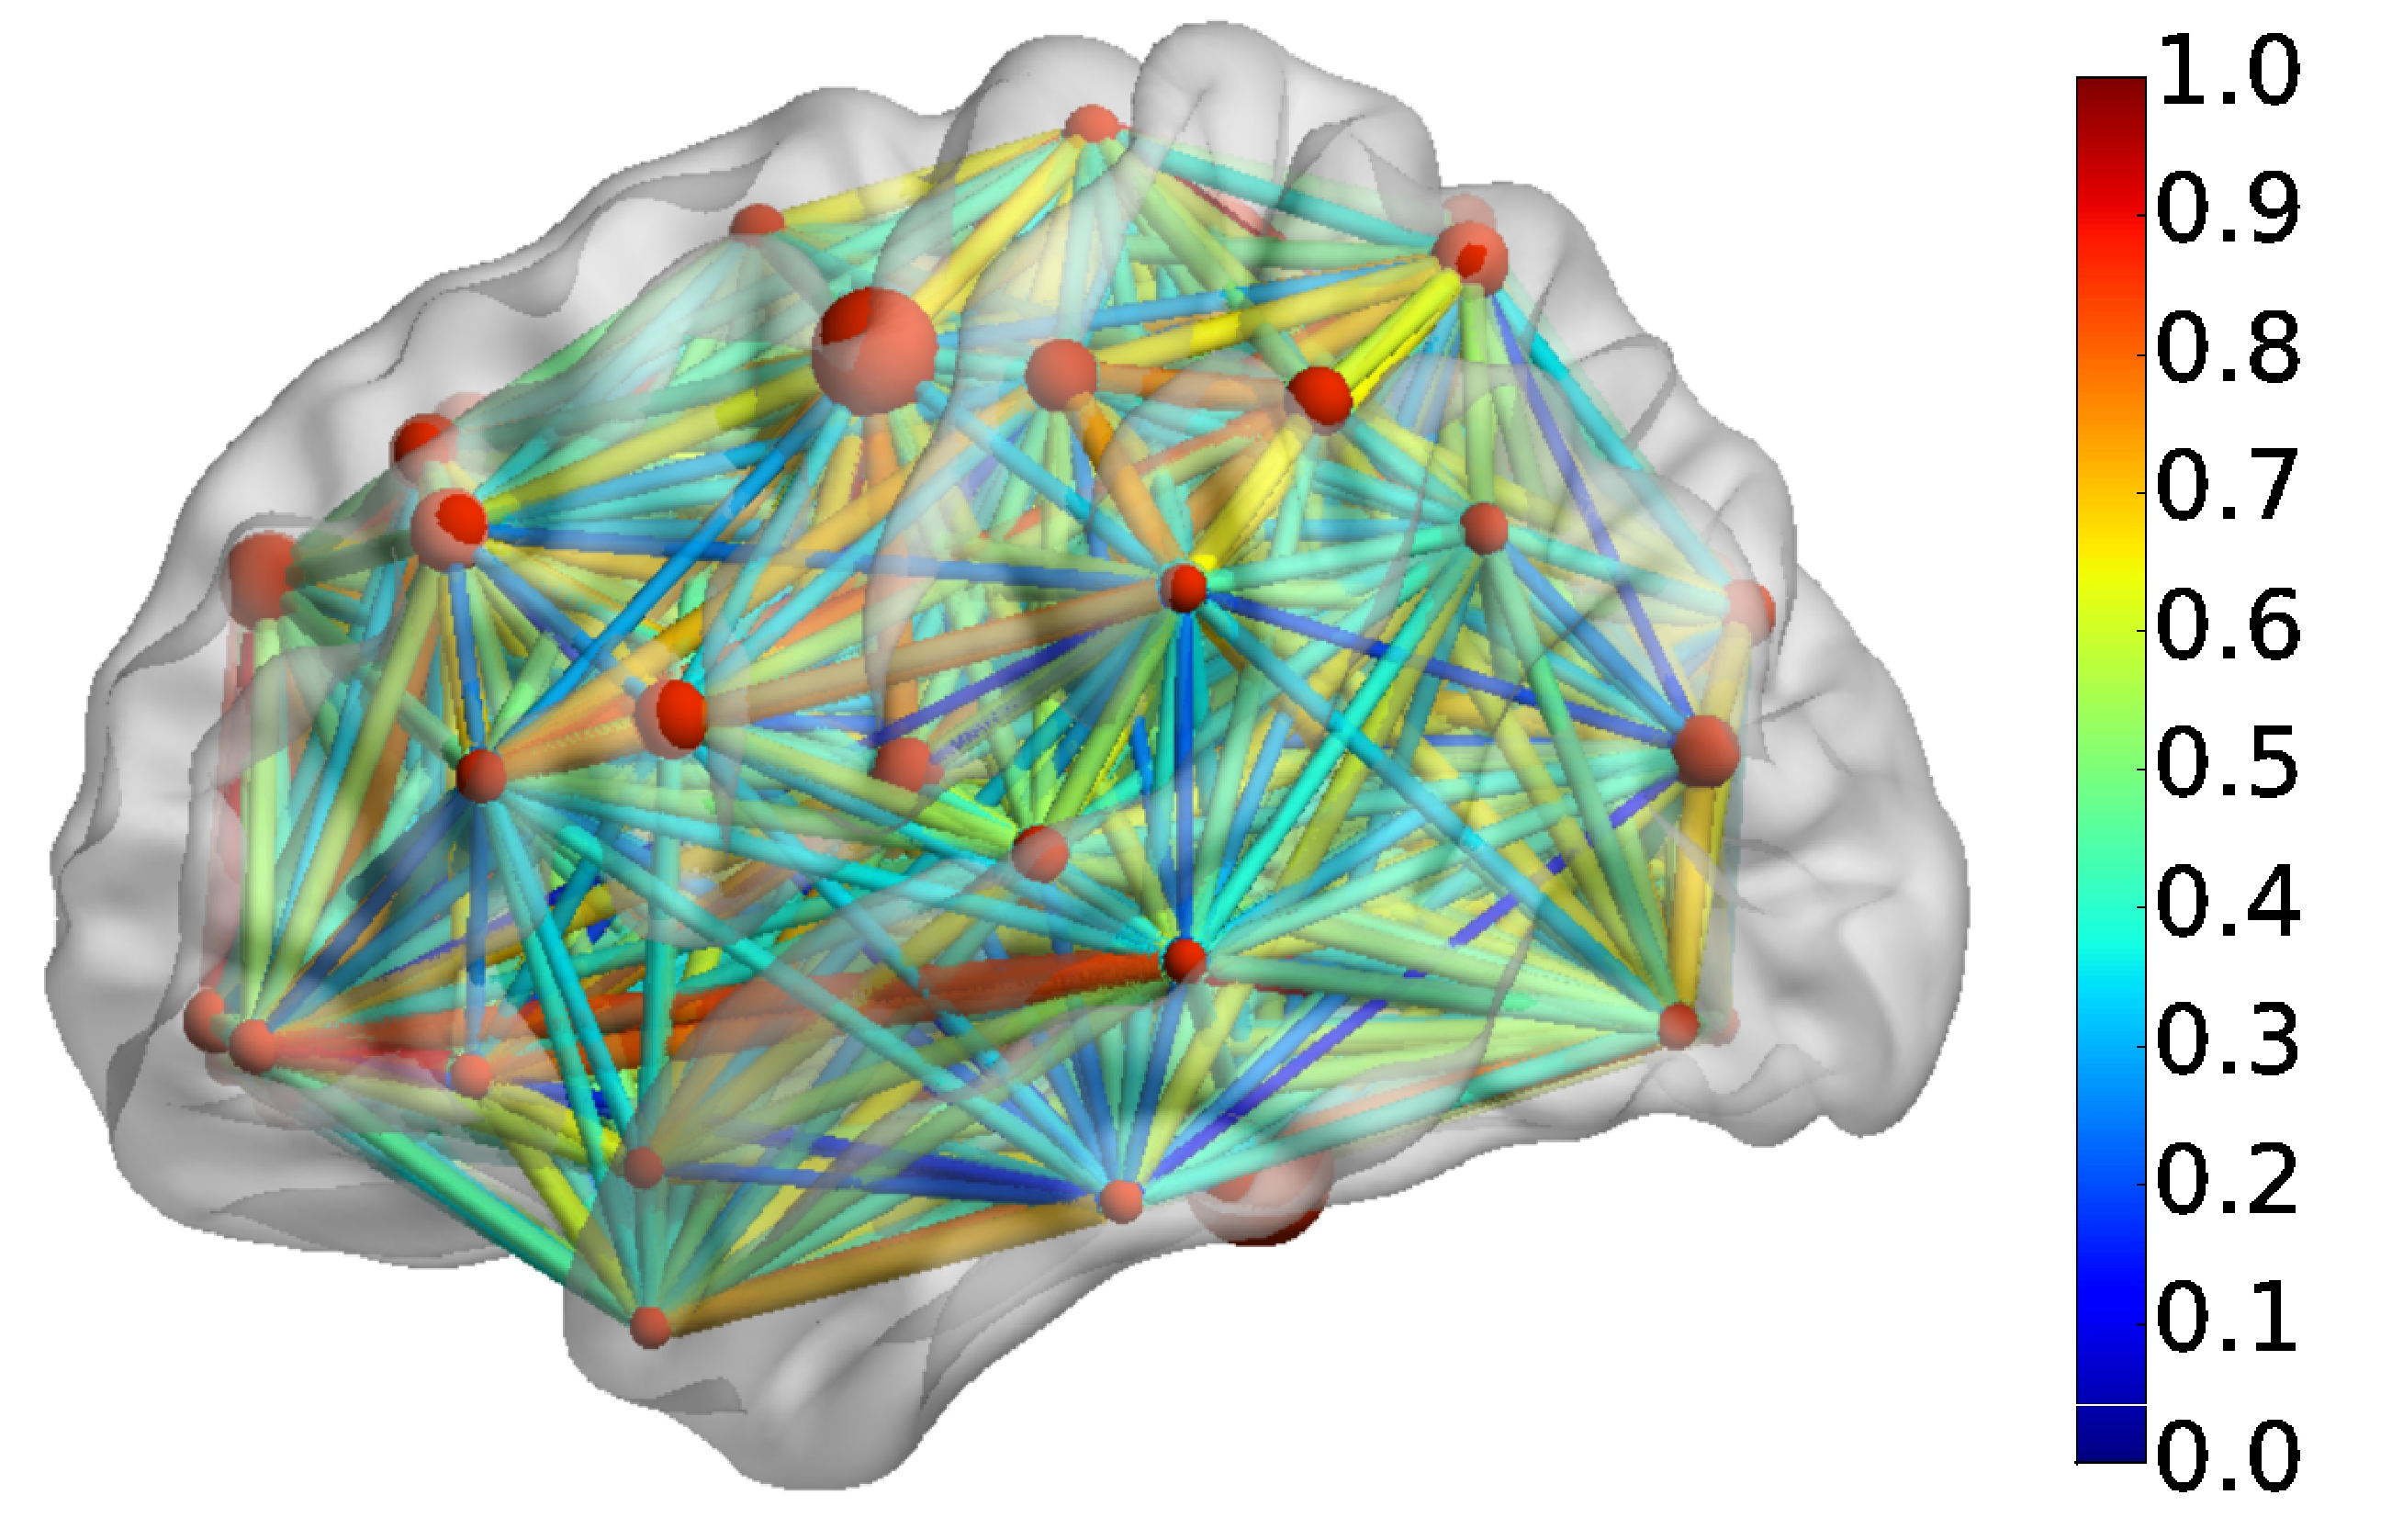
\includegraphics[width=0.49\textwidth]{Figures/FCM_brain.eps} 
	 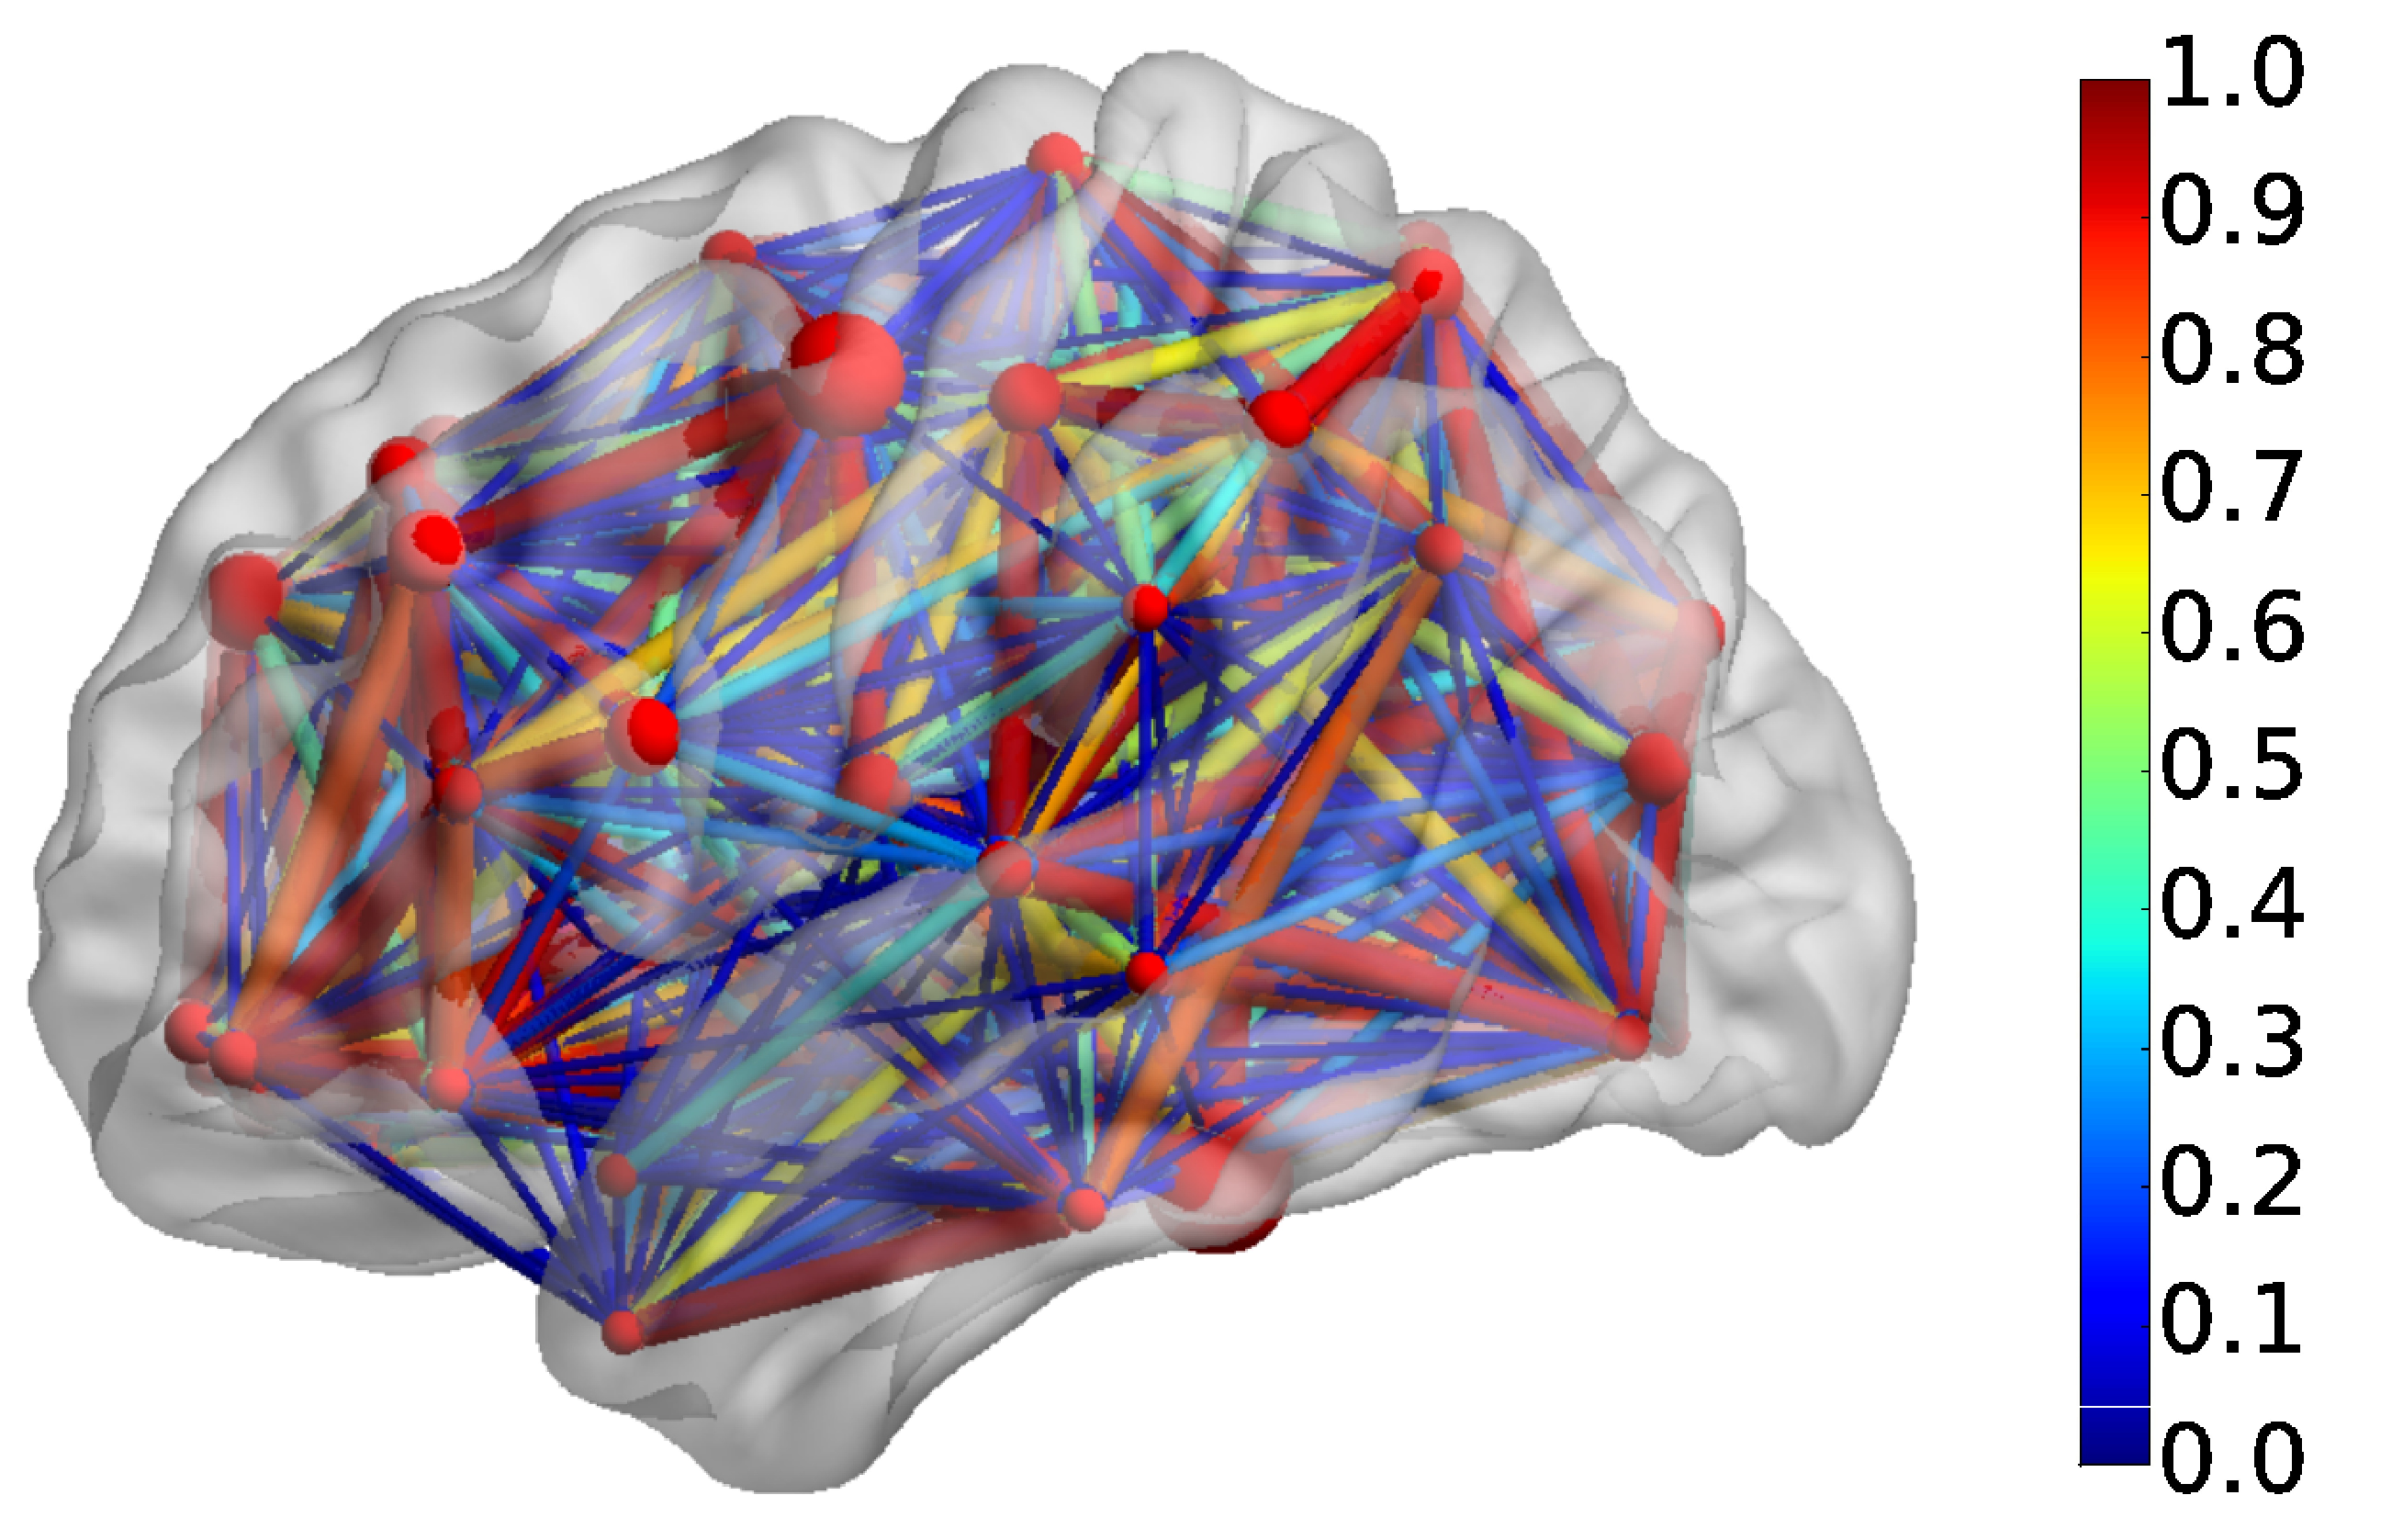
\includegraphics[width=0.49\textwidth]{Figures/ACM_brain.eps} 
    \rule{35em}{0.5pt}
  \caption[Empirical FCM and ACM in cortex]{3D sagittal visualization of FCM and ACM on the human cortex with the \textsc{BrainNet Viewer} \citep{XYZ13}. } 
  \label{fig:Empirical FCM and ACM in cortex}
 	
\end{figure} 

Figure 2.1 represents empirically captured FCM and ACM. All correlation coefficients in FCM appear in the range [0,1] as well as all probability values in ACM. Both matrices are symmetric. A correlation value close to 1 in FCM indicates that the quantified functional activities of corresponding nodes highly resemble each other. A probability value close to 1 in ACM demonstrates that corresponding nodes are most likely connected by fiber tracks in white matter. Although some node pairs are not anatomically coupled at all in ACM (cold colors), they could be functionally coupled in FCM (hot colors).    

FCM and ACM are embedded in human cortex in Figure 2.2 \citep{XYZ13}. All nodes are presented with equal size and black color independent of their topological properties. However, edges have different thickness and color distribution according to correlation coefficients and probability values with respect to FCM and ACM. 
 
   
\section{The Brain Graph}

The brain graphs considered here are derived from two sets of empirical brain connectivity maps: FCM and ACM obtained from fMRI-BOLD and DW-MRI techniques, respectively. Those data sets represent measurements from $N=90$ cortical and sub-cortical regions labeled with AAL, represented by nodes in the graph. The nodes can be connected to each other by means of "edges". If the graph is constructed on the FCM, edges are interpreted as correlation strengths between the functional BOLD activity of two nodes. If the graph is built on the ACM, an existing edge is considered as the probability of two nodes to be structurally connected by fiber tracks in white matter.

The brain graphs in this project are generated through binarizing the functional connectivity matrix (FCM) and anatomical connectivity matrix (ACM). Binarization here means converting all the values in a given matrix into 1's and 0's via thresholding. Because of the nature of their definition, both empirical data sets have values between 0 and 1, reflecting a correlation strength in case of FCM or a probability value in case of ACM. We arbitrarily define a threshold value $r$ for the strength of correlations in FCM. Then, the values greater and equal to $r$ are assigned the value 1, while others are set to 0. This thresholding is applied by means of the strength of probability value, $p$, for the ACM. The binarized matrix is the basis of brain graph construction, and it is commonly known as \textit{adjacency matrix}. The \textsc{Networkx} software package in \textsc{PYTHON} is used to built graphs given adjacency matrices. Neither the direction of functional or anatomical connectivity between nodes, nor any other values apart from 0 and 1  are encoded in the adjacency matrices,  so that the resulting graphs are considered as "undirected" and "unweighted". In other words, all existing edges are thought to be of uniform weight and nodes interact both ways along an edge connecting them. 

\begin{figure}[htbp]
 %\begin{tabular}{cc}
  \centering
	 \includegraphics[width=0.45\textwidth]{Figures/FCM.eps} 
	 \includegraphics[width=0.45\textwidth]{Figures/Sample_Adj.eps} 
	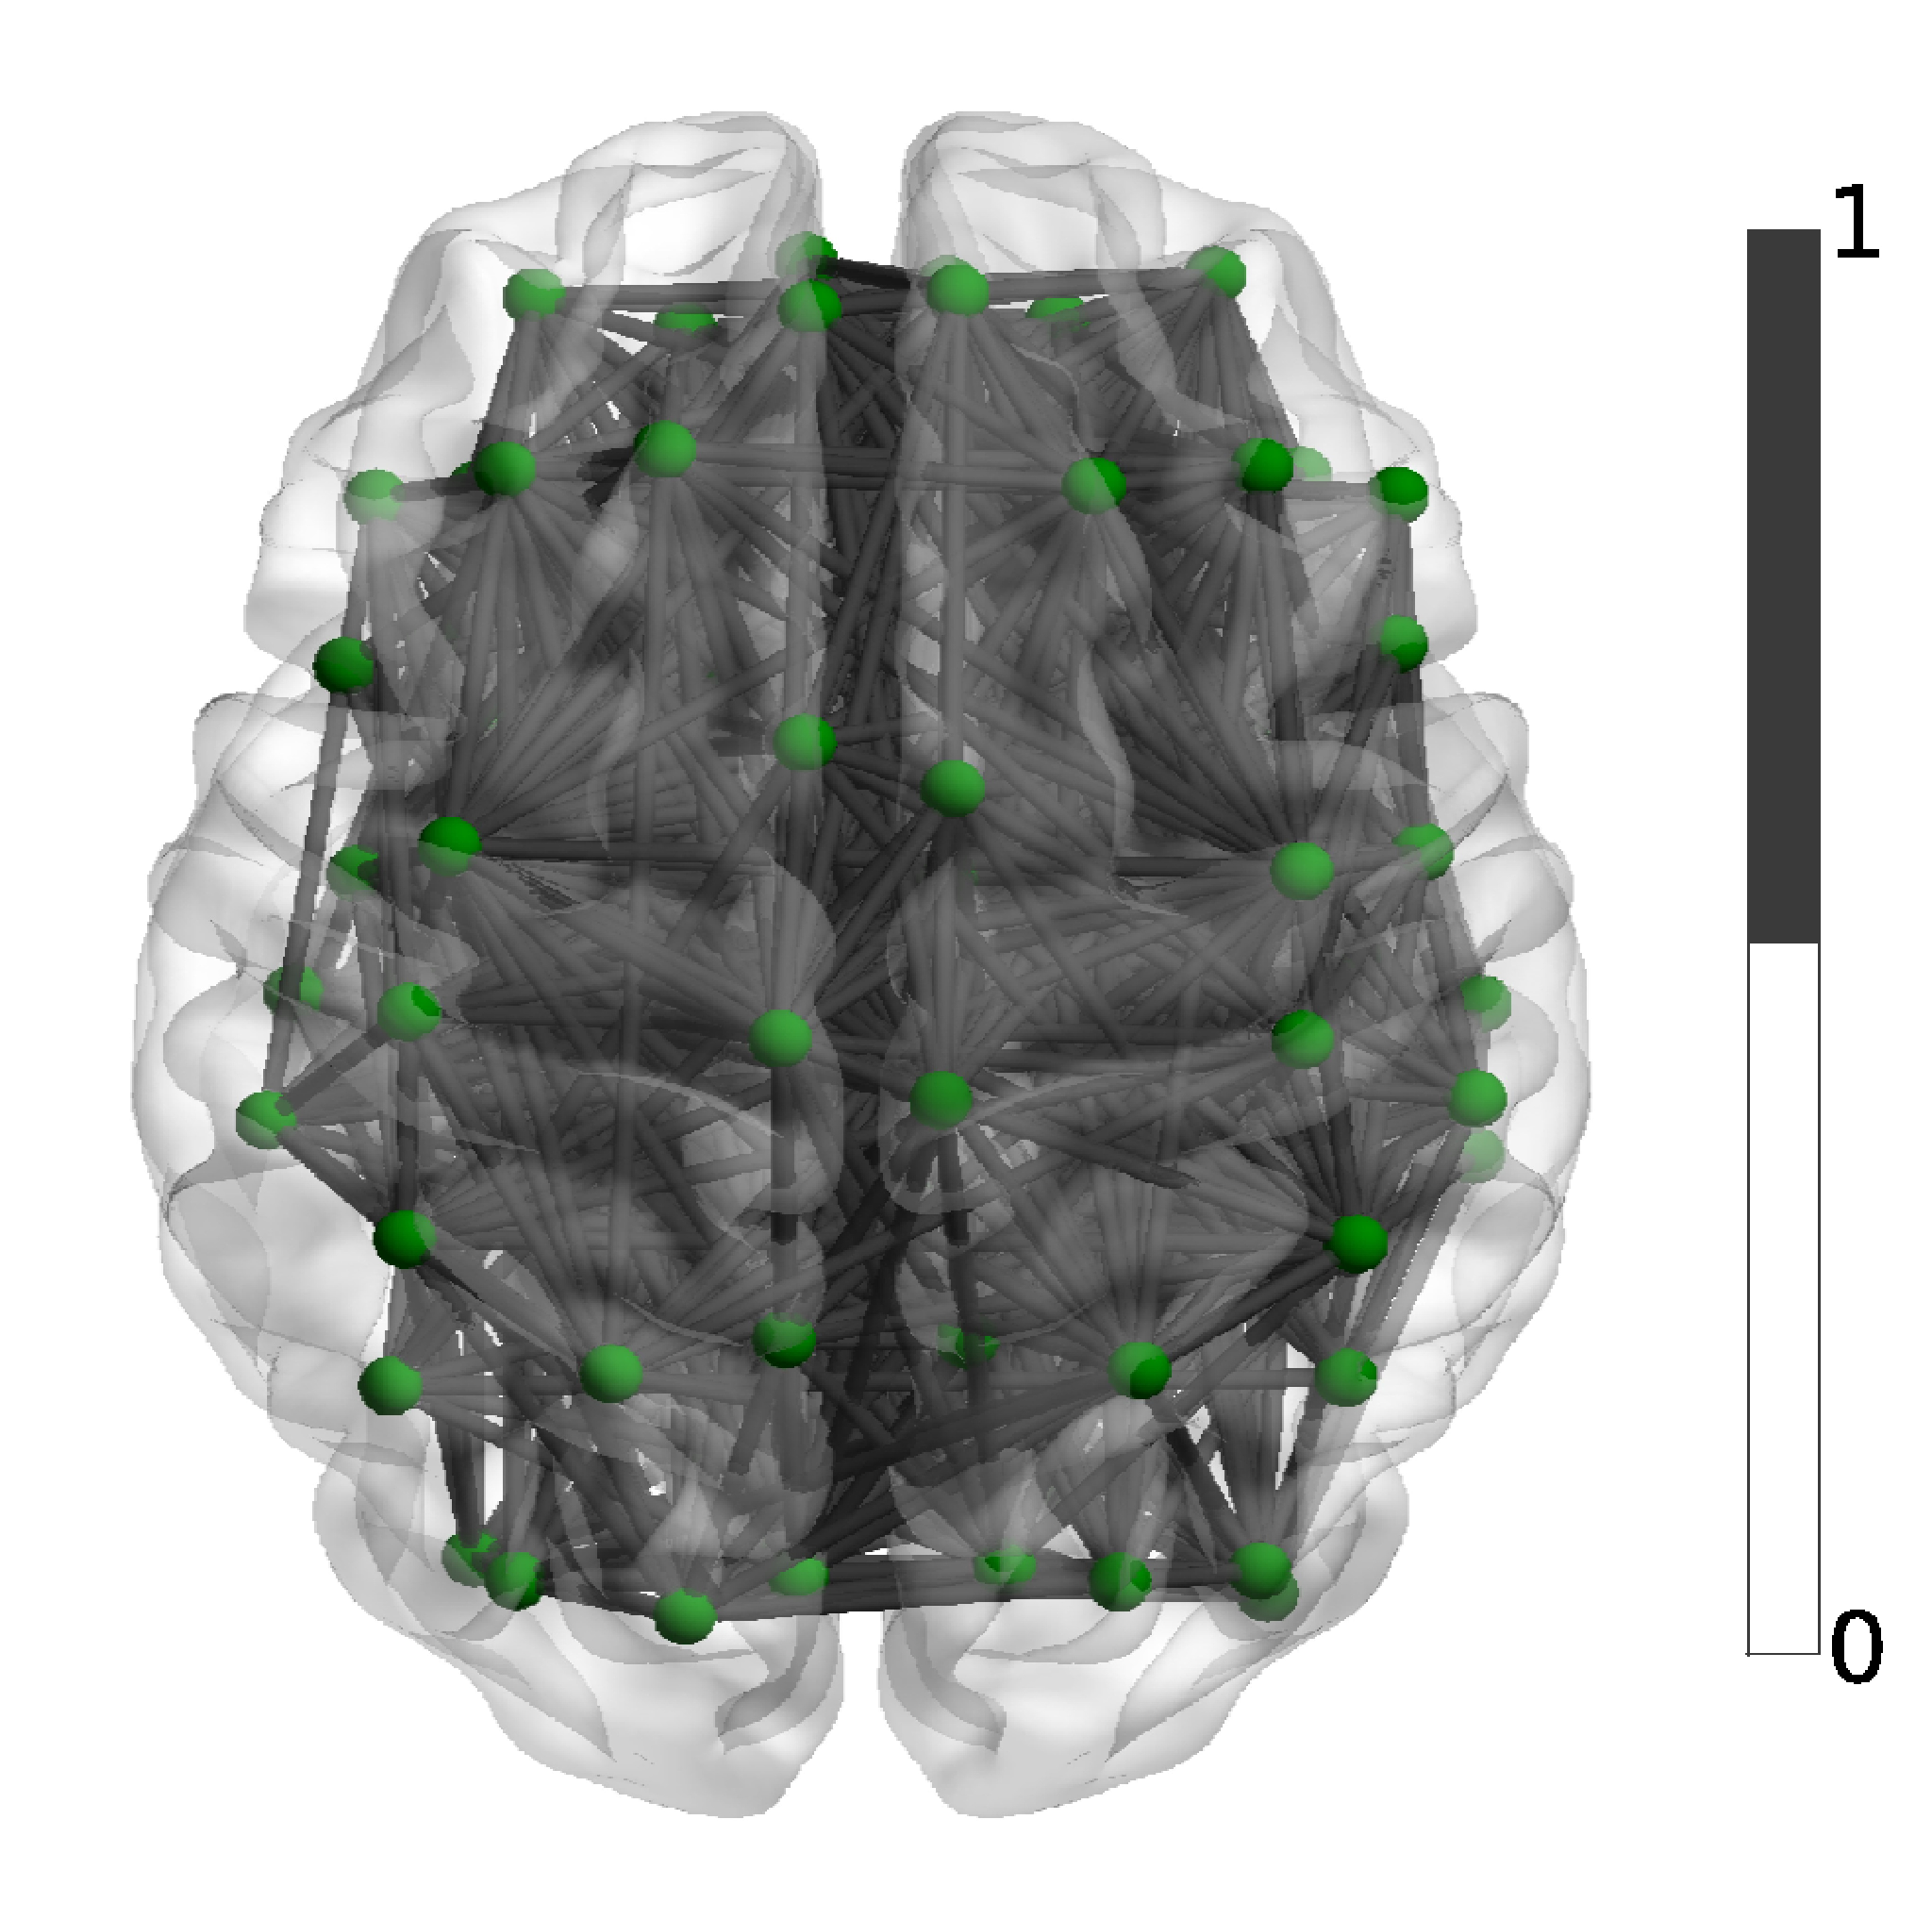
\includegraphics[width=0.45\textwidth]{Figures/Sample_Adj_brain.eps}  
   \includegraphics[width=0.45\textwidth]{Figures/brain_graph.png}      

    \rule{35em}{0.5pt}
  \caption[Binarizing via thresholding]{How to build a brain graph : The empirical data matrix derived from fMRI-BOLD technique (on the upper left) is binarized via a threshold value $r=0.55$ and its corresponding adjacency matrix (on the upper right). The black spots represent 1's indicating edges between nodes, whereas the white squares represent 0's implying no edge at all. The adjacency matrix is embedded on human cortex axially (on the lower left) with \textsc{BrainNet Viewer} \citep{XYZ13} and the brain graph derived from the adjacency matrix with \textsc{NETWORKX} (on the lower right).}
  \label{fig:Binarizing via thresholding}
 %\end{tabular}	
\end{figure}

Figure 2.1 illustrates the exemplary construction of a brain graph from the FCM. All correlation values among the cortical and sub-cortical regions in the empirical fMRI-BOLD data lie between 0 and 1. 3D axial cortex visualization represents only the existing edges with black edges among the nodes. The adjacency matrix (AM) is filled out only with 1's and 0's indicating functionally connected and unconnected nodes, whose correlated BOLD activity is equal to or greater than $r=0.55$. The algorithm \textsc{Networkx} builds the corresponding graph of an adjacency matrix. The AM obtained from an ACM would look similar, but would represent the probability of two nodes to be anatomically connected above a predefined threshold $p$. 

The following sections will cover randomization methods reshuffling the brain graphs and introduce some of the topological concepts characterizing brain graphs as well as random networks.



\section{Randomization Methods}





\subsection{Erd\H{o}s-R\'{e}nyi Type Randomization}

Given a total number of nodes $N$, Paul Erd\H{o}s and Alfr\'{e}d R\'{e}nyi produced an undirected graph $G(N,P)$, in which the presence of any edge between two nodes is assigned a probability $P$. 
The average total number of edges $L$ in an  Erd\H{o}s-R\'{e}nyi type random graph is $\binom {N} {2}P$, with a binomial distribution for the number of edges per node.

New randomization techniques arise through modifying the Erd\H{o}s-R\'{e}nyi method, e.g. given $N$ and $L$, a graph $G(N,L)$ can be picked uniformly random out of set of all potential graphs having $N$ nodes and $L$ edges. The probability for a graph to be picked among all the others is $\frac{L}{\binom {N}{2}}  $. One can study the various aspects of $G(N,P)$ and $G(N,L)$ even more detailed, but for the sake of simplicity, Erd\H{o}s-R\'{e}nyi model will not discussed further here.

\begin{figure}[htbp]
 %\begin{tabular}{cc}
  \centering
	\includegraphics[width=0.30\textwidth, height=40mm]{Figures/f1.png}  
	\includegraphics[width=0.30\textwidth, height=40mm]{Figures/f2.png} 
    \includegraphics[width=0.30\textwidth, height=40mm]{Figures/f3.png}

    \rule{35em}{0.5pt}
  \caption[Erdos-Renyi Example]{An illustration of the set of all $G(N,L)$ type random graphs with $N=3$ and $L=2$.}
  \label{fig:Erdos-Renyi Example}
 %\end{tabular}	
\end{figure}

Figure 2.2 illustrates all possible graphs having 3 nodes and 2 edges. One of those 3 simple graph is chosen uniformly random for the $G(N,L)$ randomization type, so that each graph is chosen with probability $P=\dfrac{1}{3}$.  

The $G(N,L)$ type randomization is the first method used to derive random graphs from the adjacency matrices of FCM and ACM in this project. Both matrices have $N=90$ nodes, however $L$ changes for each brain graph according to the applied threshold level and therefore is always recalculated. 

\subsection{Double-Edge-Swap Type Randomization}

The \textit{degree} $k_i$ of a node $i$ is defined as the number of edges connected to that node. The double-edge-swap method manipulates a given graph by swapping two existing edges among four nodes, while keeping the node degrees fixed. 


\begin{figure}[htbp]
 %\begin{tabular}{cc}
  \centering
	\includegraphics[width=0.32\textwidth, height=50mm]{Figures/G1_swap.eps}  
    \includegraphics[width=0.32\textwidth, height=50mm]{Figures/G2_swap.eps}  
	\includegraphics[width=0.32\textwidth, height=50mm]{Figures/G3_swap.eps} 
    \rule{35em}{0.5pt}
  \caption[Double-Edge-Swap Example]{Swapping edges between 2 paired nodes}
  \label{fig:Double-Edge-Swap Example}
 %\end{tabular}	
\end{figure}

Figure 2.3 illustrates randomly chosen double edges in a sample graph to be swapped. After the existing edges are removed, the new pair of nodes are rewired. The degree of each node is the same before and after swapping; degrees of nodes $k_1 = 1$, $k_2=1$, $k_3=1$, $k_4=1$ are all fixed in each graph. Although the randomly constructed graphs with the double-edge-swap method are expected to have same degrees, the latter is not a unique property identifying a graph.

The \textit{degree distribution} is the probability distribution of node degrees over the whole graph. Conservation of each $k_i$ preserves the degree distribution, however, preserving degree distribution does not guarantee to fix $k_i$ values. We will discover in the next section how to preserve degree distribution by altering node degrees.

\subsection{Preserved-Degree-Distribution Type Randomization}

The preserved-degree-distribution method randomizes a given network by adding, removing or rewiring its edges randomly while recovering its degree distribution $P(k)$. The idea is to reassign edge indices in the graph, meaning that the degree of individual nodes may change. P(k) is defined with the following equation,

\begin{equation}
P(k) = \sum_{k' \geq k} p(k')
\end{equation}

where $p(k')$ is the probability of a node to have degree number $k'$ \citep{BAR99a}.


\begin{figure}[htbp]
 %\begin{tabular}{cc}
  \centering
	\includegraphics[width=0.45\textwidth, height=60mm]{Figures/G_degree_dist_1.eps}  
	\includegraphics[width=0.45\textwidth, height=60mm]{Figures/G_degree_dist_2.eps}    
    \rule{35em}{0.5pt}
  \caption[Degree Distribution 2D Example]{Reconstruction of a given graph (on the left) with degree-distribution-preservation model (on the right). $k_i=\{3,1,1,1\}$ in the original graph and $k_{i}=\{1,0,1,3,1\}$ in the randomized graph. }
  \label{fig:Degree Distribution Example}
 %\end{tabular}	
\end{figure}

The algorithm is thought to add-remove new nodes to a given graph while preserving $P(k)$ as shown in Figure 2.6. However, we randomize our brain graph with a conserved total number of nodes $N$ as well as $P(k)$. The figure is given only for a better visualization in order to distinguish preserved-degree-distribution randomization method and configuration model randomization, which will be introduced in the next section.

\begin{figure}[htbp]
 %\begin{tabular}{cc}
  \centering
	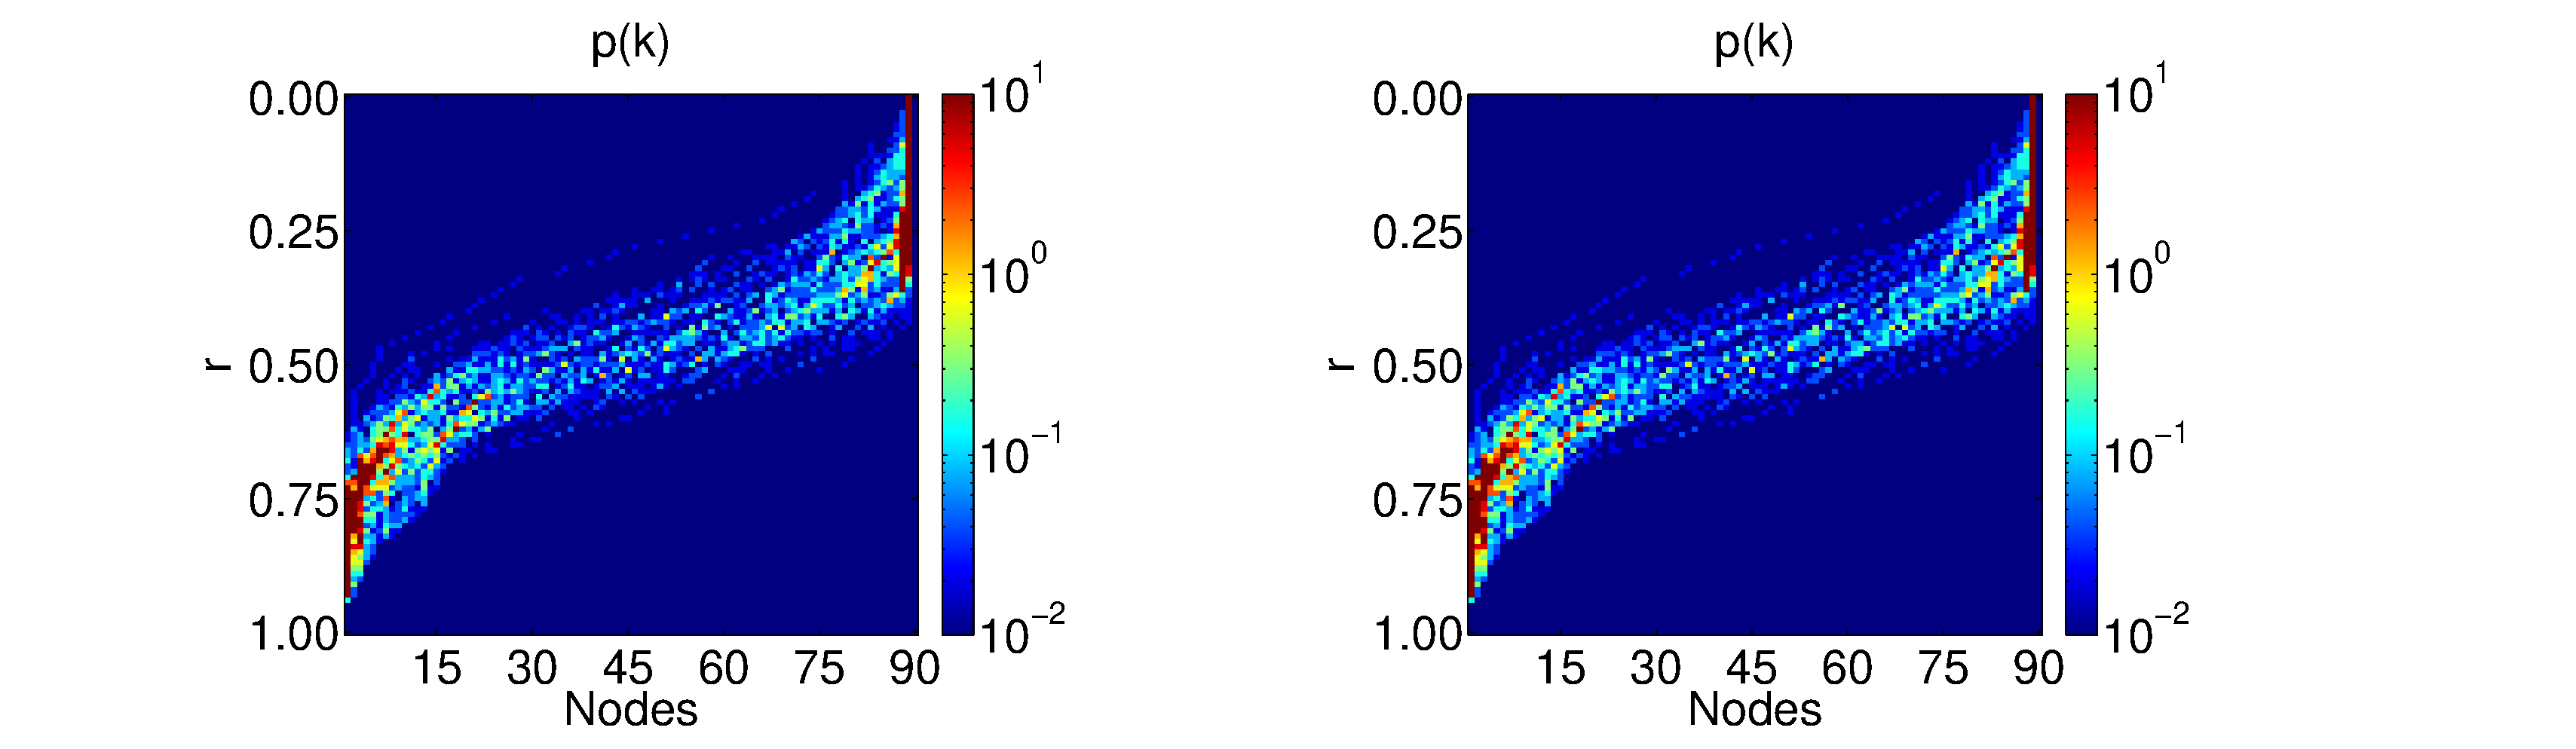
\includegraphics[width=\textwidth]{Figures/G_degree_dist.eps}  
    \rule{35em}{0.5pt}
  \caption[Degree Distribution 3D Example]{Heat maps for degree distributions of the brain graph obtained from FCM (on the left), and of the randomized graph with preserved-degree-distribution tool (on the right). Colorbars are in logarithmic scale with lower and upper limits : $[\log_{10} {10}^0 , \,  \log_{10} {10}^1]$}
  \label{fig:Degree Distribution 3D Example}
 %\end{tabular}	
\end{figure}

$P(k)$ is a global topological measure for a network, it can be illustrated over all nodes in the whole graph as in Figure 2.7. Node indexes are labeled on $x$ axis on heat maps, threshold $r$ values for adjacency matrices are given on $y$ axis. The preserved-degree-distribution method generates successfully a random graph with the same $P(k)$ as in the brain graph. 


\subsection{Configuration Model Randomization}

The \textit{degree sequence} of a graph is either its ascending or descending sequence of node degrees. The configuration model generates a random graph with a given degree sequence. The direct implementation of this model is to assign edges to the nodes randomly until the desired degree sequence is matched. The resultant random graph is expected to be a node-index-shuffled version of the original graph. However, these algorithms are non-trivial due to the occurrence of self-loops (node is connected to itself) and parallel edges (multiple edges connecting two nodes), which are both undesirable graph properties in this project. 

\begin{figure}[htbp]
 %\begin{tabular}{cc}
  \centering
	\includegraphics[width=0.45\textwidth, height=60mm]{Figures/G_config_1.eps}  
	\includegraphics[width=0.45\textwidth, height=60mm]{Figures/G_config_2.eps} 
    \rule{35em}{0.5pt}
    \caption[Degree Sequence Definition]{The degrees of the nodes in the original graph (on the left): $k_0 = 2$, $k_1 =1$, $k_2=2$, $k_3=3$ and that of the randomized graph (on the right) : $k_0 = 3$, $k_1 =2$, $k_2=1$, $k_3=2$. The degree sequence in non-increasing order in both graphs : $\{3,\,2,\,2,\,1\}$}
  \label{fig:Degree Sequence Definition}
 %\end{tabular}	
\end{figure}

Figure 2.8 points out the relevance of the degree sequence to the node degrees. Moreover, one should not confuse degree distribution and degree sequence.   

The configuration model variant used here is the expected-degree-graph method, which excludes self-loops and parallel edges. This algorithm receives the list of the expected degree sequence as an input $(k_u, k_v, k_m, k_l, ...)$, and assigns edges between nodes with a predefined probability $P_{uv}=\dfrac{k_u k_w}{\sum_{i}k_i}$. This method does not guarantee to construct graphs with exactly the same given degree sequence but with the closest possible sequence.  



 
\subsection{Partial Randomization}
 
The partial randomization method  reconstructs a graph (say A) with partial rewirings with respect to a second graph (say B) while keeping the degree distribution the same as in A. The analogy of this algorithm is to perform rewirings in the adjacency matrix of A, while avoiding any edge generation which already exist in the B. In other words, the choice of edges to be performed rewirings in A is limited with respect to the B. 

In this project, the functional connectivity (FC) adjacency matrix is partially rewired with respect to the anatomical connectivity (AC) adjacency matrix.  This means doing such rewirings among the nodes in FCM only if these nodes are not structurally connected in the brain with probability above a given value. The same procedure is done to randomize AC adjacency matrix partially with respect to FC adjacency matrix.  This time nodes in ACM can be linked only if they are not functionally correlated above a given threshold.   

\begin{figure}[htbp]
 %\begin{tabular}{cc}
  \centering
	\includegraphics[width=\textwidth, height=55mm]{Figures/p1.png}  
    \rule{35em}{0.5pt}
    \caption[Partial Randomization Example]{Graph A is performed a partial randomization with respect to graph B. While the partial randomization tool rewires edges in A, it avoids creating such edges that exist in B.}
  \label{fig:Partial Randomization Example}
 %\end{tabular}	
\end{figure}

Representative graphs $A$ and $B$ in Figure 2.9 can be thought as FCM and ACM, respectively. In this case, $A \,\, random$ is the partially randomized graph of FCM with respect to ACM.


The brain graph and randomly generated graphs will be identified in terms of their topological properties in the following sections. For simplicity the abbreviations are introduced in the table below. 

\begin{table}[h]
\begin{center}
\caption[Abbreviations]{Abbreviations for the brain graph and the randomly constructed graphs. }
\begin{tabular}{ l | c | r }
  Abbreviation & Description & method \\
  \hline  \hline                     
  R0 & the brain graph						  & \textsc{networkx} \\ \hline
  Ra & Erd\H{o}s-R\'{e}nyi, G(N,L)            & \textsc{networkx} \\ \hline
  Rd & double-edge-swap            			  & \textsc{networkx} \\ \hline
  Rh & preserved-degree-distribution		  & \textsc{BCT} 	 \\ \hline  
  Rg & configuration model       			  & \textsc{networkx} \\ \hline
  Rk & partial randomization            	  & \textsc{BCT} 	 \\ \hline  
  \hline  
\end{tabular}
\label{table:Abbreviations}
\end{center}
\end{table}	

\section{Network Characterizations}

\subsection{Network Density}
The \textit{average degree} $\langle k \rangle$ of a network is proportional to the ratio of total number of edges $L$ to total number of nodes $N$ in a graph, 

\begin{equation}
\langle k \rangle = \frac{2L}{N}.
\end{equation}

It should be noted that in order to not count each edge twice, the total number of edges is divided by $N/2$ instead of $N$. The \textit{density} $\kappa$ of a network is a scaled version of average degree measurement. It is formulated as the ratio between $L$ and maximum number of possible edges $\binom{N}{2}$,

\begin{equation}
\kappa = \frac{2L}{N(N-1)}.
\end{equation}	

The measure of network density can be referred to as the total \textit{wiring cost} of the network \citep{RUB10}. The degree, average degree and network density are key scalar measures to characterize the topology of a network. There is for instance clinical evidence that reductions in nodal degree are associated with greater severity of local amyloid deposition in patients with Alzheimer's disease \citep{XYZ2009}. 

\begin{figure}[htbp]
 %\begin{tabular}{cc}
  \centering
	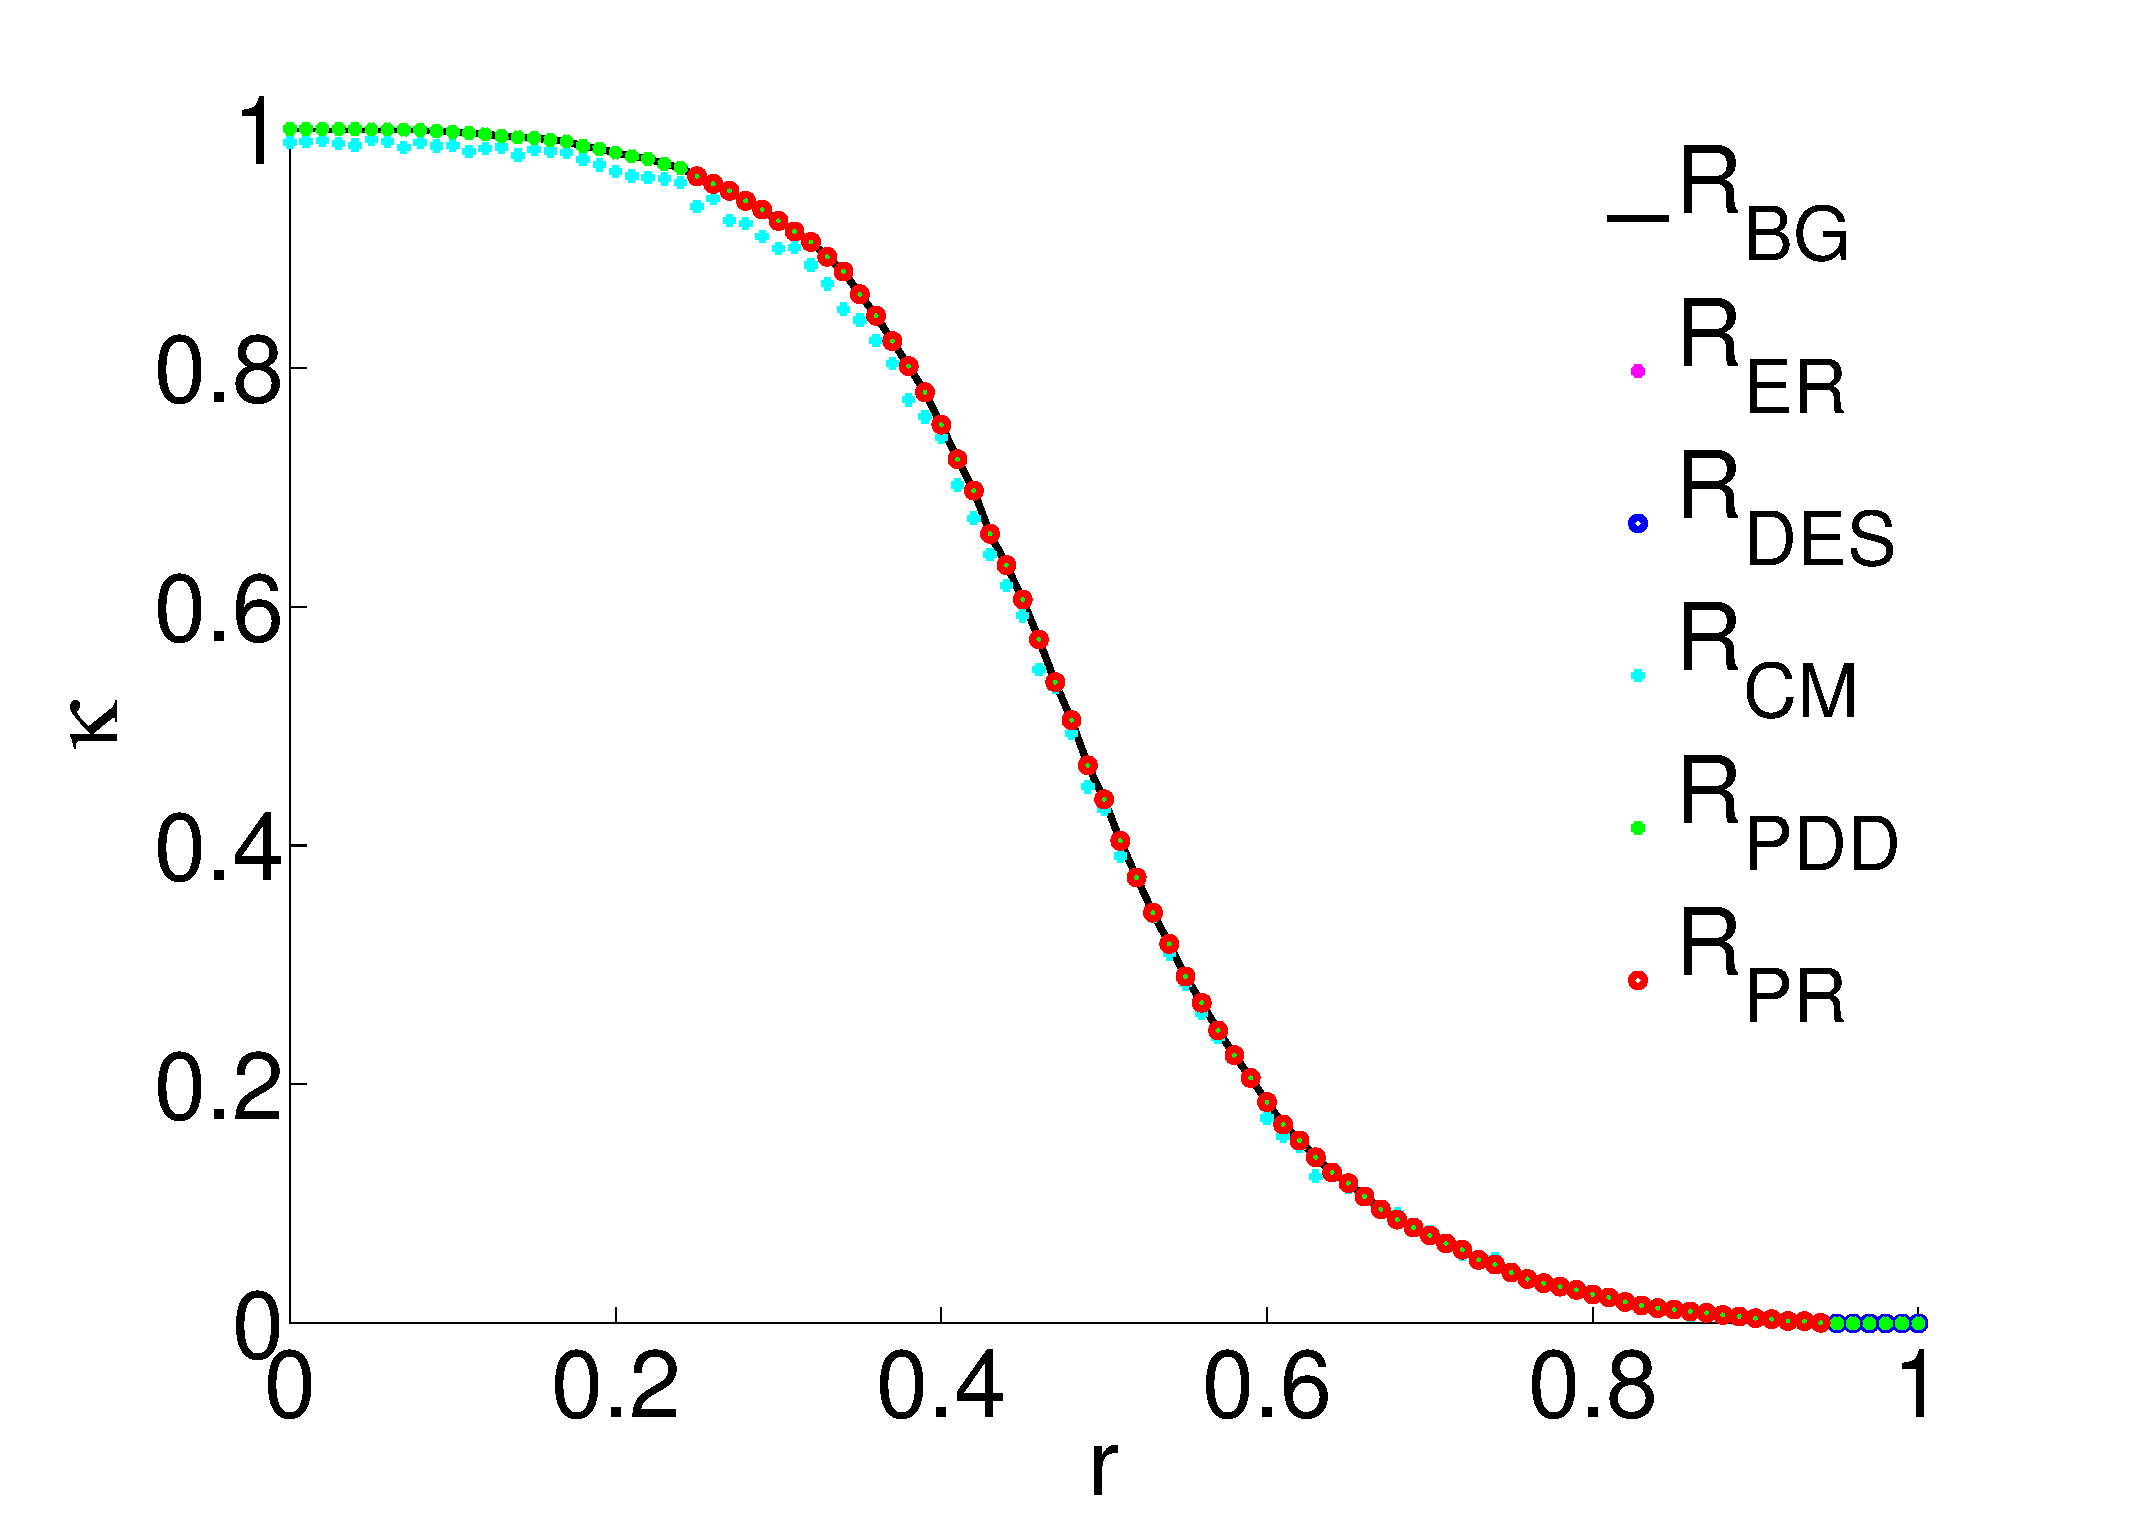
\includegraphics[width=0.48\textwidth, height=55mm]{Figures/Network_Density_Fnc.eps}
	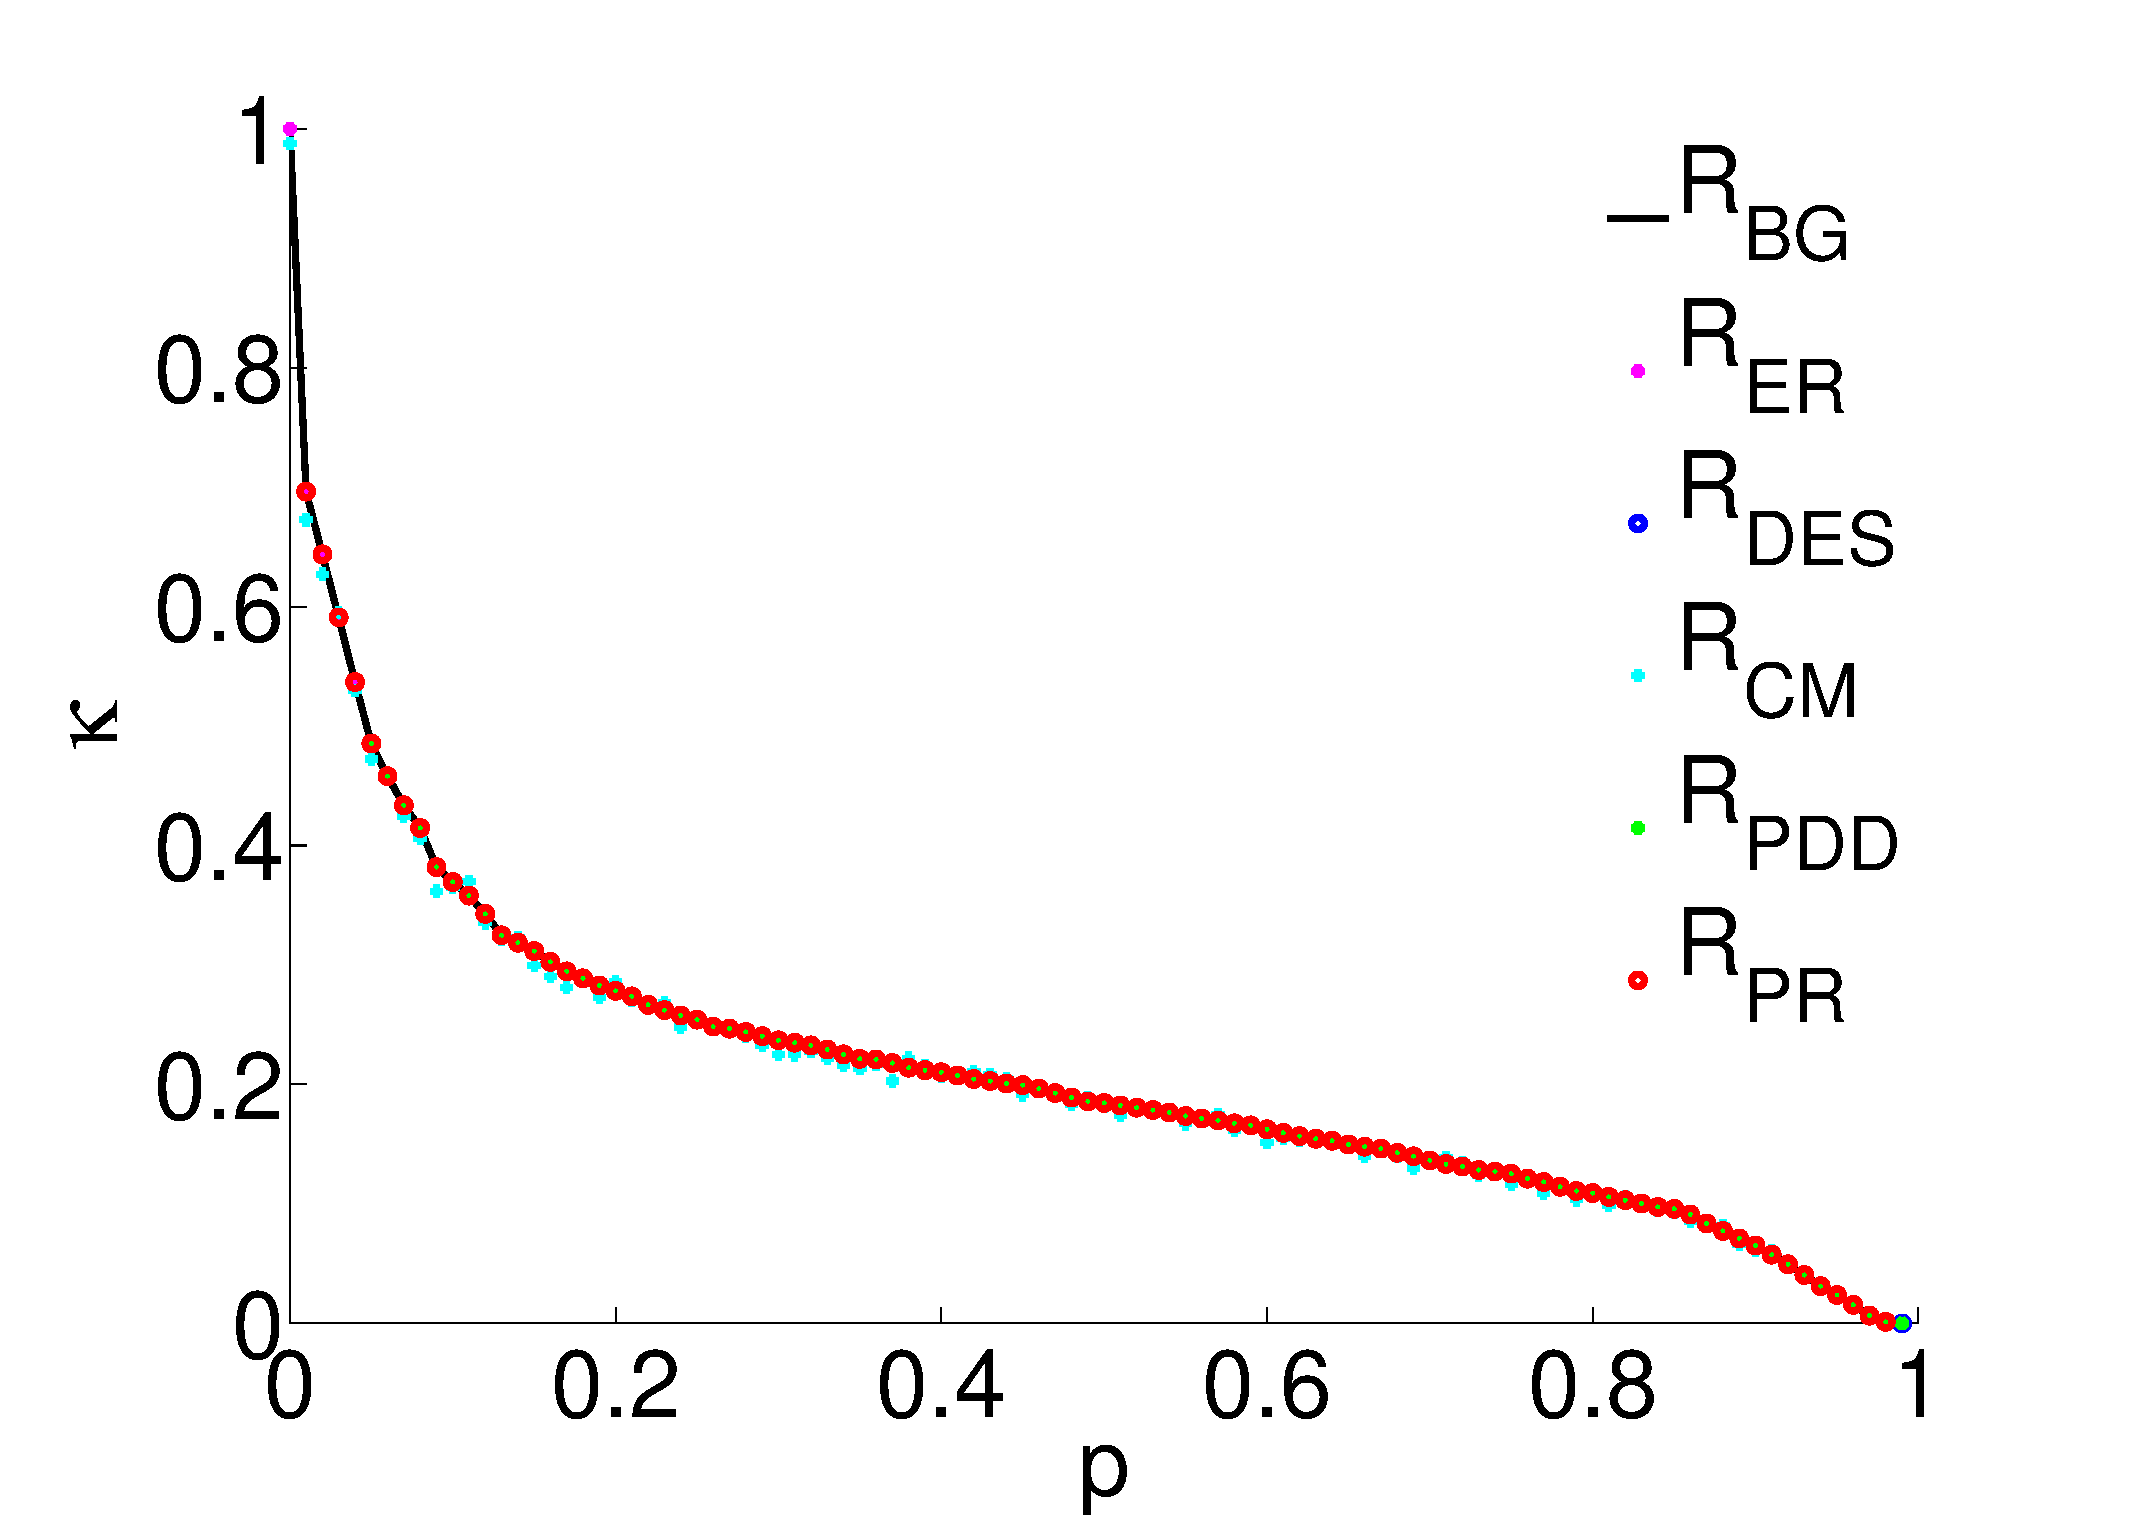
\includegraphics[width=0.48\textwidth, height=55mm]{Figures/Network_Density_Stru.eps}  
    \rule{35em}{0.5pt}
    \caption[Network Density]{Network density of the brain graphs and random graphs of FCM (on the left) and ACM (on the right). The abbreviations are chosen as described in Table 1.}
  \label{fig:Network Density}
 %\end{tabular}	
\end{figure}


The network density $\kappa$ can be considered a probability for all graphs in corresponding threshold $r$ and $p$ ranges. The random networks are built in such ways that they have the same number of nodes and almost the same $\kappa$ as in the brain graphs. However, the $\kappa$ is not a unique metric identifying a network.

All networks for FCM and ACM are densely connected for low $r$ and $p$. For the brain graph and randomized graphs of FCM, $\kappa$ decreases sigmoidally with $r$. In comparison, $\kappa$ decreases slower with $p$ for ACM graphs. It should be noted that all graphs have almost the same $\kappa$ values. 

Functional networks are likely to be denser than anatomical networks, as they will typically contain numerous connections between anatomically unconnected regions \citep{DAM09}. 

\subsection{Average Clustering Coefficient}
    
The \textit{average clustering coefficient} $C$ of a network is calculated through individual clustering coefficients $C_i$ of single nodes,

\begin{equation}
C = \frac{1}{n} \sum\limits_{i\epsilon N}C_i = \frac{1}{n}\sum\limits_{i\epsilon N} \frac{2t_i}{k_i(k_i -1)} .
\end{equation} 

where $t_i$ is the number of triangles around node $i$ and $k_i$ is the degree of node $i$ \citep{WAT98}. The clustering coefficient is a measure of segregation, that is the ability for specialized processing to occur within densely interconnected groups of brain regions \citep{RUB10}. It reveals how the individual nodes in a graph cluster together; how many neighbors of a node are neighbors of each other. 

\begin{figure}[htbp]
 %\begin{tabular}{cc}
  \centering
	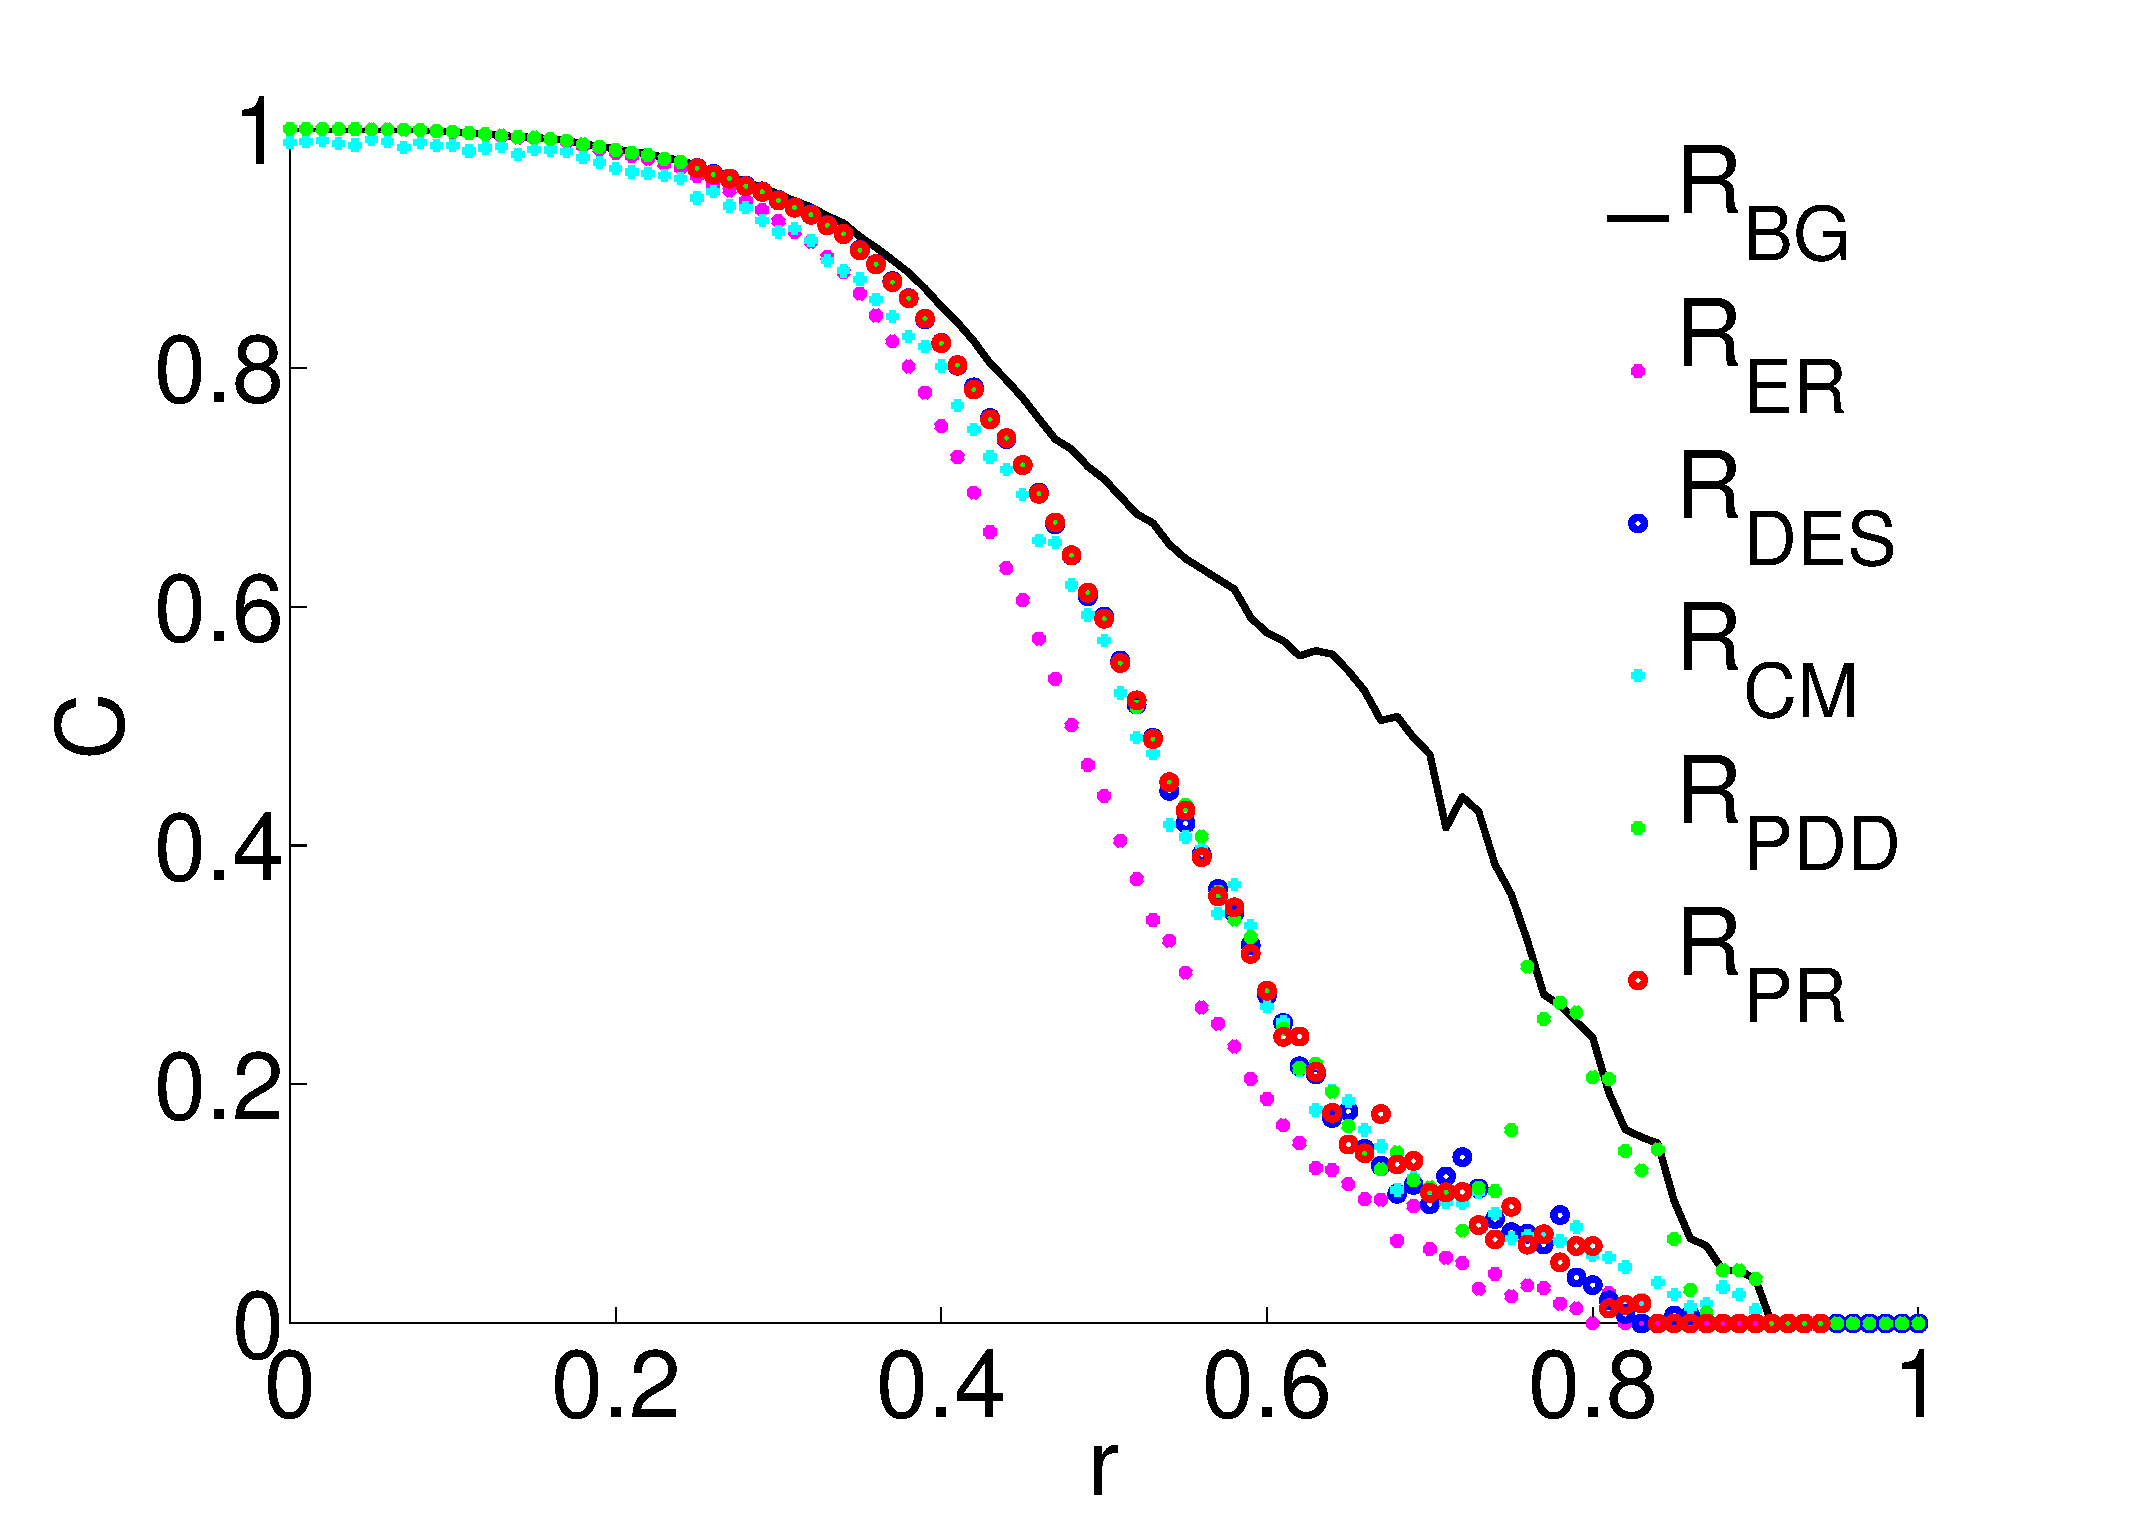
\includegraphics[width=0.48\textwidth, height=55mm]{Figures/Clustering_Coefficient_Fnc.eps}
	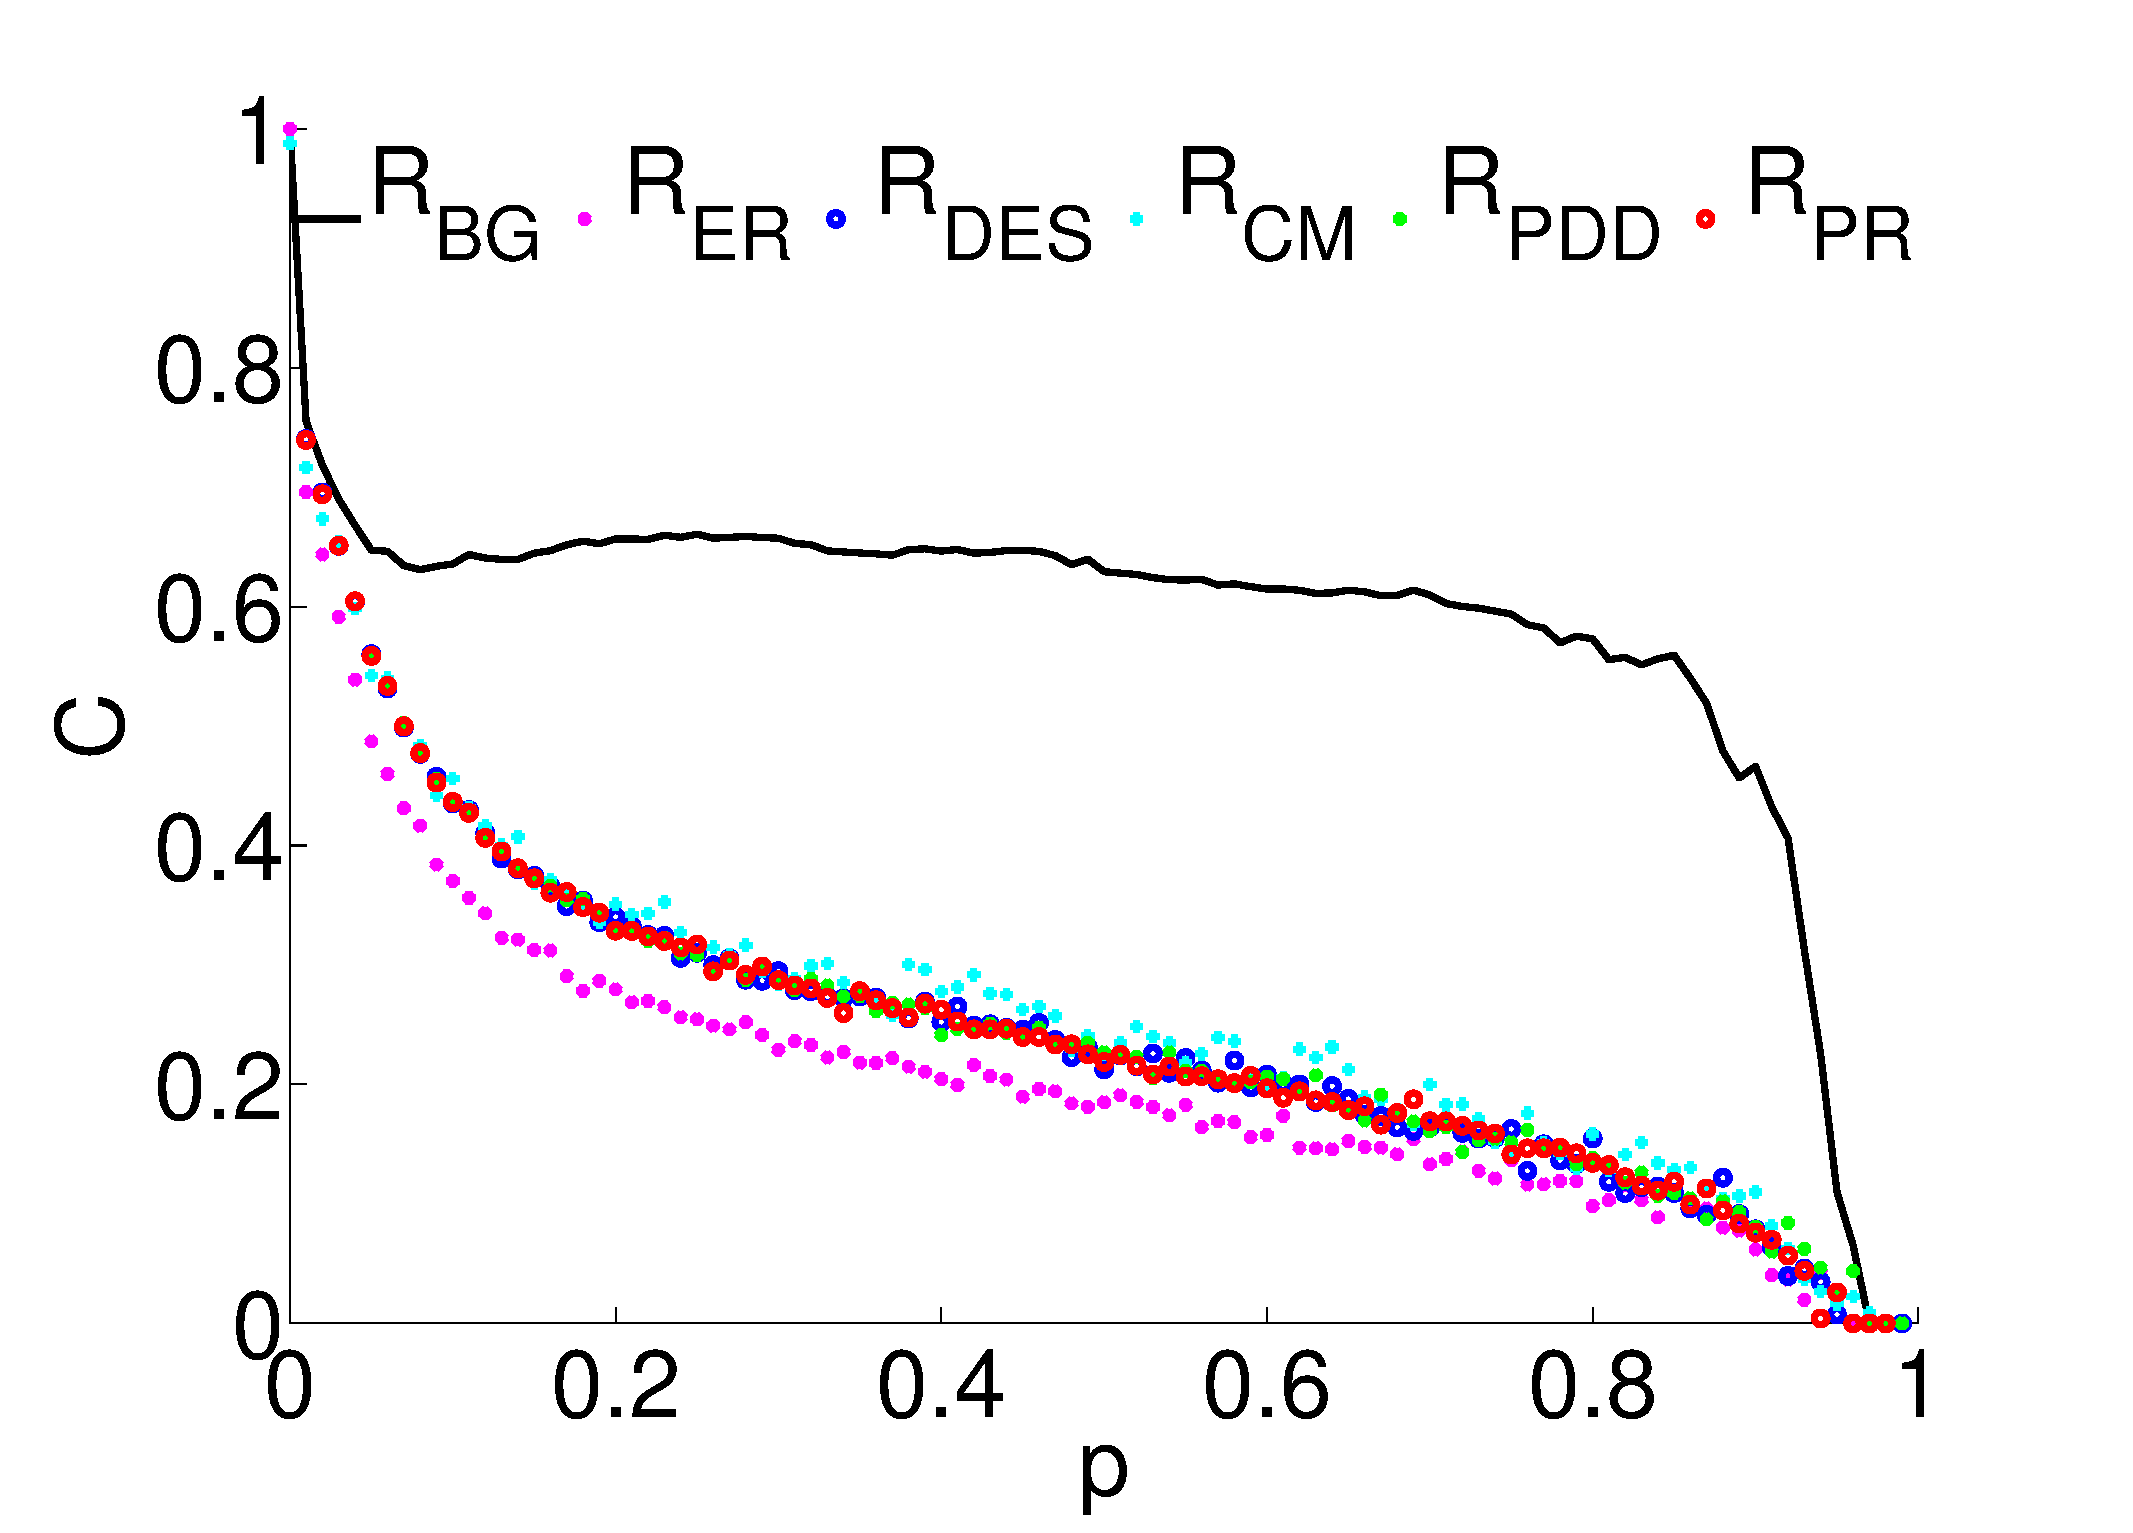
\includegraphics[width=0.48\textwidth, height=55mm]{Figures/Clustering_Coefficient_Stru.eps} 
    \rule{35em}{0.5pt}
    \caption[Clustering Coefficient]{Average clustering coefficient of the brain graphs and random graphs of FCM (on the left) and ACM (on the left). }
  \label{fig:Clustering Coefficient}
 %\end{tabular}	
\end{figure}

The clustering coefficient $C_i$ of a node $i$ is a measure of local connectivity and is highly correlated with the local efficiency of the information transfer \citep{LAT01}. The $C_i$ is formulated as the ratio of $t_i$ over all possible edges of the node $i$; $\binom{k_i}{2} $. The average clustering coefficient $C$ is a normalized version of $C_i$ for the whole network, yielding now a global property. All $C$ values are between 0 and 1. Figure 2.7 shows that at lower binarization thresholds, nodes tend to cluster more due to higher number of existing edges. The empirically obtained brain networks of FCM and ACM have the highest $C$ compared to random graphs. The local information transfer seems to be more efficient in the brain graphs.  The randomized graphs of ACM $Ra$, $Rd$, $Rh$ and $Rk$ share more nodes with lower degrees compared to $R0$.

\subsection{Transitivity}

Transitivity is a similar measure to the clustering coefficient, and also quantifies segregation in the network. It is defined as \citep{NEW03}
	
\begin{equation}
 T = \frac{\sum\limits_{i \epsilon N} 2 t_i}{\sum\limits_{i \epsilon N}k_i (k_i - 1)} .
\end{equation}	

If a node has links to two other nodes, transitivity inquires whether those two other nodes are also connected to each other. It asks, what percentage of triangles in the network is closed. Transitivity resembles clustering coefficient, however, it is defined only for the whole network rather than single nodes. 

\begin{figure}[htbp]
 %\begin{tabular}{cc}
  \centering
	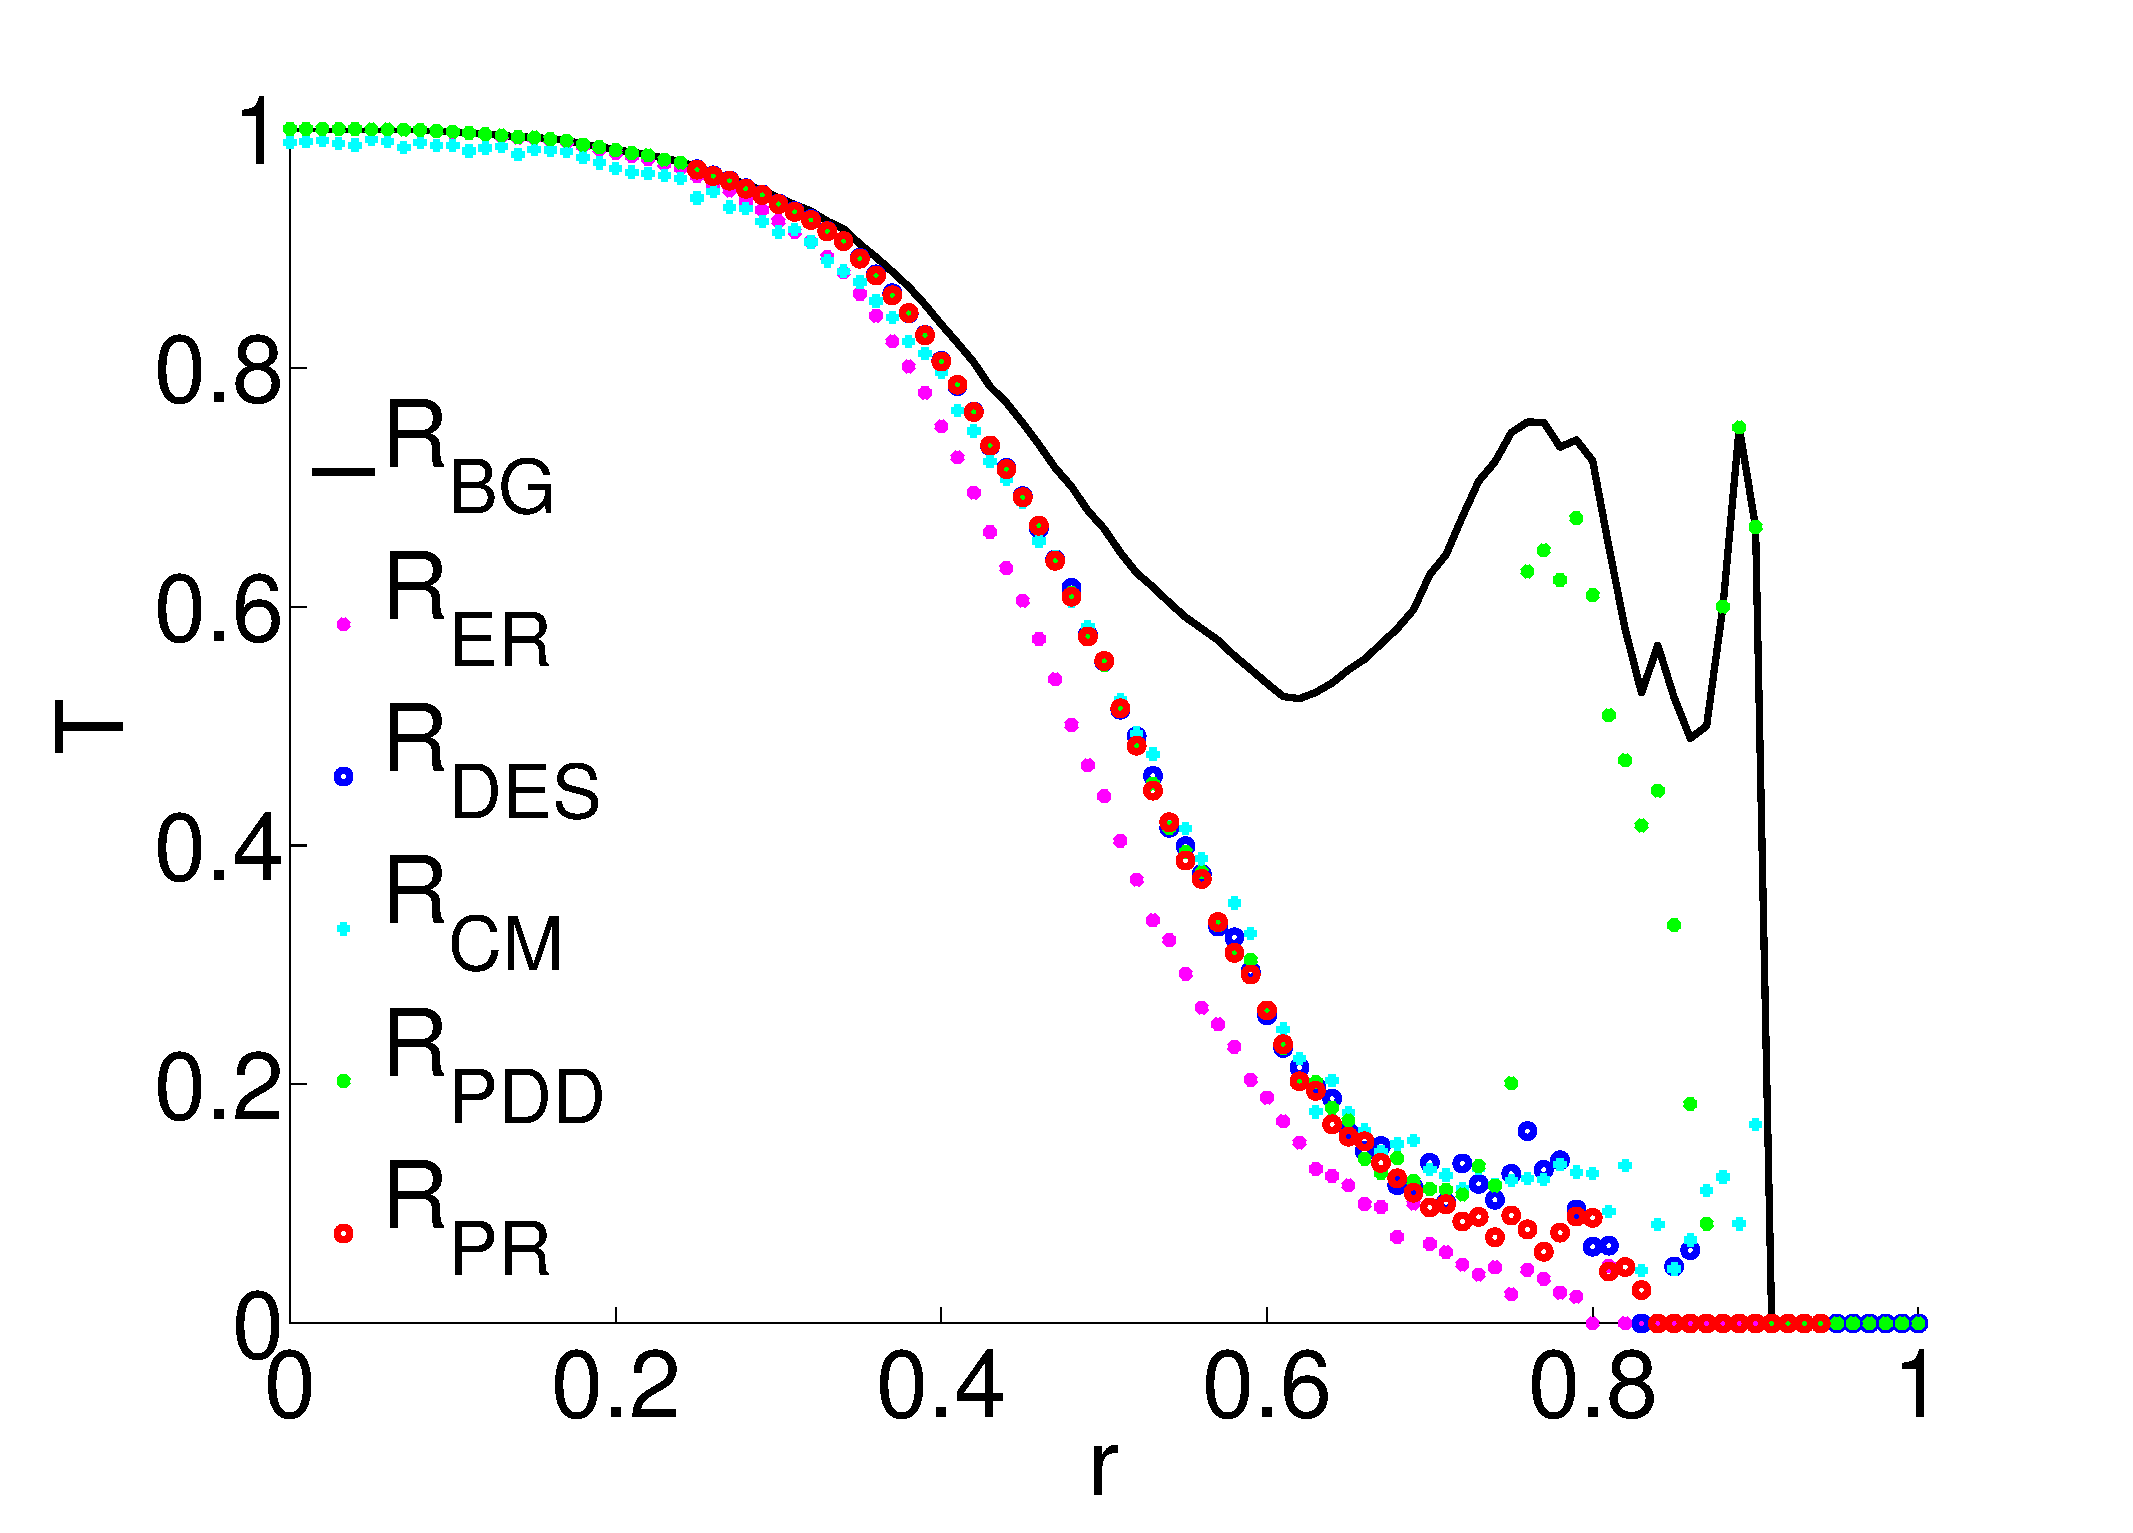
\includegraphics[width=0.48\textwidth, height=55mm]{Figures/Transitivity_Fnc.eps}
	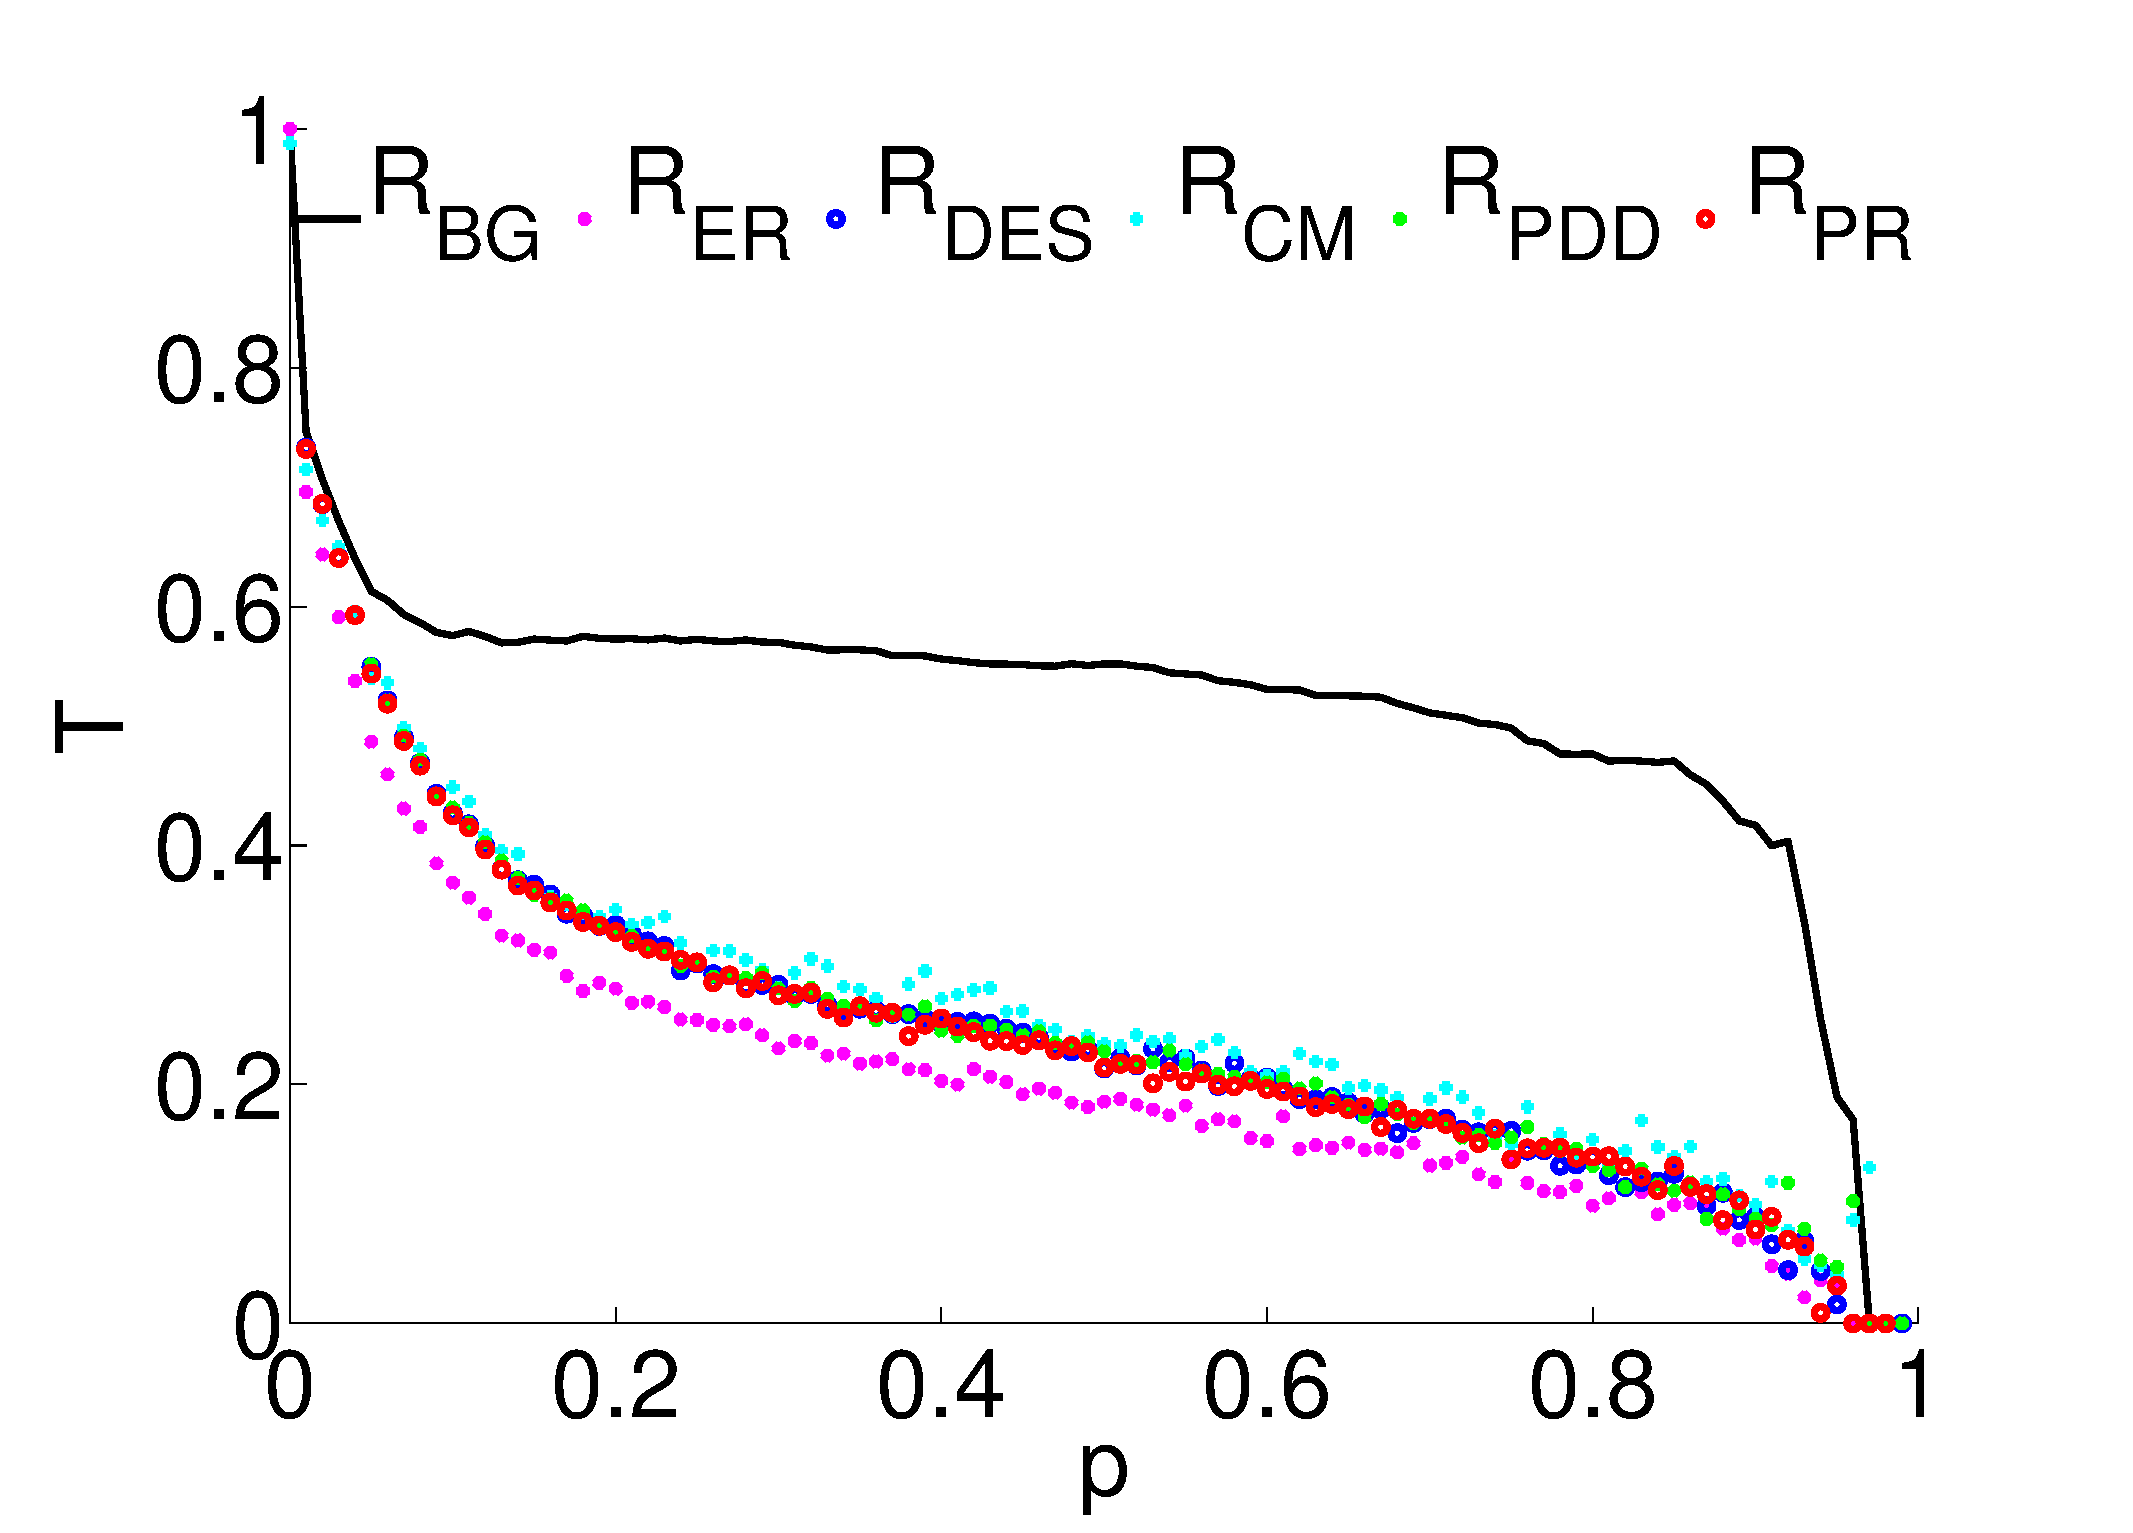
\includegraphics[width=0.48\textwidth, height=55mm]{Figures/Transitivity_Stru.eps} 
    \rule{35em}{0.5pt}
    \caption[Transitivity]{Transitivity of the brain graphs and random graphs of FCM (on the left) and ACM (on the left). }
  \label{fig:Transitivity}
 %\end{tabular}	
\end{figure}


The degree of transitivity is one of the fundamental differences between real world networks and random networks \citep{NEW10}. This difference is more pronounced than the clustering difference between brain graphs and random graphs (see Figures 2.7 and 2.8). $T$ is more effected with $P(k)$ of a network, the more nodes with lower degrees, the higher the $T$ is. ACM related graphs tend to have lower $p(k')$ values distributed among many nodes, whereas FCM related graphs have higher $p(k')$ values distributed among less nodes. This holds even for $R0$ and $Rh$ graphs of FCM in Figure 2.12, that their $P(k)$ is reflected in higher $T$ (see Appendix).



\section{FitzHugh-Nagumo Model for Neuronal Activity Simulation}

An fMRI-BOLD experiment reveals the correlation coefficients between timeseries of BOLD activity among pre-defined brain regions. The empirical functional connectivity matrix (FCM) derived from fMRI-BOLD technique in this project reflects those coefficients among $N=90$ AAL regions at the resting state of the human brain, i.e. no stimulus is introduced to the subject. Despite the lack of any stimulus, the observed fMRI-BOLD signal in the mammalian brain is highly structural and robust at low frequency fluctuations ($<$0.1 Hz) \citep{BIS95, DAM06, VIN07a}. However, the underlying reason of these well organized spatio-temporal dynamics has not yet been completely resolved. The existing models of resting-brain dynamics hypothesize that functional interactions result from a complex interplay between intrinsic brain dynamics and anatomical connections \citep{RUB09}. This section proposes a modeling approach for the ongoing neuronal activity at the brain's resting state, i.e. how  underlying correlated behavior among distant cortical brain regions arises \citep{VUK13}. Once the model is provided with bio-physically plausible parameter ranges with the help of previous studies, the timeseries of nodes in brain graphs will be extracted by means of model simulations and compared to randomly constructed networks. 

The theoretical model of choice for the neuronal activity is the FitzHugh-Nagumo (FHN) system describing physiological states of nerve membrane potential \citep{FIT61, NAG62}. The FHN model will be used to represent the neuronal activity of a nerve cell population, in other words, an AAL node in this project. Local dynamics of a single node will then be globalized in the whole brain network via mutual time delayed interactions among nodes. Here, the time delay $\Delta t_{ij}$ is assumed to arise from a limited signal propagation velocity $v$ between nodes $i$ and $j$. Time delayed interactions are scaled with a coupling strength $c$ \citep{GHO08, GHO08a, DEC09}. Another important parameter for FHN simulations is the threshold $r$ or the probability $p$, values used to extract adjacency matrices from FCM and ACM. The first objective is to investigate plausible $c$, $v$, and $r$ or $p$ ranges at which our simulated neuronal activity of brain graphs is similar to the empirical fMRI-BOLD data. 

The FHN model will also be applied to randomly constructed graphs described in the previous section. The second objective is to identify such regions in the explored parameter space for which the simulated timeseries of the empirically obtained networks are distinguishable from that of randomly constructed graphs. The effects of $c$, $v$, $r$ or $p$ as well as the network characteristics of graphs will be taken into consideration. At the end, it is aimed to gain further insight into the key features of anatomical brain structures by a comparison to randomized networks.  
 
The FHN model is designed to reflect the neuronal activity as a simulated time-series, it does not correspond to the BOLD activity. The last objective of the FHN model is the following: the simulated neuronal activity will be used to infer the BOLD signal via the Baloon-Windkessel hemodynamic model in the last section \citep{FRI00}. 

Subsections 2.5.1 and 2.5.2 will describe a set of non-linear differential equations for the FHN local dynamics, carry out a stability analysis, and introduce a Gaussian white noise effect on the system. The dynamics of a single node will then be globalized via mutual couplings with a second node and the effect of time delay interactions will be demonstrated in Subsection 2.5.3. The last subsection 2.5.4 will embed the complete FHN simulation into a simple graph and the first exemplary time-series of a node will be illustrated. 





\subsection{FHN Model Local Dynamics}

This section aims to demonstrate the local dynamics of a brain node with the FHN model. Here, the node is assumed to be isolated, meaning that it is not connected to any other node in the brain. The FHN model has an activator variable $x$ and an inhibitor variable $y$. Their time evolution is represented with the same implementation as in \citep{GHO08, GHO08a} in the following non-linear differential equations:
\begin{subequations}
\begin{align}\dot{x} = \tau (y + \gamma x - \frac{x^3}{3})  \label{eqn: frobenius 1}\\  \dot{y} = -\frac{1}{\tau} (x - \alpha + b y - I ) \label{eqn: frobenius 2}   \end{align} 
\end{subequations}
where $\tau$ denotes the time constant accelerating $x$ and decelerating $y$, $I$ is the external stimulus parameter and $\gamma$, $\alpha$, $b$ are system parameters. $x$ and $y$ are considered to be counteracting variables capturing alterations of the membrane potential of a neuronal population of around $10^9$ cells. None of the activator or the inhibitor variables include any coupling parameter for the described local activity and additionally $I$ is chosen to be 0 \citep{GHO08}.

The \textit{fixed point} $(x_f, y_f)$ of the system is defined such that there is no change in the variables over time $\dot{y} =\dot{x} = 0 $. The fixed point condition substituted back into equations (2.6a) and (2.6b) yields a set of $nullcline$ equations, 
\begin{subequations}
\begin{align}  y = \frac{x^3}{3} - \gamma x
              \label{eqn: frobenius 3}\\  
               x = \alpha - b y
               \label{eqn: frobenius 4}   \end{align} 
\end{subequations}
where equation (2.7a) will be called $y-nullcline$ and (2.7b) $x-nullcline$ from now on. The stability analysis is performed by calculating eigenvalues of the \textit{Jacobian Matrix}, \textbf{J} at the intersection of nullclines, $(x_f, y_f)$. The  linearization of equations (2.6a) and (2.6b) helps to find  \textbf{J} straightforwardly,
\begin{equation}
%
    \begin{pmatrix}
        \frac{dx}{dt} \\ \frac{dy}{dt}
     \end{pmatrix} = \begin{pmatrix}
        \tau(\gamma - x_f^2) & \tau \\
        -\frac{1}{\tau}     & -\frac{b}{\tau}
     \end{pmatrix}
    \begin{pmatrix}
        x \\
        y
    \end{pmatrix}
%
\end{equation}
where,
\begin{subequations}
\begin{align} \textbf{J} = \begin{pmatrix} \tau(\gamma - x_f^2) & \tau \\ -\frac{1}{\tau}     & -\frac{b}{\tau}   \end{pmatrix}
              \label{eqn: frobenius 5}\\  
 \det \textbf{J} =  b(x_f^2 - \gamma) +1
               \label{eqn: frobenius 6} \\   
\mathrm{tr} \textbf{J} =  \frac{1}{\tau}(\tau^2( \gamma - x_f^2 ) -b)
               \label{eqn: frobenius 7}                 
               \end{align} 
\end{subequations}
. Eigenvalues of \textbf{J} are calculated as the following,
\begin{subequations}
\begin{align} \det \begin{pmatrix} \textbf{J} - \lambda \textbf{I} \end{pmatrix} = 0
              \label{eqn: frobenius 8}\\  
 \lambda^2 - \lambda \mathrm{tr} \textbf{J} + \det \textbf{J} = 0
               \label{eqn: frobenius 9} \\
\lambda_{1,2} = \dfrac{\mathrm{tr} \textbf{J} \pm \sqrt{\mathrm{tr} ^1 \textbf{J}} -4 \det \textbf{J} }{2}               
                \label{eqn: frobenius 10} \\    
\lambda_{1,2} = \dfrac{\tau^2(\gamma - x_f^2)-b \pm \sqrt{(\tau^2(x_f^2-\gamma)-b)^2 - 4 \tau^2 }}{2 \tau}
               \label{eqn: frobenius 11}                 
               \end{align} 
\end{subequations}

The parameters in the FHN model are tuned so that solutions would render a damped oscillatory behavior for each node locally;  $\alpha = 0.85$, $b=0.2$, $\gamma=1.0$ and $\tau=1.25$ \citep{VUK13}. The solution of the condition $\dot{y}=\dot{x}=0$ gives coordinates of $(x_f, \, y_f) = (0.98 \, , -0.67 )$, which is calculated numerically here. All parameters plugged in eigenvalue equation (2.10d) results in $\lambda_1 = -0.056 + 0.996 i$ and $\lambda_2 = -0.056 - 0.996 i$. Since the real parts of both eigenvalues stand below zero, the fixed point is said to be \textit{stable} and since $\lambda_1$ and $\lambda_2$ are complex conjugate pairs, the fixed point can be alternatively called a \textit{stable focus}. Variables $x$ and $y$ are expected to relax onto the fixed point over time.  

\begin{figure}[htbp]
  \centering
	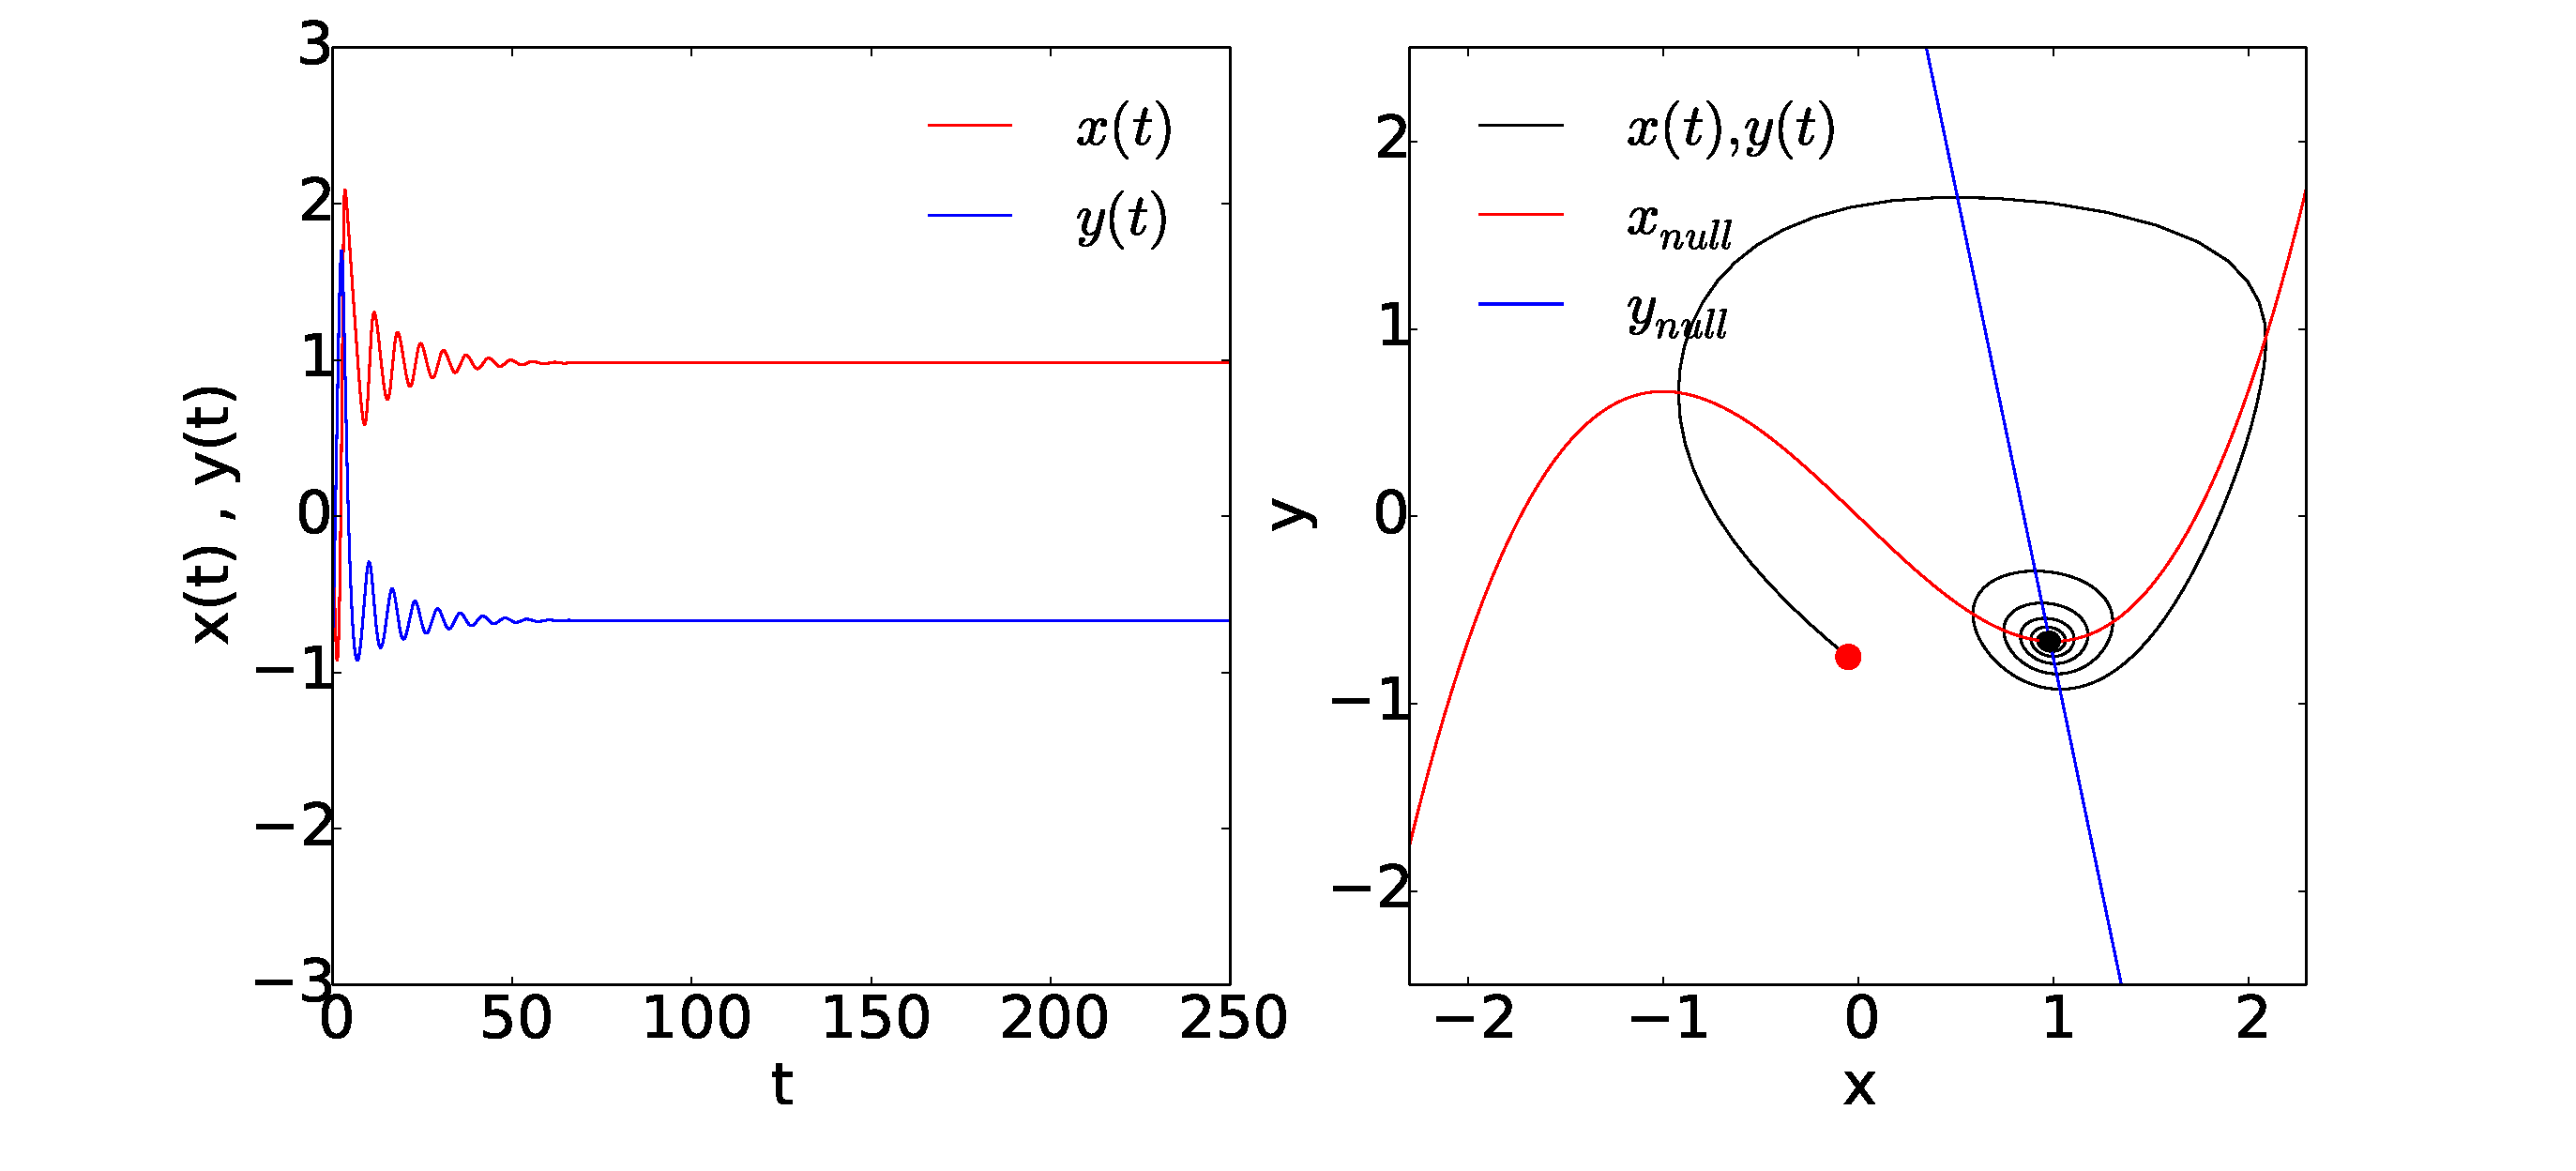
\includegraphics[width=\textwidth]{Figures/FHN_local.eps}
 
    \rule{35em}{0.5pt}
    \caption[FHN Local]{Local dynamics of an isolated node: time evolution of $x$ and  $y$ (on the left) and nullclines on state space together with $x(t),y(t)$ (on the right). The fixed point $(x_f, \, y_f) = (0.98 \, , -0.67 )$ is drawn with a black dot at the intersection of nullclines and initial point $(x_0, y_0)$ is illustrated with a red dot.  }
  \label{fig:FHN Local}	
\end{figure}

The time evolution of $x$ and $y$ resembles damped oscillations at the beginning. Following a rapid excitation and inhibition, both variables converge to the fixed point. The state space illustrates this relaxation over nullclines, a clockwise trajectory starting from a randomly chosen $(x_0, y_0)$ and falling on $(x_f, y_f)$ with smaller and smaller amplitude oscillations. The system is identified in a  quiescent state, or, it is said to be at the onset of instability. The scale of change in $x$  is more pronounced than $y$ due to $\tau$ proportionality in the definition of $\dot{x}$ in the FHN model.  
 
\subsection{Noise Effect}

The local dynamics of a node can be extended by  additional noise terms, 
\begin{subequations}
\begin{align}\dot{x} = \tau (y + \gamma x - \frac{x^3}{3}) + Dn_x  \label{eqn: frobenius 12}\\  \dot{y} = -\frac{1}{\tau} (x - \alpha + b y - I ) + Dn_y \label{eqn: frobenius 13}   \end{align} 
\end{subequations}
where $D$ is the noise strength, and $n_x$ and $n_y$ represent Gaussian white noises. Neither the coordinates of the fixed point nor the eigenvalues are affected by the noise. However, dynamics of the system goes under a change such that the stability will be lost. 

\begin{figure}[htbp]
  \centering
	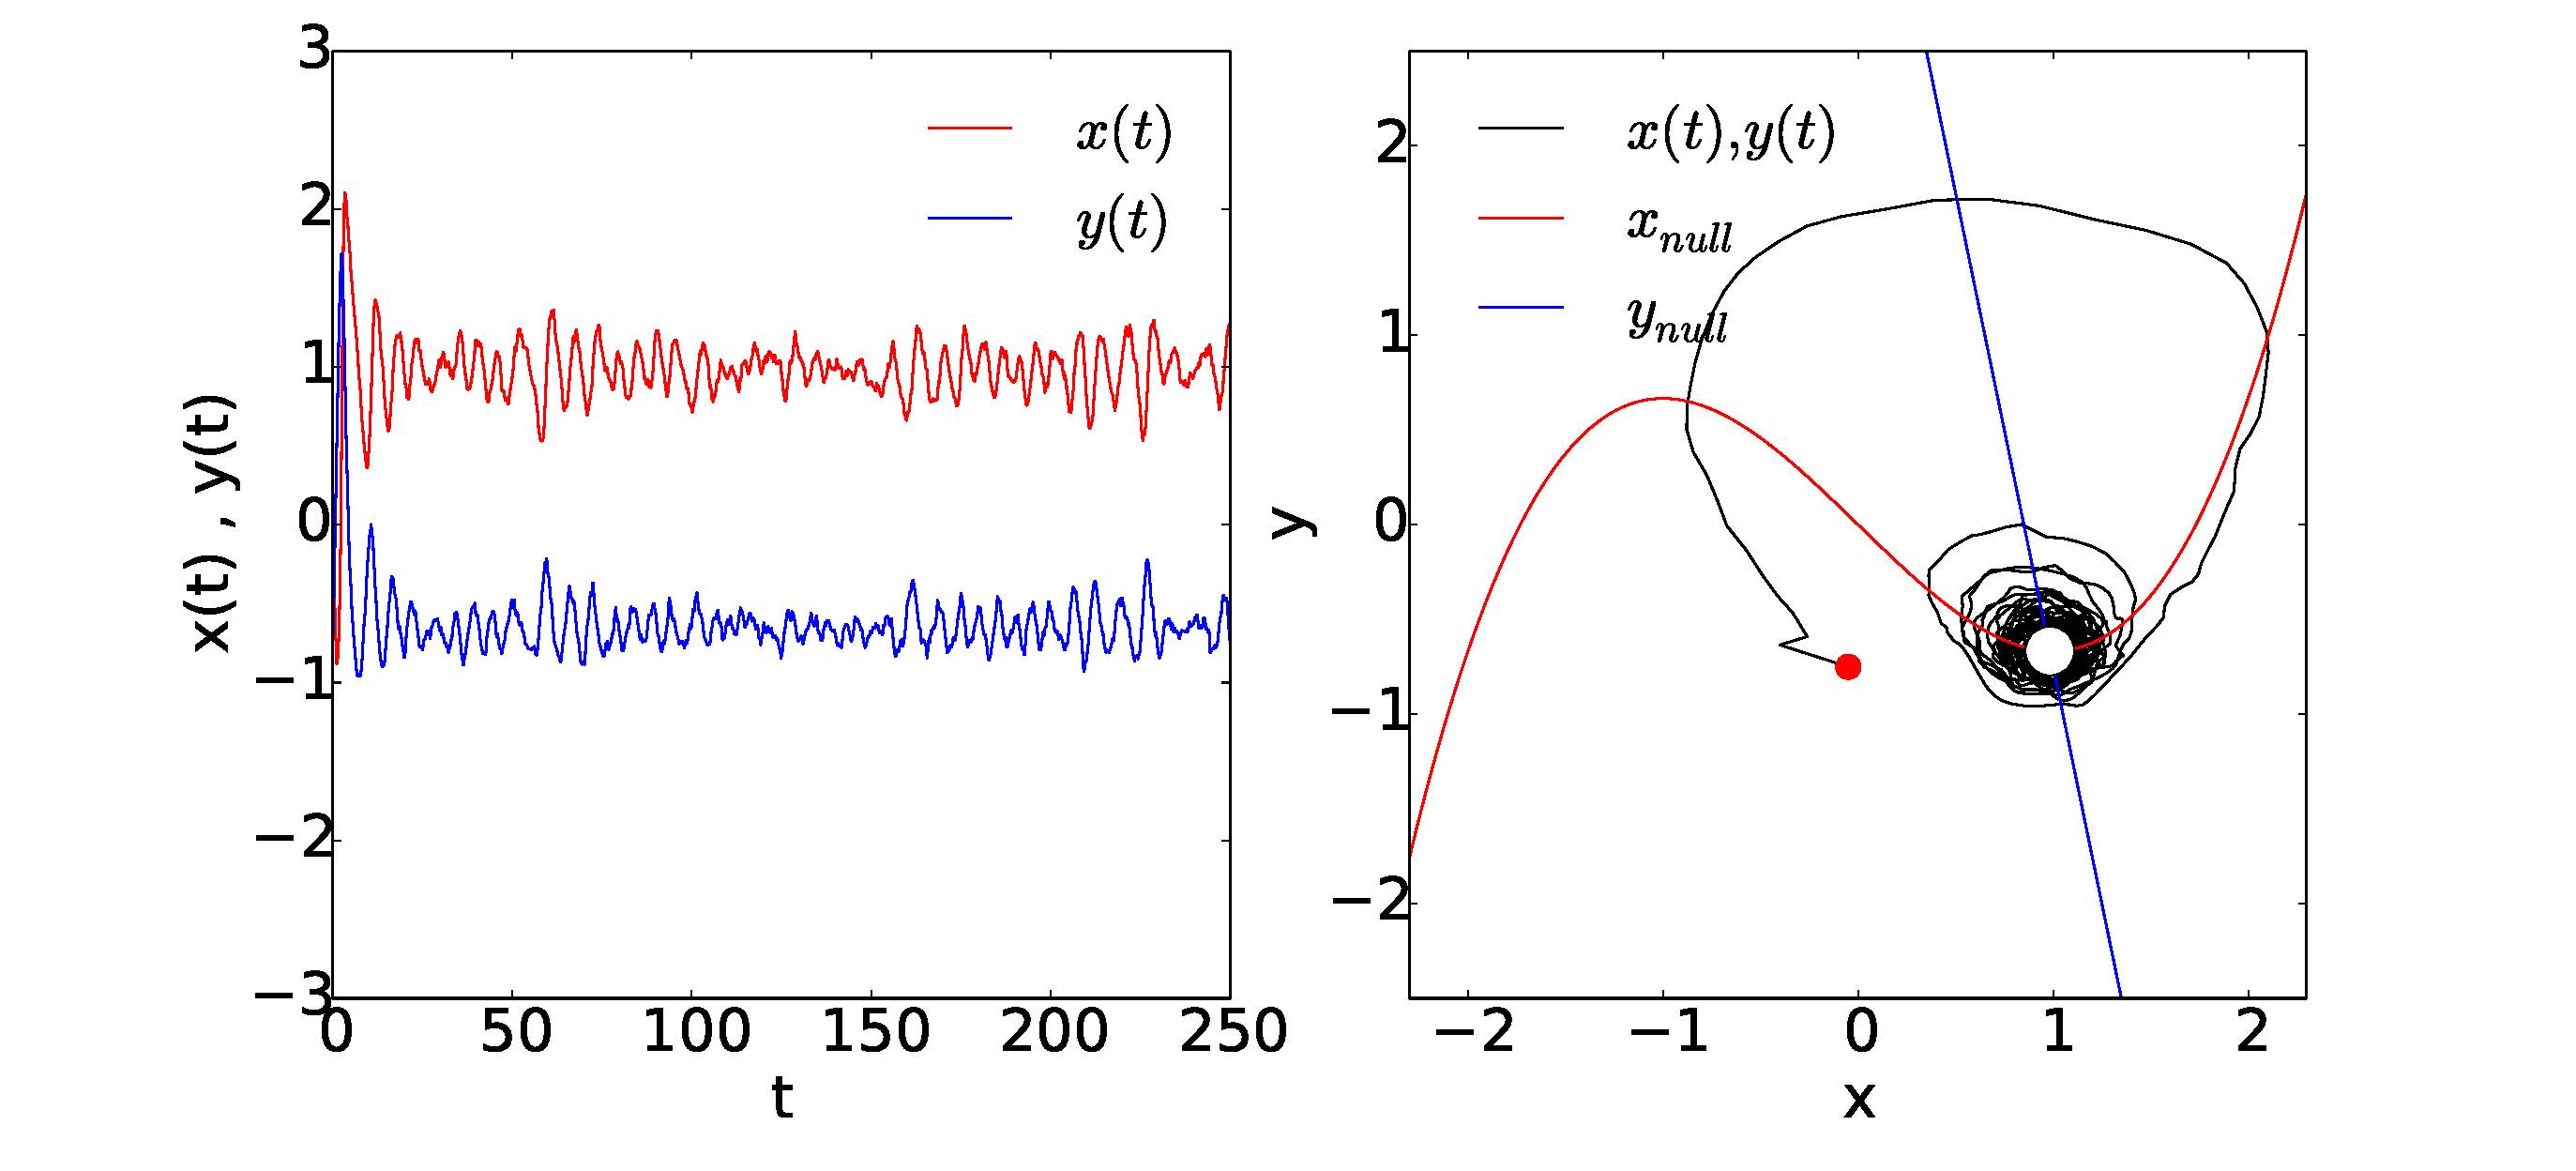
\includegraphics[width=\textwidth]{Figures/FHN_noise.eps}
 
    \rule{35em}{0.5pt}
    \caption[FHN Noise]{Local dynamics of two variables $x$ and  $y$ with same parameters as previously stated, an additional Gaussian white noise with strength $D=0.05$ is added. The fixed point $(x_f, \, y_f) = (0.98 \, , -0.67 )$ is drawn with a black dot in state space where two nullclines intersect.   }
  \label{fig:FHN Noise}	
\end{figure}

The noise drives sub-threshold oscillations as realized in the time evolution of activator and inhibitor. It prevents $x$ and $y$ variables from relaxing on the fixed point, instead, they fluctuate around it. This dynamics marks the onset of instability, and is called "type II excitation" in terms of neuronal dynamics. 


\subsection{Global Dynamics}

This section demonstrates the effect of mutual coupling between two exemplary nodes with FHN model. Now, we consider two nodes connected to each other, either functionally or structurally as in FCM or in ACM. The effect of this connection is captured theoretically with a global coupling term and time delayed interactions, 

\begin{subequations}
 \begin{align}\dot{x_1} = \tau (y_1 + \gamma x_1 - \frac{x^3}{3}) + c [x_2(t-\tau_{12})] +Dn_{x1} \label{eqn: frobenius 14}\\  \dot{y_1} = -\frac{1}{\tau} (x_1 - \alpha + b y_1 - I )+ Dn_{y1} \label{eqn: frobenius 15} \\ \dot{x_2} = \tau (y_2 + \gamma x_2 - \frac{x_2^3}{3}) + c [x_1(t-\tau_{21})] + Dn_{x2} \label{eqn: frobenius 16} \\  \dot{y_2} = -\frac{1}{\tau} (x_2 - \alpha + b y_2 - I ) + Dn_{y2}\end{align} 
\end{subequations}
 
where $c$ is the coupling strength, subindices 1 and 2 stand for corresponding nodes, $\tau_{12}$ and $\tau_{21}$ are time delays required for coupled node interactions and $D$ is the Gaussian white noise strength. For simplicity, the global dynamics are illustrated with same local parameters as before, while time delays are taken to be homogeneous, $\tau_{12}=\tau_{21}=0.5$.

\begin{figure}[htbp]
  \centering
	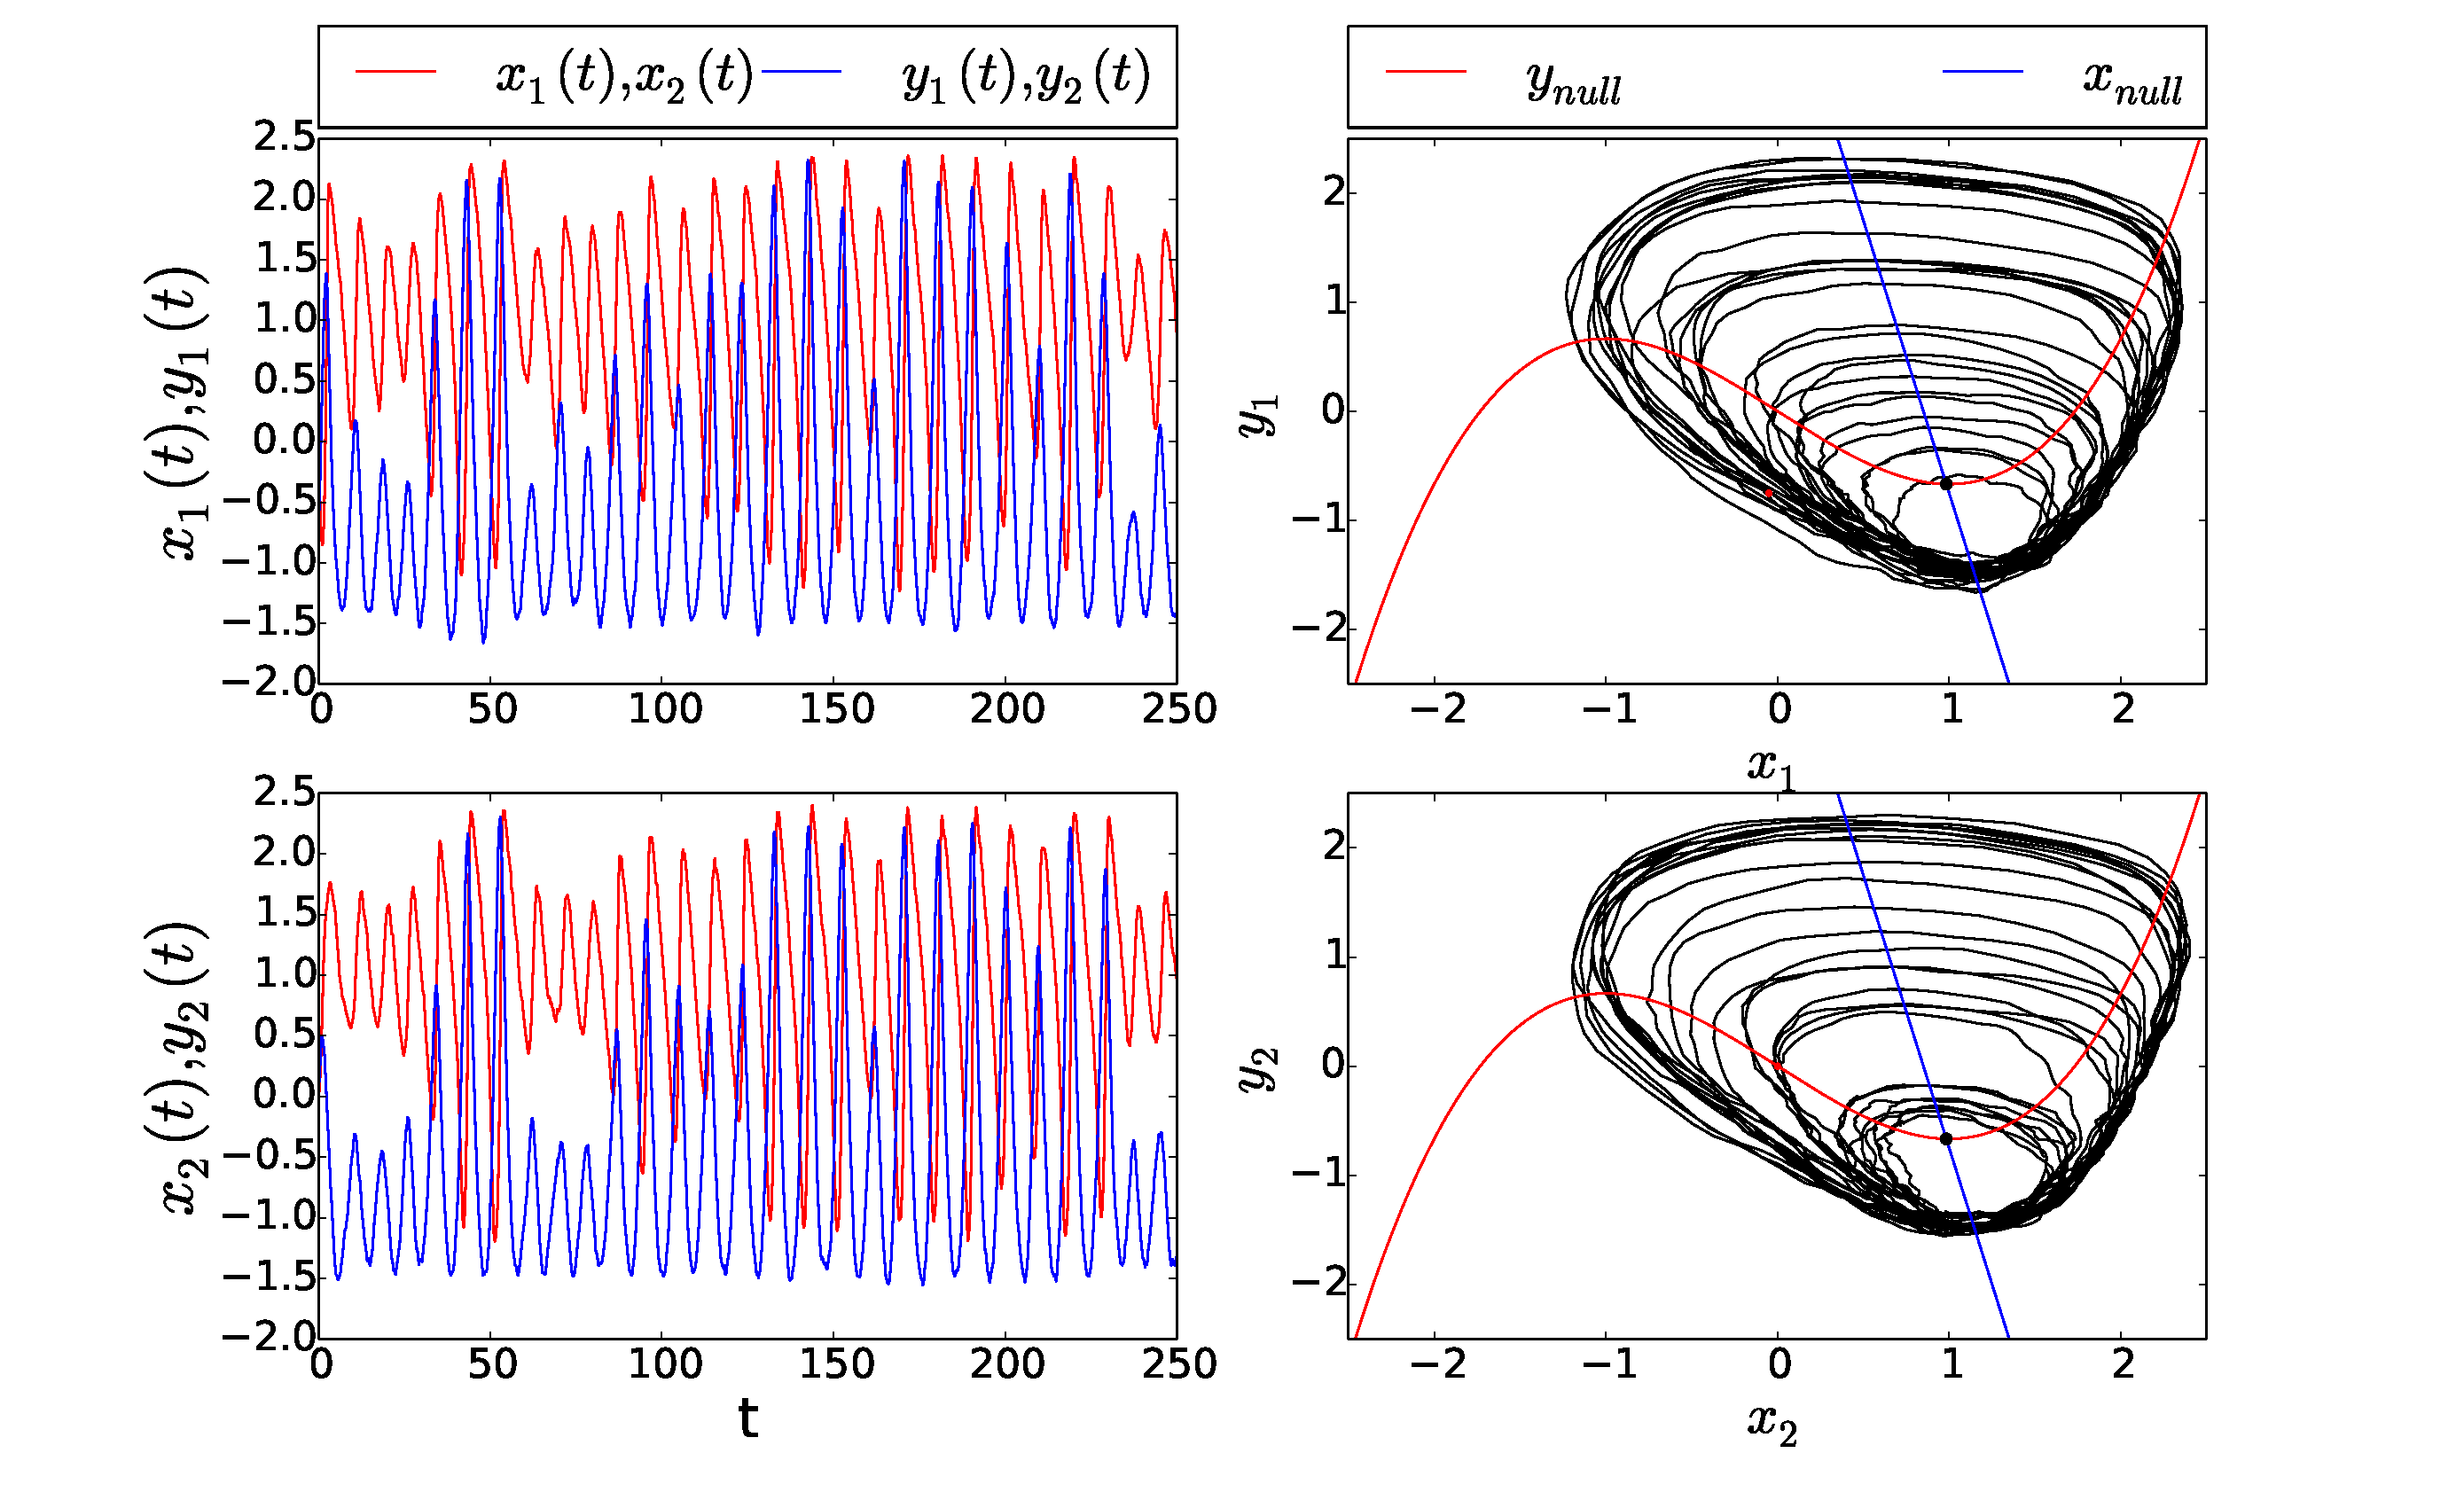
\includegraphics[width=\textwidth]{Figures/FHN_global.eps}
 
    \rule{35em}{0.5pt}
    \caption[FHN Global]{Global dynamics of two nodes with variables $x_1,y_1$ and  $x_2,y_2$. The fixed point is the same for both systems $(x_f, \, y_f) = (0.98 \, , -0.67 )$, it is drawn with a black dot at the intersection of nullclines in state space.}
  \label{fig:FHN Global}	
\end{figure}

The mutual coupling between nodes pushes both systems $(x_1,y_1)$ and $(x_2,y_2)$ to be oscillatory with visibly larger amplitudes in comparison to local dynamics and noise effect in previous figures. The system does not fall on to the fixed point anymore, indicating loss of the stability. 

\subsection{FHN Time Series}

After introducing the local and global dynamical models of nodes, the final version of FHN model to be simulated as the neuronal activity in the complete brain graph or random network is denoted with the following notation \citep{VUK13},  
 
\begin{subequations}
 \begin{align}\dot{x_i} = \tau (y_i + \gamma x_i - \frac{x_i^3}{3}) -c \sum_{j=1}^N a_{ij}x_j(t - \Delta t_{ij}) +Dn_x \label{eqn: frobenius 17}\\  \dot{y_i} = -\frac{1}{\tau} (x_i - \alpha + b y_i - I ) +Dn_y \label{eqn: frobenius 18}   \end{align} 
\end{subequations}

where the index $i$ represents any node among $N=90$ AAL regions, $c$ is coupling strength, $a_{ij}$ is corresponding connectivity unit between nodes $i$ and $j$ in adjacency matrix. This is the crucial link between network analysis part and FHN section. If nodes are connected in a given network, then $a_{ij}=1$, otherwise $a_{ij}=0$. $\Delta t_{ij}$ is the time delay factor arising from finite signal propagation velocity $v$ among nodes. $\Delta t_{ij}$ is calculated as $\Delta t_{ij}=\frac{d_{ij}}{\nu}$ \citep{GHO08, GHO08a, DEC09}, where $d_{ij}$ is the matrix of Euclidean distances between centers of brain regions from which BOLD time series are extracted \citep{KAI06}. The external stimulus is again set to zero $I=0$. The noise ($n_x$, $n_y$) factors are Gaussian white noise distributions, the strength of noise is $D=0.05$, large noise.
 
\begin{figure}[htbp]
  \centering
	\includegraphics[width=\textwidth]{Figures/FHN_graph.eps}
 
    \rule{35em}{0.5pt}
    \caption[FHN Graph]{Two sample graphs to be simulated with FHN model, the upper-most node, say node 1 is not connected at all in first graph (on the left) and connected by 3 edges in second graph (on the right).  }
  \label{fig:FHN Graph}	
\end{figure}


\begin{figure}[htbp]
  \centering
	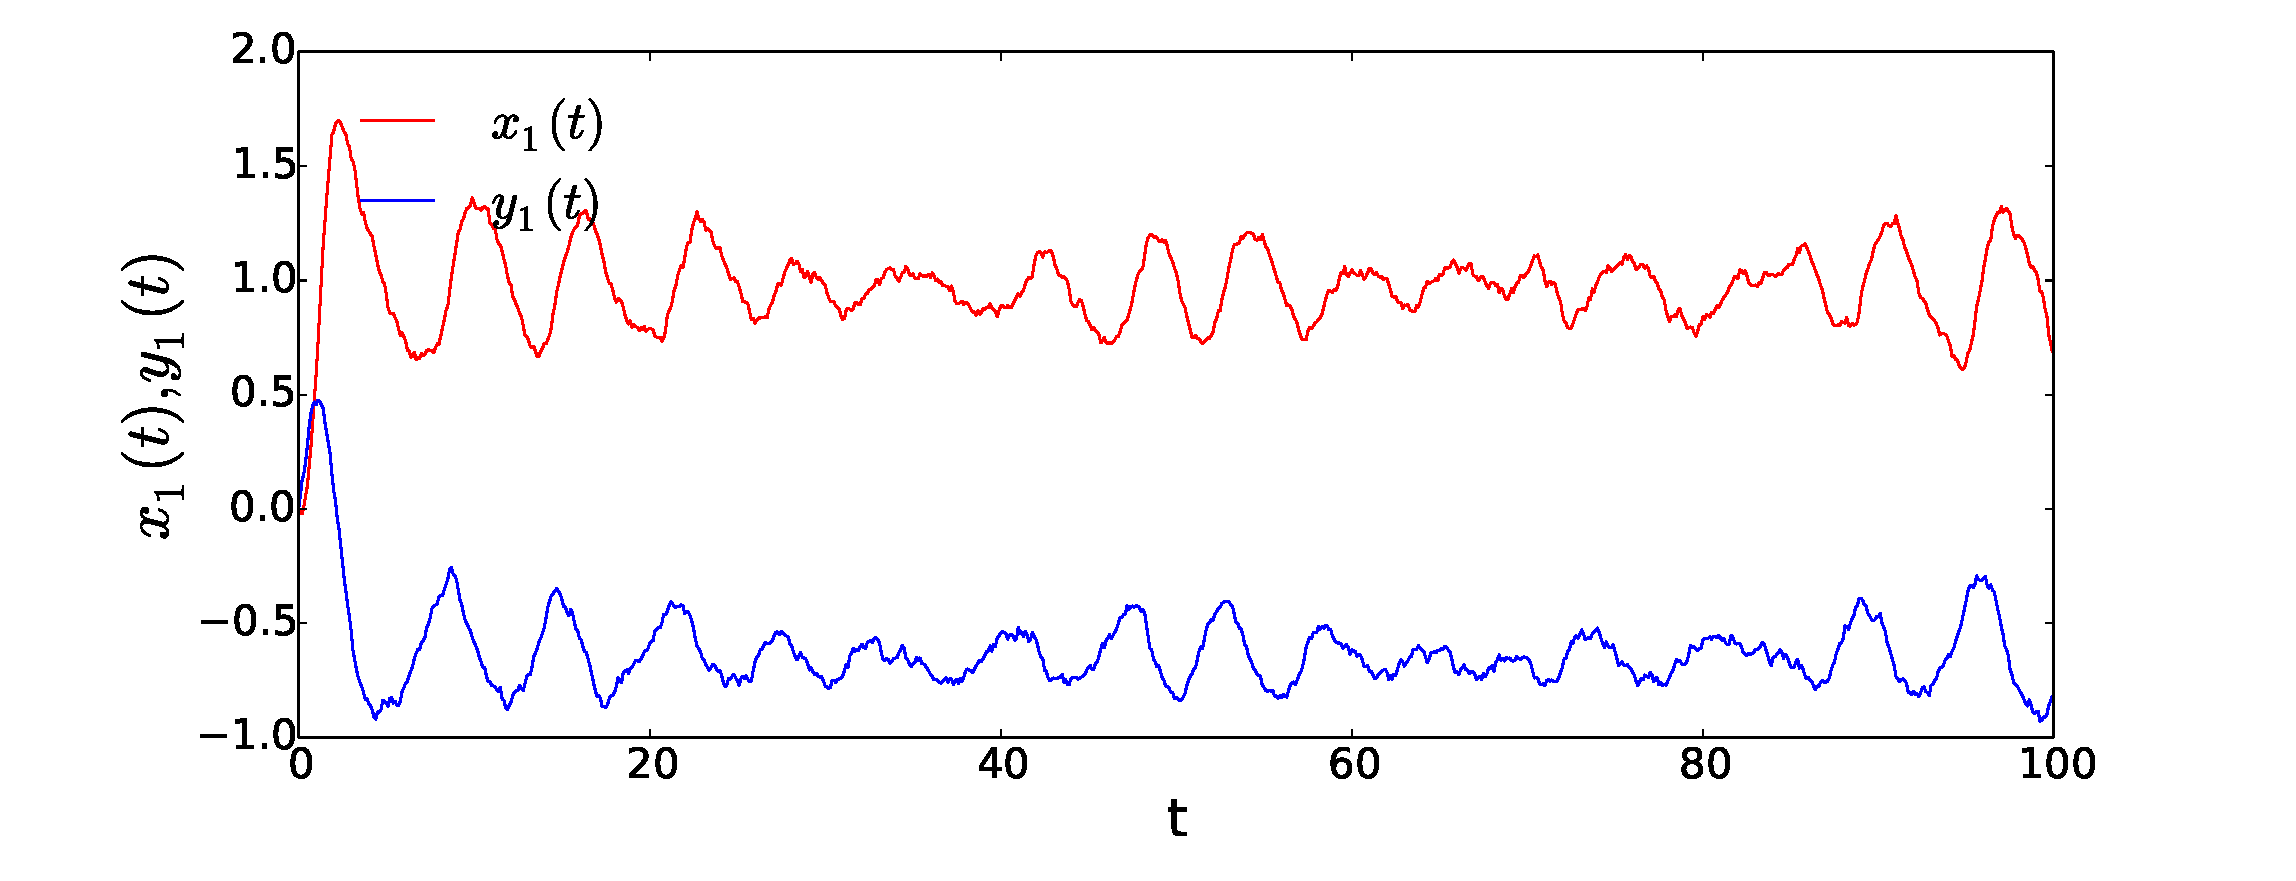
\includegraphics[width=\textwidth]{Figures/FHN_time_1.eps}
 	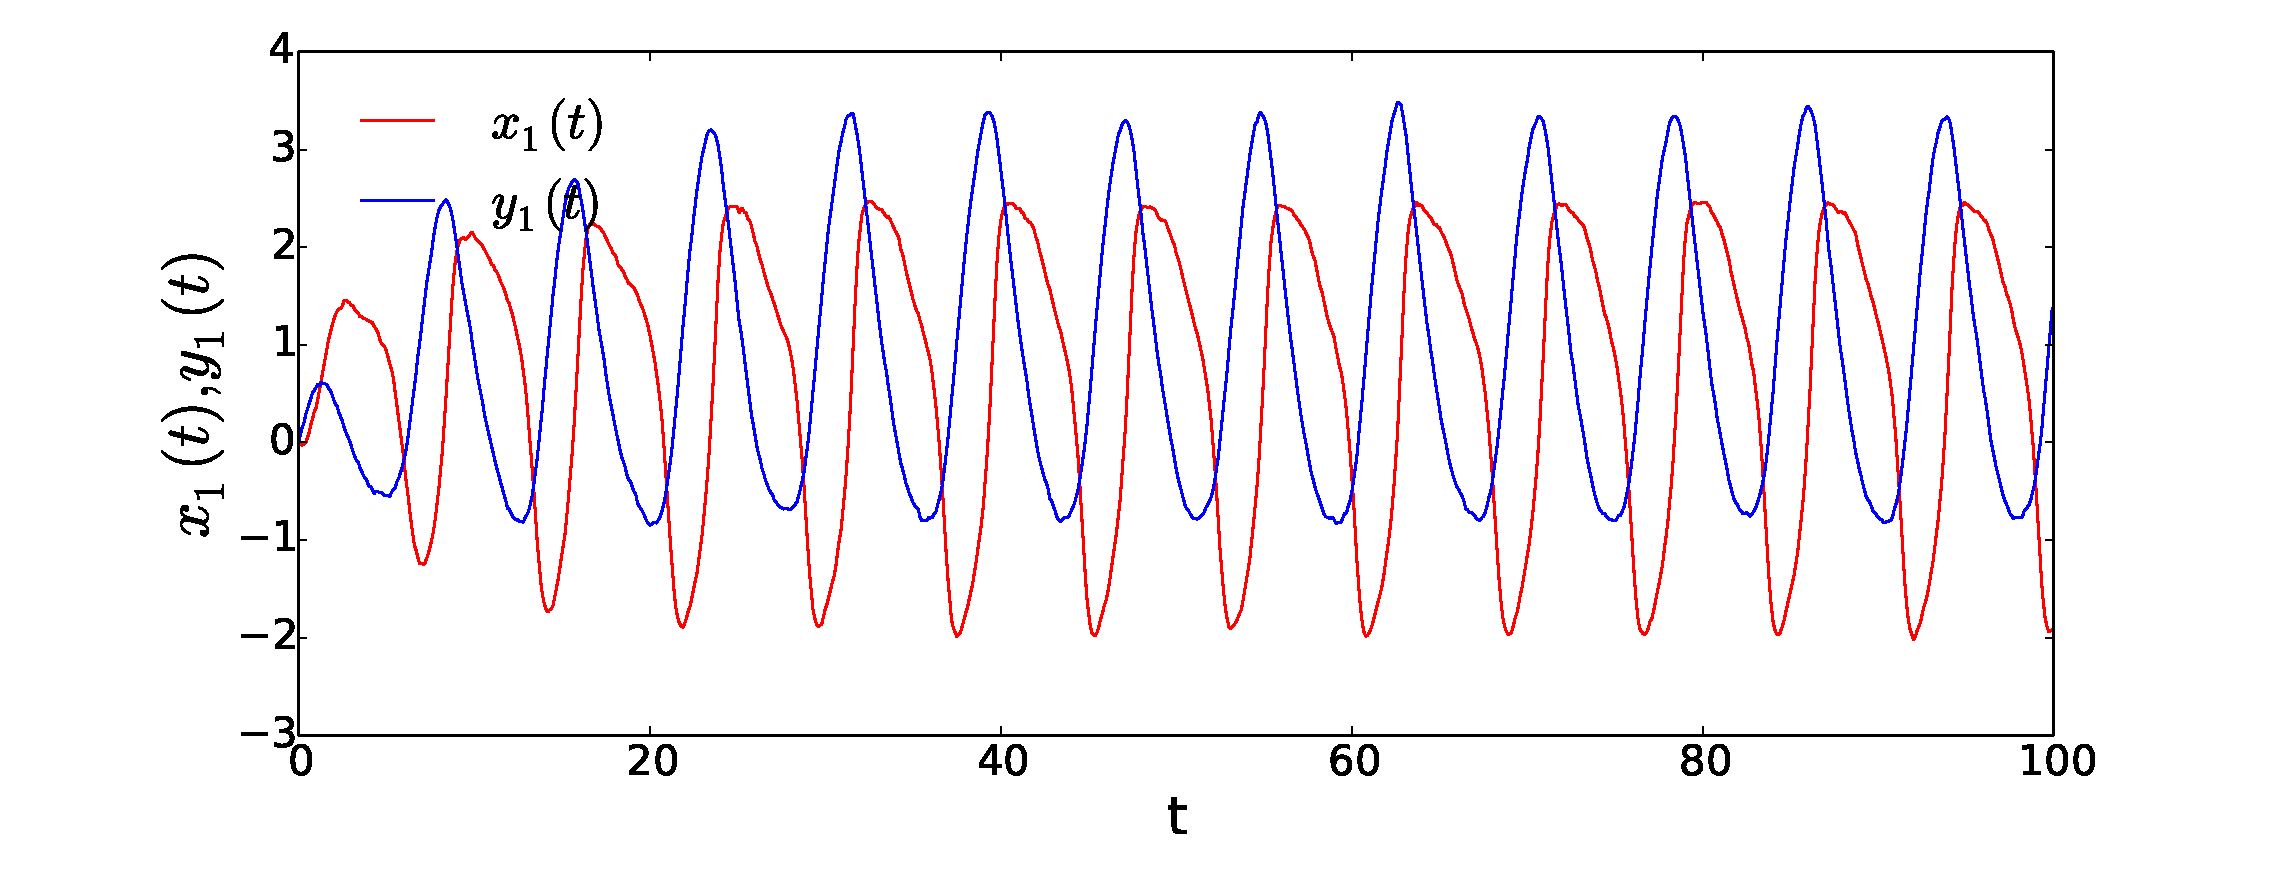
\includegraphics[width=\textwidth]{Figures/FHN_time_2.eps}
    \rule{35em}{0.5pt}
    \caption[FHN Time Series]{Analogous time series of node 1 chosen from graphs illustrated in previous figure. Timeseries at top is of the unconnected node, at down is of 3-edge connected node. All parameters besides $d_{ij}$ matrix are chosen to be biologically plausible. An unrealistic $d_{ij}$ is filled out for corresponding sample graphs in previous figure.  }
  \label{fig:FHN Time Series}	
\end{figure}

The time delay coupled set of ordinary differential equations is solved numerically with \textsc{PYTHON}-module \textsc{PYDELAY}-algorithm based on Bogacki-Sampine method \citep{FLU09a, BOG89}. 


FHN timeseries of node 1, having no edge connections in first graph, is oscillatory, but the scale of oscillations seem to be small. Its dynamical view is in agreement with FHN local dynamics with noise effect. However, when node 1 is connected to 3 other nodes in second graph, then large scaled oscillatory patterns of its activator and inhibitor variables can be observed as a consequence of global coupling terms. 

This section proposed to describe the chosen theoretical model for the neuronal activity. The next step is to study the introduced neuronal dynamics on empirically derived and randomly constructed graphs. $N=90$ nodes  in any given network will be simulated with the complete FHN timseries notation for 7.5 minutes. Then, Pearson correlation coefficients between simulated timeseries of node pairs will be calculated for one graph. A $90X90$ correlation matrix will raise for each FHN simulated network.

FHN model is involved in crucial steps in this Master's project: parameter analysis, distinguishing brain graphs and random graphs and finally extracting BOLD activity. Simulations on brain graphs obtained from FCM and ACM matrices will be compared to the original fMRI-BOLD data in parameter spaces by tuning three parameters in bio-physically plausible ranges: coupling strength $c$ and velocity $v$ as well as a threshold $r$ or probability $p$ value, which is used while constructing adjacency matrices $a_{ij}$ of given graphs. Simulations on random graphs will be used to identify regions in the explored parameter space for which the empirical data differ from that of the random graphs. Not only the effect of tuned parameters $c$, $v$ and $r$ or $p$, but also the contribution of topological measurements of graphs will be taken into account. At the end, FHN timeseries of brain graphs will be simulated further with another theoretical model to capture the BOLD signal, which will be introduced in the next session.   



\section{Balloon-Windkessel Model for BOLD Activity Simulation} 

Blood oxygen level dependent (BOLD) contrast imaging is one of the underlying contrast mechanisms of fMRI to map brain activity at resting state. A BOLD signal is thought to arise from interactions between neuronal activity and regional changes in the surrounding of those active neurons such as blood volume, blood flow and  oxygen level in capillaries. When neuronal activity increases, the blood flow in blood vessels surrounding this neuronal region rises, causing a change in relative amounts of deoxygenated and oxygenated forms of Hemoglobin (dHB and Hb). The difference in magnetic properties of dHb (paramagnetic) and Hb (diamagnetic) is the key ingredient to the observed changes in the magnetic resonance signal. A better understanding of the resting state BOLD signal is required to better interpret neuronal activity. The previous section already proposed  a model for the neuronal activity, the FHN model. This section will introduce a hemodynamic process to capture BOLD activity with a mathematical model known as Balloon model \citep{XYZ98}. 

In addition to the variations in magnetic properties of the blood caused by blood flow in vessels, there are other physiological changes during alteration in neuronal activity that affect the temporal dynamics of BOLD signal, i.e. cerebral blood flow (CBF), cerebral blood volume (CBV) and cerebral metabolic rate of oxygen consumption (CMR$O_2$). Moreover, the BOLD response is subject-dependent: the physiological baseline state of the individual under examination is used to scale its BOLD response, which makes it difficult to interpret the BOLD signal when the baseline state varies \citep{XYZ2013}. Moreover, the sensitivity of a BOLD signal to variations in vascular and metabolic physiology complicates an accurate interpretation. The biophysical descriptions of the BOLD signal are still not fully satisfactory for the resting state. 

Changes in the BOLD signal obtained in an fMRI experiment represent an indirect measure of underlying neuronal activity \citep{VUK14}. The modeled neuronal activity can be used to infer the BOLD signal observed in the fMRI data via the Baloon-Windkessel hemodynamic process, which mediates between a non-linear timeseries and all the measured BOLD response \citep{FRI00}. In short, the Baloon-Windkessel model picks an input signal from neuronal activity timeseries and generates the BOLD activity timeseries as a function of changes in CBF, CBV, CMR$O_2$. The main input of the Baloon-Windkessel model is a neuronal signal in the form of either a spiking rate or a local field potential \citep{SET12}. The neuronal signal in this project will be the normalized FHN timeseries of an activator variable, which describes the excitatory membrane potential dynamics of a neuronal population.       

The study of Friston et al. shows that it is possible to capture ultra-slow frequency oscillations ($<0.1[Hz]$) in the hemodynamic process, given a higher frequency neuronal input for event related responses \citep{FRI00}. Here, the same model will be tested for the resting state activity to find out whether it is possible to extract BOLD activity from FHN-modeled $N=90$ AAL brain nodes. Each brain graph obtained from FCM and ACM data sets will be embedded into the Baloon-Windkessel model, and a parameter analysis will be carried out while comparing resultant BOLD simulations to the fMRI-BOLD empirical data set.

  

\subsection{Hemodynamic Model}

This section is designed to review the Ballon-Windkessel hemodynamic model introduced in Friston et al \citep{FRI00}.  


\begin{figure}[htbp]
  \centering
	\includegraphics[width=\textwidth]{Figures/BOLD_Hemo.eps}
 	\rule{35em}{0.5pt}
    \caption[Hemodynamic Model]{The hemodynamic model for the BOLD activity illustrated in Friston et al. \citep{FRI00}  }
  \label{fig:Hemodynamic Model}	
\end{figure}


\begin{table}[h]
\begin{center}
\caption[BOLD Abbreviations]{Notations and their brief descriptions for hemodynamics in Friston et al. }
\begin{tabular}{ l | c }
  Abbreviation & Description \\
  \hline  \hline                     
  $u(t)$ &      nonlinear input signal  
\\ \hline

  s & blood-flow inducing signal 
\\ \hline
  $\tau_s$ & time constant to describe $\dot{s}$  
\\ \hline  
  $f_{in}$ & CBF (inflow) 
 \\ \hline
 $\tau_f$  & feedback time constant 
\\ \hline  
 $v$    & CBV    
\\ \hline
 $\tau_0$  & mean transit time $\dot{v}$    
\\ \hline 
 $\alpha$  & stiffness exponent
\\ \hline 

  $f_{out}(v, \alpha)$ & CBF (outflow) 
\\ \hline
 $E_0$  & resting net $O_2$ extraction rate 
\\ \hline
 $E(f_{in}, E_0)$    & fraction of $O_2$ extracted from $f_{in}$    
\\ \hline
 $q$    &  dHB content in voxel 
\\ \hline
 $y(t)$    &  output BOLD signal          \\
\hline  
  \hline 
 
%  \hline  
\end{tabular}
\label{table:BOLD Abbreviations}
\end{center}
\end{table}	


The CBF is denoted by two symbols based on its flow direction: $f_{in}$ and $f_{out}$, venous blood inflow and outflow, respectively. The nonlinear neuronal activity $u(t)$ and $f_{in}$ are thought to trigger the blood flow inducing signal $s$. Equation (2.14a) represents time dependent change of this signal $\dot{s}$ depending on $u(t)$, $f_{in}$ and $s$. The three system parameters $\epsilon$, $\tau_s$ and $\tau_f$ are described as following: an efficacy parameter for $u(t)$ to raise up $s$, a time constant for $s$ decay, and another time constant for autoregulatory feedback from CBF, respectively \citep{XYZ1994, XYZ1998}.

Hemodynamics in the brain assumes that alterations in regional CBF are shaped by an underlying neuronal activity. Equation (2.14b) presents the rate of change of $f_{in}$ with a linear transformation on $s$, which can originate from a nonlinear neuronal activity model \citep{XYZ00, XYZFR}. 

The alteration in cerebral blood volume $\dot{v}$ is basically formulated by subtracting $f_{out}$ from $f_{in}$, both rated physiologically with a time constant $\tau_0$, which is also referred to as \textit{mean transit time} \citep{XYZ99}. The Windkessel model contributes to the brain hemodynamics while modeling CBF through CBV:  equation (2.15a) describes a function for $f_{out}$ depending on $v$ and a parameter $\alpha$ (the  \textit{stiffness exponent}) \citep{XYZ99}.    

The change in magnetic properties of blood is expressed with the difference between dHb uptake and release. The dHb uptake is proportional to the blood inflow $f_{in}$ to the venous compartment and available oxygen to be coupled to Hb. The amount of oxygen carried with blood inflow is estimated with a function $E(f_{in}, E_0)$ divided by resting net oxygen extraction rate $E_0$ as given in equation (2.15b) \citep{XYZ98}. The dHb release is proportional to the blood outflow $f_{out}$ and the concentration of dHb in corresponding voxel volume $v$.     

\begin{subequations}
 \begin{align} \dot{s} = \epsilon u(t)- \frac{s}{\tau_s} - \frac{f_{in} -1 }{\tau_f}  \label{eqn: frobenius 19}\\  \dot{f_{in}} = s
\label{eqn: frobenius 20} \\ \dot{v} = \frac{f_{in}}{\tau_0} - \frac{f_{out}(v, \alpha)}{\tau_0} 
\label{eqn: frobenius 21} \\ \dot{q} = \frac{f_{in} E(f_{in}, E_0)}{\tau_0 E_0}- \frac{f_{out}(v, \alpha)}{\tau_0}  \frac{q}{v}  
\
\end{align} 
\end{subequations}

\begin{subequations}
 \begin{align} f_{out}(v, \alpha) = v^{1/ \alpha}
 \label{eqn: frobenius 22}\\  E(f_{in} , E_0) = 1- (1-E_0)^{1/f_{in}} \
\end{align} 
\end{subequations}

Finally, the output BOLD signal is modeled as a function depending on variables $v$, $q$ and parameter $E_0$,  

\begin{equation}
y(t)= \lambda (v,q,E_0) = V_0 (k_1(1-q) + k_2(1- \frac{q}{v}) + k_3(1-v))),
\end{equation} 

where $k_1 = 7E_0$, $k_2 = 2$, $k_3 = 2E_0 - 0.2$, and $V_0$ is the resting blood volume fraction. The set of differential equations for ${\dot{s}, \dot{f_{in}}, \dot{v}, \dot{q}}$ is numerically integrated with Euler's method with step size $dt=10^{-3}$ numerically. The six unknown parameters $\epsilon$, $\alpha$, $\tau_0$, $\tau_f$, $\tau_s$ and $E_0$ are picked up from realistic ranges given in Friston et al  \citep{FRI00}. 





 
%----------------------------------------------------------------------------------------
 
% Chapter 3

\chapter{Results} % Main chapter title

\label{Chapter3} % For referencing the chapter elsewhere, use \ref{Chapter1} 

\lhead{Chapter 3. \emph{Results}} % This is for the header on each page - perhaps a shortened title

%----------------------------------------------------------------------------------------

\section{FHN}



\begin{figure}[htbp]
 
  \centering
    \includegraphics[width=0.49\textwidth]{Figures/PA_FCM_c_02.eps} 
	\includegraphics[width=0.49\textwidth]{Figures/PA_FCM_v_7.eps} 

	
    \rule{35em}{0.5pt}
  \caption[Parameter Analysis, FCM]{FHN simulated FCM brain graphs, parameter analysis, $v=7[m/s]$ on the left and $c=0.2$ on the right }
  \label{fig:Parameter Analysis, FCM}
 	
\end{figure}  



\begin{figure}[htbp]
 
  \centering
	 \includegraphics[width=0.49\textwidth]{Figures/cor_FCM_sim.eps} 
   	 \includegraphics[width=0.49\textwidth]{Figures/cor_FCM_exp.eps} 

    \rule{35em}{0.5pt}
  \caption[Best correlated FHN simulation, FCM]{Best correlated FHN simulation of FCM brain graph with $c=0.2$, $v=7 [m/s]$ and $r=0.60$ (on the left) and empirical FCM obtained from fMRI-BOLD. $\rho_{e,s} = 0.43$} 
    \label{fig:Best correlated FHN simulation, FCM}
 	
\end{figure}  



\begin{figure}[htbp]
 
  \centering
	 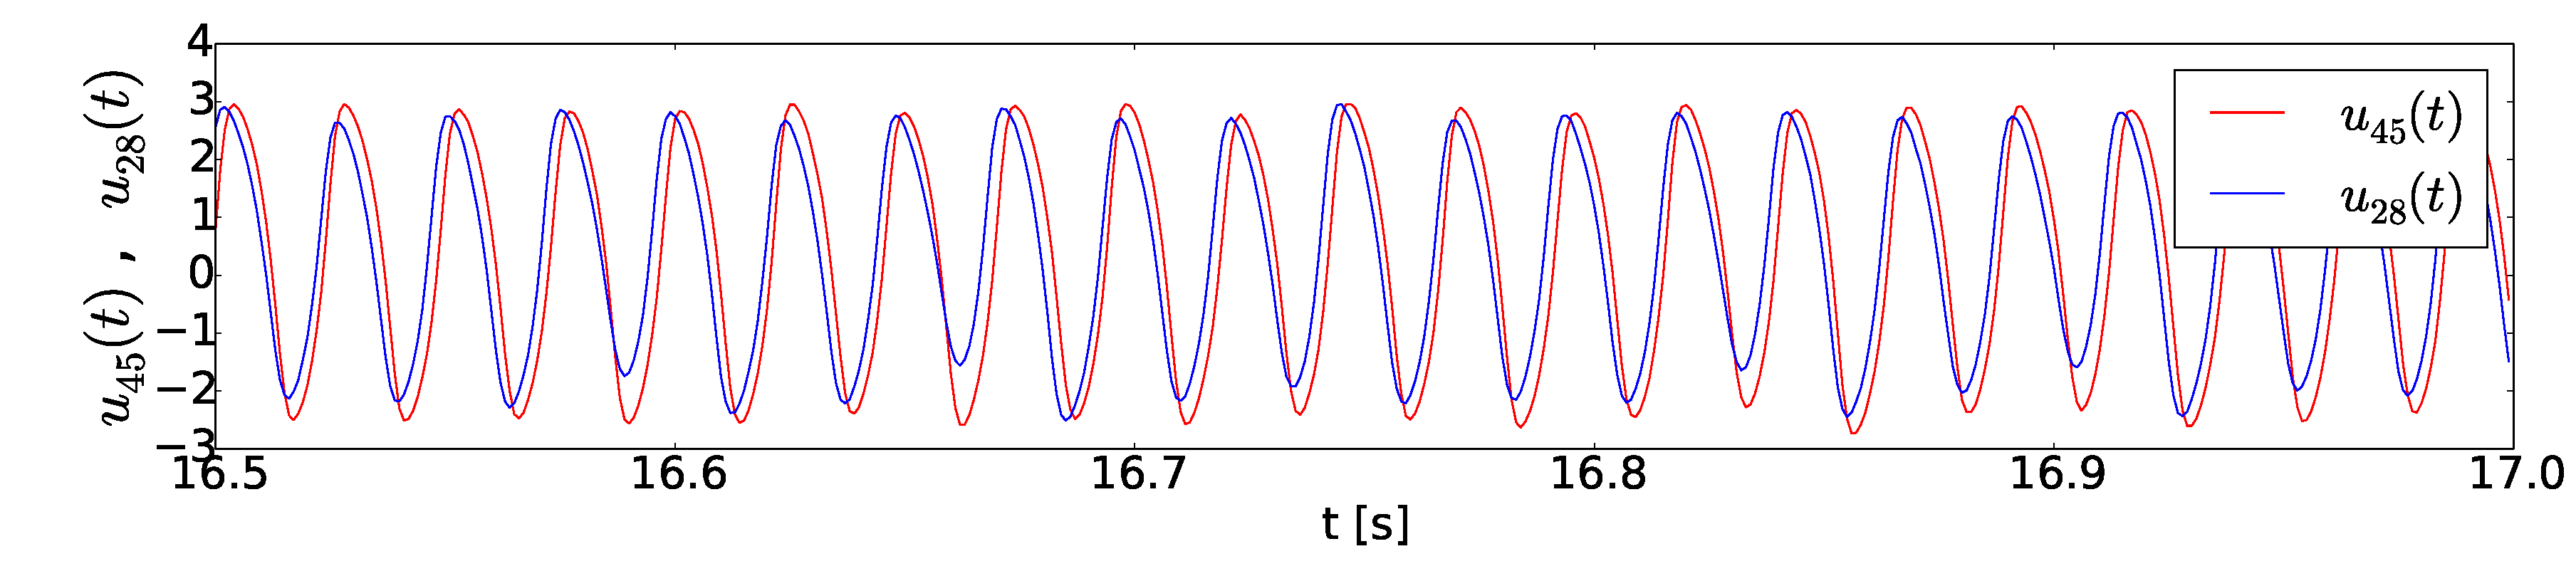
\includegraphics[width=\textwidth]{Figures/cor_FCM_sim_no_best.eps} 
   	 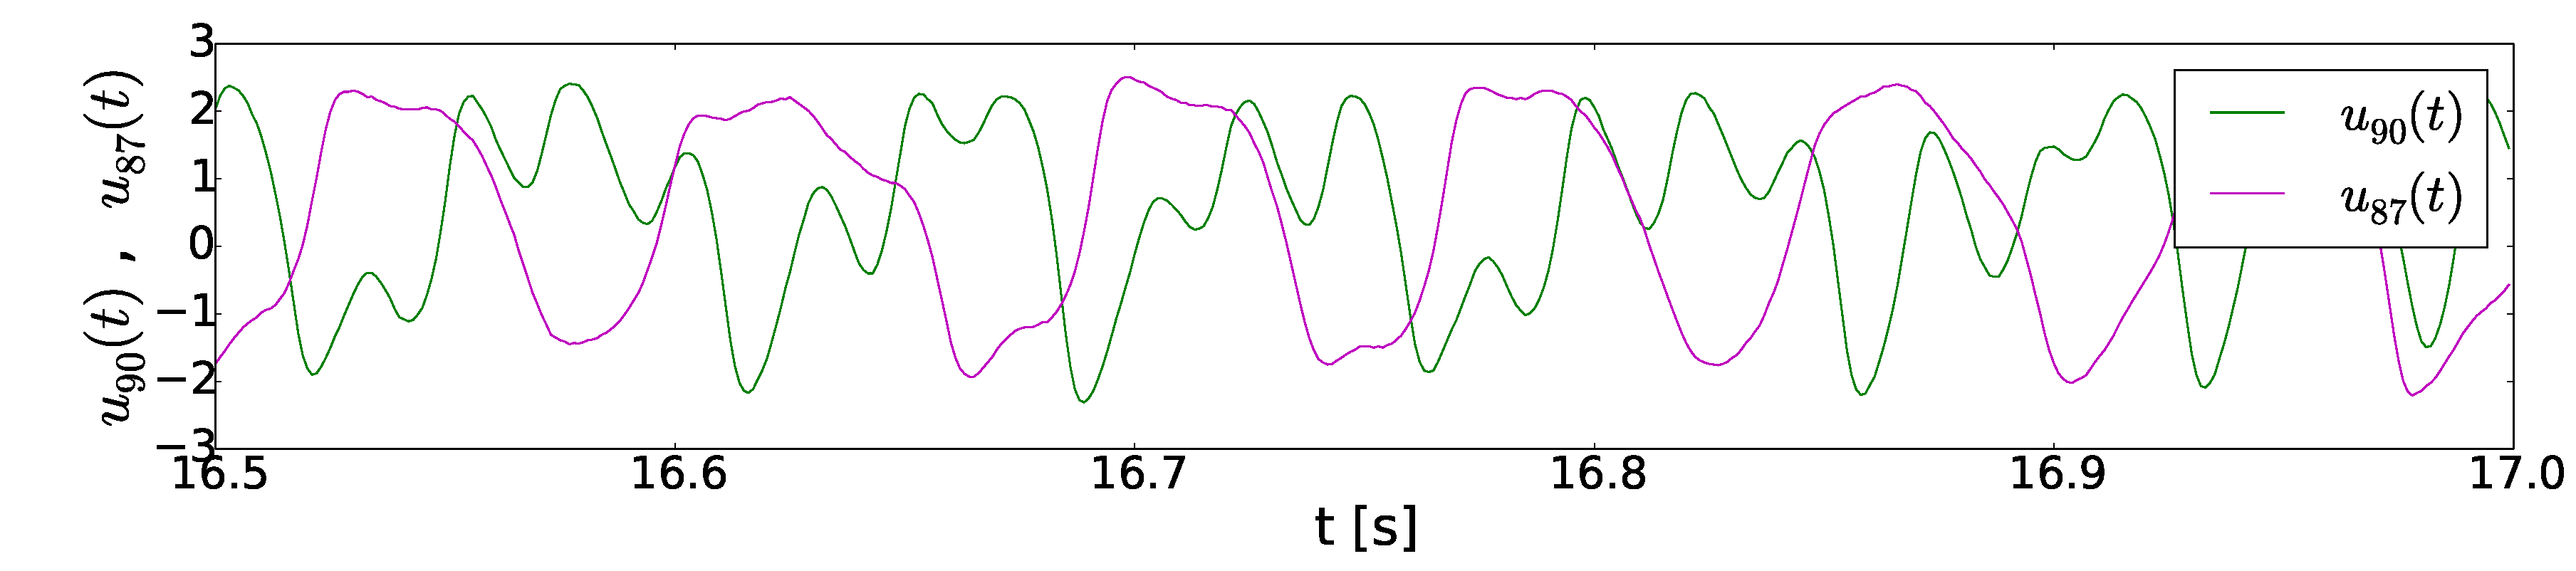
\includegraphics[width=\textwidth]{Figures/cor_FCM_sim_no_worst.eps} 

    \rule{35em}{0.5pt}
  \caption[Neural Activity Node Dynamics, FCM]{Simulated neuronal activity of highly (at top, $\rho_{45,28}=0.88$) and poorly (at bottom, $\rho_{90,87}=0.13$) correlated node couples. Both nodes are chosen from the simulated correlation matrix of FCM in previous figure ($c=0.2$, $v=7 [m/s]$, $r=0.60$).} 
    \label{fig:Neural Activity Node Dynamics, FCM}
 	
\end{figure} 


\begin{figure}[htbp]
 
  \centering
	 \includegraphics[width=0.8\textwidth]{Figures/FFT_FCM.eps} 
   	 %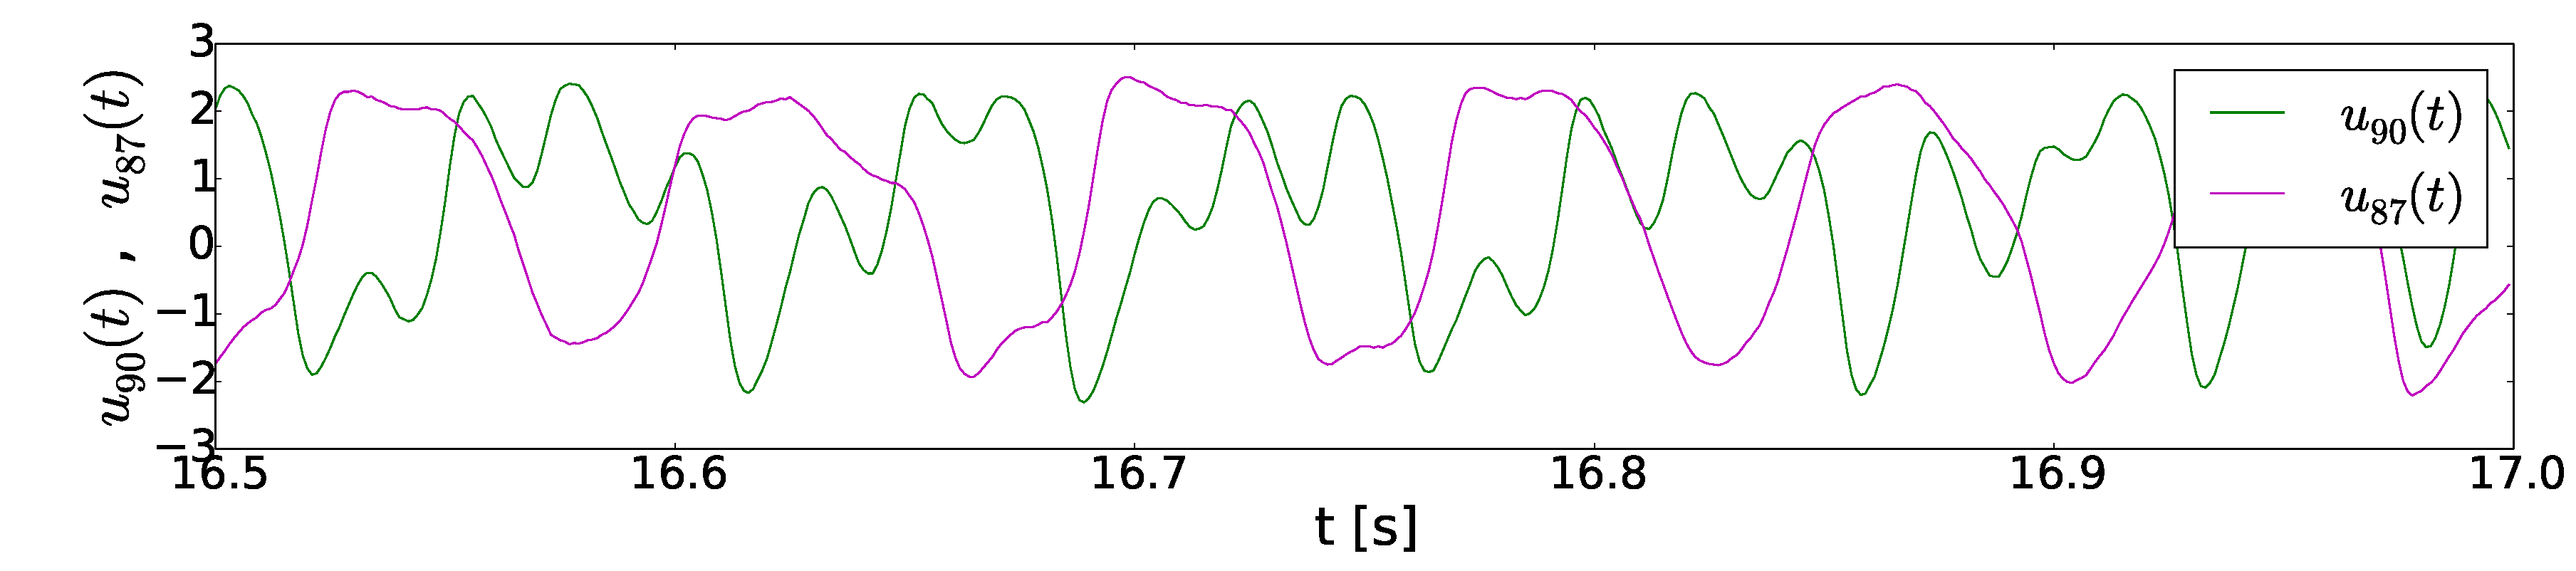
\includegraphics[width=\textwidth]{Figures/cor_FCM_sim_no_worst.eps} 

    \rule{35em}{0.5pt}
  \caption[3D Fourier Transform, FHN, FCM]{3D illustration of fast fourier transform of neuronal activity oscillations corresponding to $N=90$ nodes in FCM simulation with parameters given in Fig.3.2.} 
    \label{fig:3D Fourier Transform, FHN, FCM}
 	
\end{figure}  
 



%\subsection{ACM}

\begin{figure}[htbp]
 
  \centering
    \includegraphics[width=0.49\textwidth]{Figures/PA_ACM_c_03.eps} 
	\includegraphics[width=0.49\textwidth]{Figures/PA_ACM_v_6.eps} 

	
    \rule{35em}{0.5pt}
  \caption[Parameter Analysis, ACM]{FHN simulated ACM brain graphs, parameter analysis, $v=6[m/s]$ on the left and $c=0.3$ on the right }
  \label{fig:Parameter Analysis, ACM}
 	
\end{figure} 





\begin{figure}[htbp]
 
  \centering
	 \includegraphics[width=0.49\textwidth]{Figures/cor_ACM_sim.eps} 
   	 \includegraphics[width=0.49\textwidth]{Figures/cor_ACM_exp.eps} 

    \rule{35em}{0.5pt}
  \caption[Best correlated FHN simulation, ACM]{Best correlated FHN simulation of ACM brain graph with $c=0.3$, $v=6 [m/s]$ and $r=0.50$ (on the left) and empirical ACM obtained from DW-MRI. $\rho_{e,s} = 0.43$} 
    \label{fig:Best correlated FHN simulation, ACM}
 	
\end{figure}



\begin{figure}[htbp]
 
  \centering
	 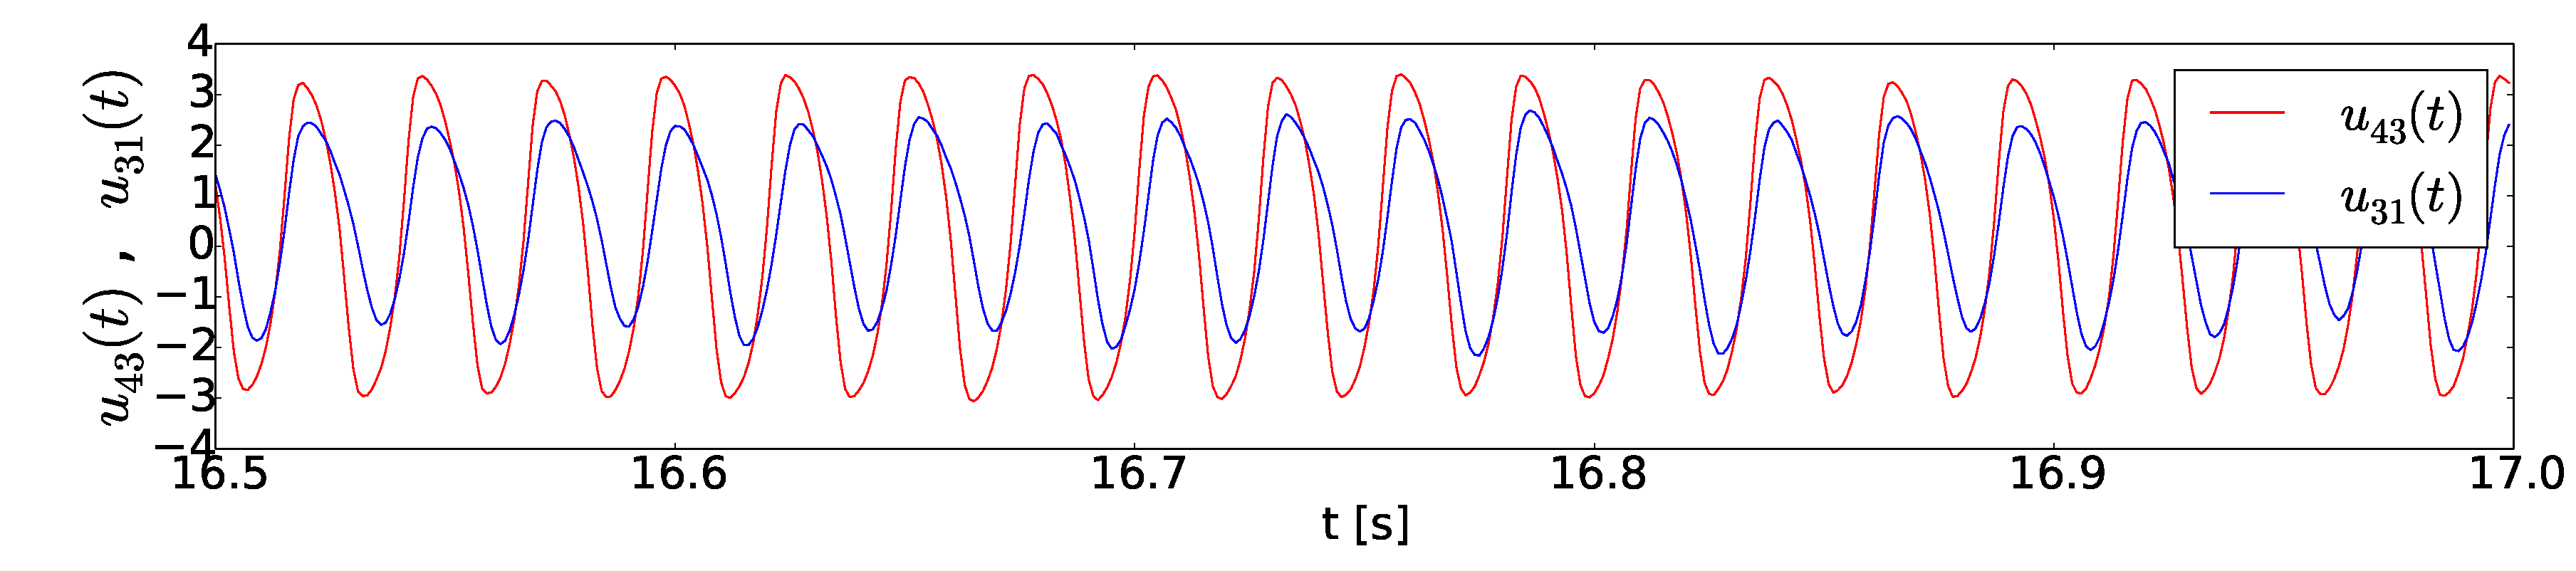
\includegraphics[width=\textwidth]{Figures/cor_ACM_sim_no_best.eps} 
   	 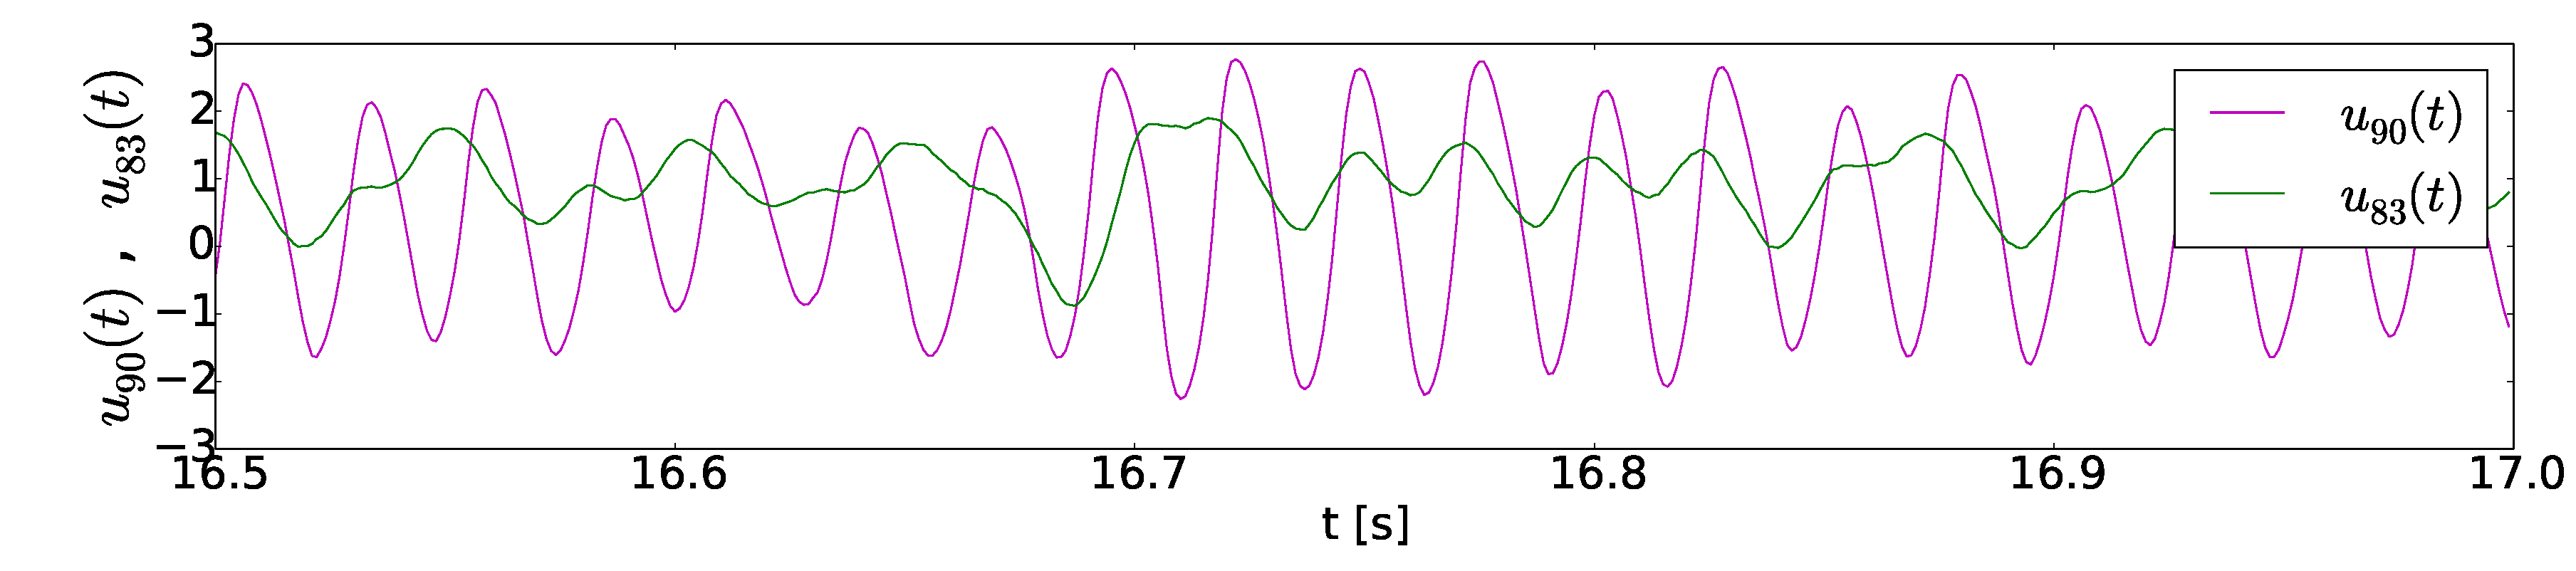
\includegraphics[width=\textwidth]{Figures/cor_ACM_sim_no_worst.eps} 

    \rule{35em}{0.5pt}
  \caption[Neural Activity Node Dynamics, ACM]{Simulated neuronal activity of highly (at top, $\rho_{43,31}=0.86$) and poorly (at bottom, $\rho_{90,83}=0.15$) correlated node couples. Both nodes are chosen from the simulated correlation matrix of ACM in previous figure ($c=0.3$, $v=6 [m/s]$, $r=0.50$).} 
    \label{fig:Neural Activity Node Dynamics, ACM}
 	
\end{figure} 




\begin{figure}[htbp]
 
  \centering
	 \includegraphics[width=0.8\textwidth]{Figures/FFT_ACM.eps} 
   	 %\includegraphics[width=\textwidth]{Figures/cor_FCM_sim_no_worst.eps} 

    \rule{35em}{0.5pt}
  \caption[3D Fourier Transform, FHN, ACM]{3D illustration of fast fourier transform of neuronal activity oscillations corresponding to $N=90$ nodes in ACM simulation with parameters given in Fig.3.6.} 
    \label{fig:3D Fourier Transform, FHN, ACM}
 	
\end{figure}  




\begin{figure}[htbp]
 
  \centering
    \includegraphics[width=0.49\textwidth]{Figures/PA_BOLD_FCM_v_7.eps} 
	\includegraphics[width=0.49\textwidth]{Figures/PA_BOLD_ACM_v_3.eps} 

	
    \rule{35em}{0.5pt}
  \caption[Parameter Analysis, BOLD]{Parameter analysis for BOLD simulations done with FCM (on the left, $v=7 [m/s]$) and ACM (on the right, $v=3 [m/s]$ ). Note that both simulation outcomes are correlated with only empirical FCM. }
  \label{fig:Parameter Analysis, BOLD}
 	
\end{figure} 



\begin{figure}[htbp]
 
  \centering
	 \includegraphics[width=0.49\textwidth]{Figures/cor_BOLD_FCM_sim.eps} 
   	 \includegraphics[width=0.49\textwidth]{Figures/cor_FCM_exp.eps} 

    \rule{35em}{0.5pt}
  \caption[Best correlated BOLD simulation, FCM]{Highly correlated BOLD simulation of FCM brain graph with $c=0.03$, $v=7 [m/s]$ and $r=0.66$ (on the left) and empirical FCM obtained from fMRI-BOLD. $\rho_{e,s} = 0.24$} 
    \label{fig:Best correlated BOLD simulation, FCM}
 	
\end{figure}  





\begin{figure}[htbp]
 
  \centering
	 \includegraphics[width=\textwidth]{Figures/cor_BOLD_FCM_sim_no_best.eps} 
   	 \includegraphics[width=\textwidth]{Figures/cor_BOLD_FCM_sim_no_worst.eps} 

    \rule{35em}{0.5pt}
  \caption[BOLD Activity Node Dynamics, FCM]{Simulated BOLD activity of highly (at top, $\rho_{28,72}=0.75$) and poorly (at bottom, $\rho_{90,81}=0.11$) correlated node couples. Both nodes are chosen from the simulated correlation matrix in previous figure ($c=0.03$, $v=7 [m/s]$, $r=0.66$).} 
    \label{fig:BOLD Activity Node Dynamics, FCM}
 	
\end{figure} 



\begin{figure}[htbp]
 
  \centering
	 \includegraphics[width=0.8\textwidth]{Figures/FFT_BOLD_FCM.eps} 
   	 %\includegraphics[width=\textwidth]{Figures/cor_FCM_sim_no_worst.eps} 

    \rule{35em}{0.5pt}
  \caption[3D Fourier Transform, BOLD, FCM]{3D illustration of fast fourier transform of BOLD activity slow oscillations corresponding to $N=90$ nodes in FCM simulation with parameters given in Fig.3.10.} 
    \label{fig:3D Fourier Transform, BOLD, FCM}
 	
\end{figure}  


\begin{figure}[htbp]
 
  \centering
	 \includegraphics[width=0.49\textwidth]{Figures/cor_BOLD_ACM_sim.eps} 
   	 \includegraphics[width=0.49\textwidth]{Figures/cor_FCM_exp.eps} 

    \rule{35em}{0.5pt}
  \caption[Best correlated BOLD simulation, ACM]{Highly correlated BOLD simulation of ACM brain graph with $c=0.03$, $v=3 [m/s]$ and $r=0.54$ (on the left) and empirical FCM obtained from fMRI-BOLD. $\rho_{e,s} = 0.22$} 
    \label{fig:Best correlated BOLD simulation, ACM}
 	
\end{figure}  




\begin{figure}[htbp]
 
  \centering
	 \includegraphics[width=\textwidth]{Figures/cor_BOLD_ACM_sim_no_best.eps} 
   	 \includegraphics[width=\textwidth]{Figures/cor_BOLD_ACM_sim_no_worst.eps} 

    \rule{35em}{0.5pt}
  \caption[BOLD Activity Node Dynamics, ACM]{Simulated BOLD activity of highly (at top, $\rho_{58,59}=0.48$) and poorly (at bottom, $\rho_{90,89}=0.11$) correlated node couples. Both nodes are chosen from the simulated ACM correlation matrix in previous figure ($c=0.03$, $v=3 [m/s]$, $r=0.54$).} 
    \label{fig:BOLD Activity Node Dynamics, ACM}
 	
\end{figure} 





\begin{figure}[htbp]
 
  \centering
	 \includegraphics[width=0.8\textwidth]{Figures/FFT_BOLD_ACM.eps} 
   	 %\includegraphics[width=\textwidth]{Figures/cor_FCM_sim_no_worst.eps} 

    \rule{35em}{0.5pt}
  \caption[3D Fourier Transform, BOLD, ACM]{3D illustration of fast fourier transform of BOLD activity slow oscillations corresponding to $N=90$ nodes in ACM simulation with parameters given in Fig.3.13.} 
    \label{fig:3D Fourier Transform, BOLD, ACM}
 	
\end{figure}  








% Chapter 4

\chapter{Conclusion and Discussion}  % Main chapter title

\label{Chapter4} % For referencing the chapter elsewhere, use \ref{Chapter1} 

\lhead{Chapter 4. \emph{Conclusion and Discussion}} % This is for the header on each page - perhaps a shortened title

%----------------------------------------------------------------------------------------
The project utilizes modeling approaches combined with empirical results to resolve underlying biophysical mechanisms of human brain at resting state. Empirical brain connectivity maps of resting state are obtained from fMRI-BOLD and DW-MRI techniques, revealing functional and anatomical connections among AAL regions, respectively. The modeling approaches are implemented to discover \textit{i)} neuronal activity time-series, \textit{ii)} ultra-slow BOLD fluctuations, and \textit{iii)} to investigate topological properties of brain graphs. Temporal dynamics of neuronal populations is built on FitzHugh-Nagumo (FHN) oscillations \citep{GHO08, VUK13, DEC09, FIT61}. The BOLD activity is inferred via the Balloon-Windkessel hemodynamic model, which takes the normalized FHN time-series as an input \citep{FRI00, VUK13}. The spatial properties of brain graphs are discussed by comparing network measures of brain graphs to randomly constructed graphs with statistical methods \citep{BUL09, RUB09, NEW10}. The research proposal  is capture temporal fMRI-BOLD dynamics through structural connectivity map of brain, while discussing if the spatial topology properties of brain networks are distinguishable than that of random graphs. 

The fMRI-BOLD functional correlation matrix can be recaptured with FHN modeled neuronal activity dynamics at high axonal signal propagation velocity $v>6$ m/s, at intermediate coupling strength $0.1<c<0.4$ and at threshold $0.54<r<0.60$. These parameter ranges are in agreement with previous studies \citep{VUK13, GHO08a}. It is possible to follow traces of highly correlating AAL regions located symmetrically on right and left hemispheres as presented with sub-diagonals in Figure 3.2, left.  

The DW-MRI anatomical correlation matrix can also be imitated with FHN model applied on ACM based brain graphs at $v>4$ m/s, at $0.1<c<0.5$, and at connection probability range $0.18<p<0.70$. The symmetry of empirical correlation matrix is preserved in simulated correlation matrix as seen in Figure 3.6.

Brain graphs are constructed on adjacency matrices, which are binarized empirical FCMs and ACMs via $r$ and $p$, respectively. Here, $r$- and $p$-values yield us to identify network topology of simulated brain graphs, i.e.  $0.54<r<0.60$ corresponds to a network density $0.50< \kappa_{FCM} <0.18$ for FCM graphs, and $0.18<p<0.70$ that of $0.30< \kappa_{ACM} <0.18$ for ACM graphs. The lower boundaries present the limit of \textsc{PYDELAY} module for the numerical solution of time-delayed differential equations of FHN model. The upper limits are restrained with statistical characterizations of brain graphs. Beyond $\kappa_{FCM} <0.18$ and $\kappa_{ACM}<0.18$, less densely connected brain networks exhibit dramatically changing transitivity $T$, shortest pathway $d_{ij}$, small worldness $S$ and assortativity $A$, and simulations become distinctly different from experiment (See Section 2.4 and Appendix B).

One of the key proposals of this master's thesis is to investigate whether it is possible to catch BOLD fluctuations through structural connections in the human brain at resting state. FHN neuronal activity model is promising, but it is not a complete approach for BOLD dynamics due to high frequency oscillations $20$ Hz $< \nu <60 $ Hz of type-II excitable neuronal populations. The inferred Balloon-Windkessel model provides high correlations between FCM based BOLD simulations and fMRI-BOLD data at $c<0.1$, stating that inferred BOLD activity model is plausible at least for the less strongly functionally coupled neurons. However, the principal step is to capture BOLD fluctuations via ACM brain graphs for the thesis proposal. The correlation between ACM based BOLD simulations and fMRI-BOLD is found to be restricted by a Pearson correlation coefficient of $\rho_{e,s}=0.22$ on parameter space $(p,c)$ (Figure 3.9 and 3.12). The coupling strength range is $c<0.1$ for high correlations. Oppositely to FHN neuronal activity simulations, the BOLD fluctuations become more reasonable at very small $c$ for ACM and FCM graphs. $c$ scales the amplitude of neuronal activity oscillations, so, small scaled FHN  oscillating neurons turn out better BOLD activity simulations. The parameter analysis of simulated activity of BOLD signal for ACM graphs can be designed with finer $c$ values with this deduction in future. 

The intrinsic properties of a brain network have a significant effect on its temporal dynamics. This proposal is evidenced statistically, when the modeled neuronal activities of nodes in the brain graph is compared to that of random graphs. The brain graphs are found to be distinguishable than random graphs at specific parameter ranges, i.e. at low coupling strength, in terms of extracted FHN time-series. 
 

 
 
%\input{Chapters/Chapter5} 
%\input{Chapters/Chapter6} 
%\input{Chapters/Chapter7} 

%----------------------------------------------------------------------------------------
%	THESIS CONTENT - APPENDICES
%----------------------------------------------------------------------------------------

\addtocontents{toc}{\vspace{2em}} % Add a gap in the Contents, for aesthetics

\appendix % Cue to tell LaTeX that the following 'chapters' are Appendices

% Include the appendices of the thesis as separate files from the Appendices folder
% Uncomment the lines as you write the Appendices

% Appendix A

\chapter{Automated Anatomical Labeling } % Main appendix title

\label{AppendixA} % For referencing this appendix elsewhere, use \ref{AppendixA}

\lhead{Appendix A. \emph{Automated Anatomical Labeling}} % This is for the header on each page - perhaps a shortened title

The human brain is segmented into $N=90$ cortical and sub-cortical regions according to the Tzourio-Mazoyer brain atlas with the automated anatomical labeling (AAL) template  \citep{TZO02}, such that regions with index $n=\{1,2,...,45\}$ lie on the right hemisphere, whereas $n=\{46,47,...,90\}$ are on the left. The fMRI-BOLD activity is measured from all voxels in an AAL region. FCM reveals the correlation of measured BOLD signal between pairwise combinations of AAL regions. The anatomical connectivity matrix (ACM) used in this project is obtained from the study of Iturria-Medina et al. \citep{ITU08} and it is based on the same $N=90$ AAL regions as in the FCM. Each value in ACM reveals the probability of any 2 AAL regions being connected via axonal fibers. Table A.1 describes AAL regions.
  






\begin{table}[htbp]\small
\begin{center}
\caption[Automated Anatomical Labeling for the Brain Regions]{Anatomical Description of Brain Nodes }
\begin{tabular}{l | l | c}

  
  Index R/L & Anatomical Description & Label \\
  \hline  \hline                     
  1/46 & Precentral & PRE   \\ 
  2/47 & Frontal Sup & F1 \\
3/48 & Frontal Sup Orb    &      F10 \\
4/49 & Frontal Mid        &       F2\\
5/50 & Frontal Mid Orb    &      F20\\
6/51 & Frontal Inf Oper   &    F30P\\
7/52 & Frontal Inf Tri    &     F3T\\
8/53 & Frontal Inf Orb    &      F30\\
9/54 & Rolandic Oper      &      RO\\
10/55 & Supp Motor Area  &      SMA\\
11/56 & Olfactory          &      OC\\
12/57 & Frontal Sup Medial  &   F1M\\
13/58 & Frontal Mid Orb     &   SMG\\
14/59 & Gyrus Rectus         &    GR\\
15/60 & Insula              &      IN\\
16/61 & Cingulum Ant       &   ACIN\\
17/62 & Cingulum Mid        &  MCIN\\
18/63 & Cingulum Post        & PCIN\\
19/64 & Hippocampus         &    HIP\\
20/65 & ParaHippocampal     &  PHIP\\
21/66 & Amygdala           &  AMYG\\
22/67 & Calcarine          &       V1\\
23/68 & Cuneus             &        Q\\
24/69 & Lingual            &   LING\\
25/70 & Occipital Sup      &       O1\\
26/71 & Occipital Mid      &       O2\\
27/72 & Occipital Inf      &       O3\\
28/73 & Fusiform           &    FUSI\\
29/74 & Postcentral        &   POST\\
30/75 & Parietal Sup       &       P1\\
31/76 & Parietal Inf       &       P2\\
32/77 & Supra Marginal Gyrus  &  SMG\\
33/78 & Angular               &   AG\\
34/79 & Precuneus             &   PQ\\
35/80 & Paracentral Lobule    & PCL\\
36/81 & Caudate               & CAM\\
37/82 & Putamen               & PUT\\
38/83 & Pallidum              &  PAL\\
39/84 & Thalamus              & THA\\
40/85 & Heschi                &  HES\\
41/86 & Temporal Sup          &    T1\\
42/87 & Temporal Pole sup     &  T1P\\
43/88 & Temporal Mid          &    T2\\
44/89 & Temporal Pole Mid     &  T2P\\
45/90 & Temporal Inf          &    T3\\
\hline  
  \hline 
 
%  \hline  
\end{tabular}
\label{table:Automated Anatomical Labeling for the Brain Regions}
\end{center}
\end{table}	



% Appendix A

\chapter{Network Characterizations} % Main appendix title

\label{AppendixB} % For referencing this appendix elsewhere, use \ref{AppendixA}

\lhead{Appendix A. \emph{Appendix Title Here}} % This is for the header on each page - perhaps a shortened title

\section{Average Degree}

Degree $k_i$ is simply the number of edges connected to the node $i$. Average degree of a network $\langle k \rangle$ indicates the ratio of total number of edges, \textit{L}, to total number of nodes, \textit{N} in a graph.
 
\begin{equation}
\langle k \rangle = \frac{2L}{N}
\end{equation} 
 
In order not to count each link twice, the total number of edges is divided by $\frac{N}{2}$ instead of $N$. 
 

%\begin{figure}[htp]
%
%  \centering
%
% 
%
%    % Requires \usepackage{graphicx}
%
%    \includegraphics[width=0.45\textwidth, height=60mm]{Figures\Degree_Average_Fnc.eps} 
%
%    \includegraphics[width=0.45\textwidth, height=60mm]{Figures\Degree_Average_Stru.eps}
%
% 
% \label{figur}\caption{Average degrees of the original network and the randomized networks. Left: $R0$ corresponds to the graph of FCM (source is $A\_aal.txt$), right: $R0$ is that of ACM (source is $acp\_w.txt$). Successful $r$ ranges for randomization methods of FCM :  $r_{Ra}=[0,1]$ , $r_{Rd} = [0.25,1.00]$, $r_{Rg} = [0,1.00]$ , $r_{Rh} = [0,1.00]$ , $r_{Rk} = [0.08,0.94]$. Successful $p$ ranges of ACM : $p_{Ra}=[0,0.99]$, $p_{Rd}=[0.01 , 0.99]$, $p_{Rg}=[0, 0.99]$ , $p_{Rh}=[0.05 , 0.98]$. }
%
%\end{figure}
%%



\begin{figure}[htbp]
 
  \centering
	 \includegraphics[width=0.49\textwidth]{../reports/MSc_01_report/Degree_Average_Fnc.eps}
	 \includegraphics[width=0.49\textwidth]{../reports/MSc_01_report/Degree_Average_Stru.eps}
  \caption[Average Degree]{Average degrees of the brain network and the randomized networks, FCM related graphs on the left, ACM related graphs on the right. Successful $r$ ranges for randomization methods of FCM :  $r_{Ra}=[0,1]$ , $r_{Rd} = [0.25,1.00]$, $r_{Rg} = [0,1.00]$ , $r_{Rh} = [0,1.00]$ , $r_{Rk} = [0.08,0.94]$. Successful $p$ ranges of ACM : $p_{Ra}=[0,0.99]$, $p_{Rd}=[0.01 , 0.99]$, $p_{Rg}=[0, 0.99]$ , $p_{Rh}=[0.05 , 0.98]$.} 
    \label{fig:Average Degree}
 	
\end{figure}  


Degree is one of the statistical tools to measure the centrality of network. The higher the average degree is, the more interaction the nodes in the graph have. 

Increasing threshold and probability values diminishes number of edges inverse sigmoidally. As long as the total node numbers, total edge numbers and networks density are all preserved while constructing the random graphs, the average degree remains the same. 

\section{Shortest Pathway}
Shortest pathway $d_{ij}$ is a measure of integration in the network, opposite to the segregation measures. It corresponds to the shortest path length between two nodes in an unweighted graph,  

\begin{equation}
d_{ij} = \sum\limits_{a_{uv} \epsilon g_{i\leftrightarrow j} } a_{uv}
\end{equation}
where $g_{i\leftrightarrow j}$ is the shortest path between nodes $i$ and $j$, $d_{ij}$ is assumed to be $\infty$ for disconnected pairs \citep{RUB10}.


\begin{figure}[htbp]
 
  \centering
	 \includegraphics[width=0.49\textwidth]{../reports/MSc_01_report/Shortest_Pathway_Fnc.eps}
	 \includegraphics[width=0.49\textwidth]{../reports/MSc_01_report/Shortest_Pathway_Stru.eps}
  \caption[Shortest Pathway]{Shortest pathway of the brain graphs and random graphs, FCM graphs on the left and ACM graphs on the right.} 
    \label{fig:Shortest Pathway}
 	
\end{figure}  


The $R0$ network of FCM seems to be less segregated than the randomized networks while $r$ lies between $[0.65,0.95]$. This is the threshold value at which the $R0$ network of FCM begins to get multiple components. The $R0$ network of ACM tends to be more segregated than its random networks. Whenever all the nodes get sparse (approximately $r>0.95$, $p>95$) in both FCM and ACM networks, the shortest pathway is represented as 0. 




\section{Global Efficiency}
The global efficiency $E$ is measured as the average of the inverse shortest pathway,

\begin{equation}
E = \frac{1}{n}\sum\limits_{i \epsilon N} E_i = \frac{1}{n}\sum\limits_{i \epsilon N} \frac{\sum\limits_{j \epsilon N, j\neq i}d_{ij}^{-1}}{n-1 }
\end{equation}

where $E_i$ is the global efficiency of node, $d_{ij}$ is the shortest pathway between nodes $i$ and $j$ \citep{LAT01}. As seen from the equation, global efficiency becomes larger with smaller shortest pathways between nodes. The global efficiency is a measure of the integration in the network. It reveals the strength of connections in a network. Global efficiency measures the ability of a network to transmit information at the global level \citep{XYZDA}.


\begin{figure}[htbp]
 
  \centering
	 \includegraphics[width=0.49\textwidth]{../reports/MSc_01_report/Global_Efficiency_Average_Fnc.eps}
	 \includegraphics[width=0.49\textwidth]{../reports/MSc_01_report/Global_Efficiency_Average_Stru.eps}
  \caption[Global Efficiency]{Global efficiencies of the original networks and random graphs; FCM on left side, ACM on right side.} 
    \label{fig:Global Efficiency}
 	
\end{figure}

All randomly constructed graphs tend to have in slightly higher $E$ than that of brain graphs. If it is easier to visit a node starting from any other node in the graph, the information transmission capacity is expected to be more robust. When Figure B.2 and B.3 are compared, it can be inferred that higher $d_{ij}$ values reveals lower global efficiency in a network. 



\section{Local Efficiency}
The local efficiency $E_{loc}$ is measured as the average of inverse shortest pathways between nodes in neighborhood of a specific node, 

\begin{equation}
E_{loc} = \frac{1}{n}\sum\limits_{i \epsilon N} E_{loc,i} = \frac{1}{n}\sum\limits_{i \epsilon N} \frac{\sum\limits_{j,h \epsilon N, j\neq i} a_{ij} a_{ih}[d_{jh}(N_i)]^{-1}}{k_i(k_i - 1) }
\end{equation}

where $E_{loc,i}$ is the local efficiency of node $i$, $d_{jh}(N_i)$ is the shortest pathway between nodes $j$ and $h$, which are located in neighborhood of node $i$ \citep{LAT01}. Local efficiency measures the ability of a network to transmit information at the local level \citep{XYZDA}.


\begin{figure}[htbp]
 
  \centering
	 \includegraphics[width=0.49\textwidth]{../reports/MSc_01_report/Local_Efficiency_Average_Fnc.eps}
	 \includegraphics[width=0.49\textwidth]{../reports/MSc_01_report/Local_Efficiency_Average_Stru.eps}
  \caption[Local Efficiency]{Local efficiency of the test networks and random graphs} 
    \label{fig:Local Efficiency}
 	
\end{figure}

Brain graphs based on FCM and ACM tend to have higher $E_{loc}$ than their random graphs. Anatomical connectivity matrix related networks have in general higher $E_{loc}$ compared to the functional connectivity matrix related networks. Local information transmit is more efficient in ACM than in FCM. The graphs with larger $E$ in Figure B.3 exhibit lower $E_{loc}$ in Figure B.4.   


\section{Small Worldness}

A small world network is both highly segregated and integrated, a measure of small worldness $S$ was proposed to capture this effect in a single statistic,

\begin{equation}
S = \frac{C/C_{rand}}{L/L_{rand}}
\end{equation}
 
where $C$ and $C_{rand}$ are clustering coefficients, $L$ and $L_{rand}$ are characteristic path lengths of the original and random network respectively \citep{HUM08}. The random network here is constructed with \textit{Erdos-Renyi} method, which has the same number of nodes and links as the reference graph. 

\begin{equation}
L = \frac{1}{n}\sum\limits_{i \epsilon N} L_i = \frac{1}{n}\sum\limits_{i \epsilon N} \frac{\sum\limits_{j \epsilon N, j \neq i }d_{ij}}{n-1 } 
\end{equation}


\begin{figure}[htbp]
 
  \centering
	 \includegraphics[width=0.49\textwidth]{../reports/MSc_01_report/Small_Worldness_Fnc.eps}
	 \includegraphics[width=0.49\textwidth]{../reports/MSc_01_report/Small_Worldness_Stru.eps}
  \caption[Small Worldness]{Small worldness of the brain graphs and random graphs.} 
    \label{fig:Small Worldness}
 	
\end{figure}


In Figure B.5, brain graphs have higher $S$ than random graphs for both FCM and ACM. In comparison to other network measurements, $S$ measure makes brain graphs the most distinguishable than random graphs. At some unique $r$ and $p$ values, random graphs $Rd$ (for FCM) and $Rk$ (for ACM) tend to have quite large $S$, however, this does not change the general high $S$ pattern of brain graphs. Random networks seem to be equally segregated and integrated in general, but the real networks behave differently. 



\section{Assortativity}

Assortativity measures the correlation coefficient between the degrees of all nodes on two opposite ends of a link \citep{RUB10}. Assortativity coefficient $A$ of a network, 

\begin{equation}
A = \frac{\dfrac{1}{l} \sum\limits_{(i,j) \in L}  k_i k_j -  \Big ( \dfrac{1}{2L} \sum\limits_{(i,j) \in L}k_i + k_j  \Big )^2}{\dfrac{1}{2L}\sum\limits_{(i,j) \in L} ( k_i^2+  k_j^2) -\Big ( \dfrac{1}{2L} \sum\limits_{(i,j) \in L}k_i + k_j  \Big )^2 }
\end{equation}

where $L$ is number of edges in, $k_i$ is degree of node $i$ \citep{NEW02a}.


\begin{figure}[htbp]
 
  \centering
	 \includegraphics[width=0.49\textwidth]{../reports/MSc_01_report/Assortativity_Fnc.eps}
	 \includegraphics[width=0.49\textwidth]{../reports/MSc_01_report/Assortativity_Stru.eps}
  \caption[Assortativity]{Assortativity coefficients of brain graphs and random graphs} 
    \label{fig:Assortativity}
 	
\end{figure}

Negative assortativity presents a network having widely distributed high-degree hubs \citep{RUB10}. On the other hand, assortativity coefficients close to $1$ indicates a graph having fine correlated degree nodes. $A$ values follow a very similar pattern around 0 for all the graphs based on ACM as seen in Figure B.6. The degrees of nodes seem not to be significantly correlated. However, $A$ of FCM related networks are more diverse. The degrees of nodes are highly correlated in FCM brain graph, particularly at large $r$, whereas random graphs exhibit anti-correlations among node degrees.   

\section{Degree Distribution}
Degree distribution of a network reflects the probability ($P(k)$) of a node to have a given number of degree ($k$). Degree distribution reveals the resilience of a graph. 

\begin{equation}
 P(k) = \sum\limits_{k' \geq k} p(k')
\end{equation}

where $p(k')$ is the probability of a node having degree $k'$ \citep{BAR99a}. 


\begin{figure}[htbp]
 
  \centering
	 \includegraphics[width=0.8\textwidth, height=110mm]{../reports/MSc_01_report/Degree_Distribution_Fnc.eps}
  \caption[Degree Distribution, FCM]{Heat maps of $P(k)$ of the FCM network. The limits of colorbar are $[log_{10}(10^0), log_{10}(10^1)]$} 
    \label{fig:Degree Distribution, FCM}
 	
\end{figure}



\begin{figure}[htbp]
 
  \centering
	 \includegraphics[width=0.8\textwidth, height=110mm]{../reports/MSc_01_report/Degree_Distribution_Stru.eps}
  \caption[Degree Distribution, ACM]{Heat maps of $P(k)$ of the ACM network. The limits of colorbar are $[log_{10}(10^0), log_{10}(10^1)]$} 
    \label{fig:Degree Distribution, ACM}
 	
\end{figure}




%% Appendix Template

\chapter{Empirical Distance Matrices} % Main appendix title

\label{AppendixC} % Change X to a consecutive letter; for referencing this appendix elsewhere, use \ref{AppendixX}

\lhead{Appendix C. \emph{Empirical Distance Matrices}} % Change X to a consecutive letter; this is for the header on each page - perhaps a shortened title

Write your Appendix content here.

\addtocontents{toc}{\vspace{2em}} % Add a gap in the Contents, for aesthetics

\backmatter

%----------------------------------------------------------------------------------------
%	BIBLIOGRAPHY
%----------------------------------------------------------------------------------------

\label{Bibliography}

\lhead{\emph{Bibliography}} % Change the page header to say "Bibliography"

\bibliographystyle{unsrtnat} % Use the "unsrtnat" BibTeX style for formatting the Bibliography

\bibliography{Bibliography} % The references (bibliography) information are stored in the file named "Bibliography.bib"

\end{document}  